%Latex template designed from scratch by Mary Sylvia %Agwang following a great Youtube video %by Michelle Krummel:

\documentclass[11pt]{article}
%set margins to as stipulated in masters thesis requirements

%% set the page margins as required by the umn Master's thesis formatting
\usepackage{geometry}
\newgeometry{
    top=1in,
    bottom=1in,
    right=1in,
    left=1.5in,
}


%\usepackage[margin=1in]{geometry}
%packages for typing maths stuff
\usepackage{amsfonts, amsmath, amssymb, latexsym, mathrsfs}
\usepackage{lipsum}
%load some packages to include the appendix
\usepackage[toc,page]{appendix}

%add a copyright package
\usepackage{textcomp}

% package for Maths tools
\usepackage{mathtools}
\newcommand\Set[2]{\{\,#1\mid#2\,\}}
%add two packages to add tables and graphics
\usepackage[pdftex]{graphicx} %load the graphics package
\usepackage{epstopdf} % Convert epstopdf
\graphicspath{{./images}} %add a path to the image 
\graphicspath{{./images/FakeBrain-plots}} %add a path to the image
%\graphicspath{{./images/FakeBrain-plots}}
%add path to images
\usepackage{float}
%add package for multiple figures/subfigures
\usepackage{caption} 
\usepackage{subcaption}

\usepackage[export]{adjustbox} %adjust size of figure

%_%%%%7_9_2017
\usepackage{pgfplots}
\usepackage{tikz}
\usepackage{bm}  %make the symbols bold
\usepackage{epstopdf}
%URLs and links and more
%\usepackage{hyperref}
%\usepackage{lipsum} %adds \qed at the end of proofs

%add a package for the table of contents
\usepackage[nottoc, notlot, notlof]{tocbibind}
%prevent latex from using hyphenated words
\usepackage[none]{hyphenat}
%=====change header if this is in appropriate=====%
%creat customed header and footer as follows
\usepackage{fancyhdr} %creates customed header and footer


% Now type within latex preamable


\pagestyle{fancy}
%next clear the default header and footer
 \fancyhead{}
 \fancyfoot{}
% above two commands remove the default numbering
%next place the title in Capital leters and italics to the Left of the Page

%%%%% remove any writing from top and bottom of margins

% \fancyhead[L]{\slshape{Masters thesis paper}}

%%%%%%% now place student's name to the right

% \fancyhead[R]{\slshape Mary Sylvia Agwang}


\fancyfoot[C]{\thepage} %put back page numbers
%the commented commands below remove the ruled lines
% at the header and foot
\renewcommand{\headrulewidth}{0pt}
\renewcommand{\footrulewidth}{0pt}

%The uncommented string of commands in this section (==) % make the headers appear on each page

%===end of setting the headers======================%

%\parindent 0ex

\parindent 0pt
\parskip 1ex
\renewcommand{\baselinestretch}{2}


%The first two of these commands alter the paragraph formatting so that new paragraphs 
% are not indented but separated from the previous one by a small amount of whitespace; the third sets the line spacing.


%%%%%%%%% comment for commands below %%%%%%%%%%%%%%%%%%%%%%%%%%%%%%%%%
%removes paragraphs from sections
%adjust the paragraphs automatically without indendantation in latex
%====spacing description===========================
% this document is made up of 1in margins
% and 1in spacing between paragraphs

%adding new chapters:
\newcommand{
  \mychapter}[2]{
  \setcounter{chapter}{#1}
  \setcounter{section}{0}
  \chapter*{#2}
  \addcontentsline{toc}{chapter}{#2}
}



%%%%%%%%% Must include this to get neat paragraphs %%%%%%%%%%%%%%%%%%%%%%%%
\renewcommand{\baselinestretch}{1} 



%other ways to adjust paragraphs are commented
%\setlength{\parindent}{4em}
%\setlength{\parskip}{1em}


%\newtheorem ---a command used to define theorems, lemmas, definitions and corollaries.
%\theoremstyle{plain}
\newtheorem{Def}{Definition}
\newtheorem{Thm}{Theorem}
\newtheorem{Lem}{Lemma}
\newtheorem{Cor}{Corollary}
\newtheorem{Rem}{Remark}
\newtheorem{Ex}{Example}
\newtheorem{proof}{Proof}
%add a shortcut to make vectors bold
\newcommand{\vect}[1]{\boldsymbol{#1}}
\newcommand{\Bm}[1]{\textbf{#1}}

%abbreviations
\DeclareMathOperator{\E}{\mathbb{E}} %expectation
\DeclareMathOperator{\R}{\mathbb{R}} %real number
\DeclarePairedDelimiter\abs{\lvert}{\rvert}%
\DeclarePairedDelimiter\norm{\lVert}{\rVert}%

%package for an appendix
\usepackage[toc,page]{appendix}

%start writing the content in here
\begin{document}


%include the titlepage
% Title page

\begingroup
        \let\clearpage\relax
        \let\cleardoublepage\relax
        \let\cleardoublepage\relax

\begin{titlepage}
    \begin{center}
        \vspace*{1cm}
        
        \Huge
        An approach for analyzing spike train data using dimensionality reduction\\
        
      
        \vspace{1.5cm}
        
        
        
        A  Thesis\\
        
    SUBMITTED TO THE FACULTY OF THE\\
    
    UNIVERSITY OF MINNESOTA\\
    
         BY\\
         
         \vspace{1.5cm}
         
         Mary Sylvia Ebai Tambe\\
        
           
            \vspace{1.5cm}
           
          
        IN PARTIAL FULFILLMENT OF THE REQUIERMENTS\\
        
           FOR THE DEGREE OF\\
           
         MASTER OF SCIENCE \\
     
         
  
            \vspace{1.5cm}
        
        
        
        Duane Nykamp (Advisor)\\
        
        
        
        \vspace{0.5cm}
        
        
        May 2018
        
        
        
        
    \end{center}
\end{titlepage}


\thispagestyle{empty}
        \endgroup           
        \vfill


%include the copyright page
% Copyright Page

\thispagestyle{empty}

\vspace*{8cm}

\begin{center}
 
 
 \textcopyright  \  \  Mary Sylvia Agwang  2018    
    
    
\end{center}

\vfill



\newpage









\newpage


%include acknowledgement page
% Acknwoledgements page
\thispagestyle{empty}

\begin{center}
    \Large
    
\section*{Acknowledgements}

\end{center}

\vspace{1cm}

First, I would like to thank my thesis advisor Prof.\ Duane Nykamp for  his guidance, invaluable advise and constructive criticism while  writing this paper and throughout my academic journey. The door to Prof.\ Nykamp's office was always open whenever I ran into a trouble spot or had a question about my research or writing. He  allowed this paper to be my own work, but steered me in the right the direction whenever he thought I needed it.


My very special thanks to  the experts who were involved in the examination and evaluation for this research project: Prof.\ Richard McGehee and Prof.\ Galin Jones.  Without their passionate participation and input,  my plan A master's thesis could not have been successfully completed.


I would  like to acknowledge Madeline Handschy as the second reader of this thesis, and I am gratefully indebted to her for her very valuable comments on this thesis.


Finally, I must express my very profound gratitude to my beloved husband, Dr.  Norbert Tambe Ebai  for providing me with unfailing love and continuous encouragement throughout my years in graduate school, and my precious children Kathleen and Neilton, who are the pride and joy of my life. This accomplishment would not have been possible without them.
Thanks to my family and friends for encouraging me to follow my dreams. Special thanks to my father, John Mark Otim, who encouraged me to pursue farther studies and who has been by my side through thick and thin.
Last but not least, words cannot express my deep gratitude for my Guardians Laveeda and Lynn Battle for their
unwaivering support and for encouraging me to believe in my self.






\vfill




\newpage

%include the copyright page
% Dedication page
\thispagestyle{empty}

\vspace*{8cm}


\begin{center}
    
    
Dedicated to my beloved parents, Ms. Rose Asiimwe and Mr.  John Mark Otim


\end{center}


\vfill


\newpage


%include the abstract
% Abstract page

\thispagestyle{empty}

\begin{center}
    \Large
    
\section*{Abstract}


\end{center}

\vspace{1cm}


Our perception of the world is influenced by the way our brains process information received from millions of neurons.
Our senses are based on information sent to the brain in the form of sequences of stereotyped electrical impulses, or spikes.
We attempt to answer a central question: how do we understand and analyze neural responses when their relationship to external variables such as stimuli, location or behavior  is unclear?


Our main innovation is that we  first ignore these external variables and instead look for structure solely within data representing neural activity such as spike trains. Our preliminary results on synthetic data show how the diffusion maps algorithm applied to data preprocessed in a novel way, captures the  one-dimensional manifold corresponding to a simulated rat's movement around a track. Diffusion maps reveals the structure of a one-dimensional manifold within the neural activity, as would be expected from the fact that the neural activity is strongly correlated with the rat's position.





  \vfill





\newpage



\newpage

%%%  Question: how do i remove the numbering off the abstract page??????


%
%start writing the content in here


%===make a title page=================================%
%Write the department for which the paper is for
% and the purpose of the paper
\begin{titlepage}
\begin{center}
\vspace*{1cm}  %move heading slightly below the center
\Large{\textbf{School of Mathematics}}\\ %department 
\Large{\textbf{Preliminary Oral Exam}} %assessment type
% Next insert the title of your paper here
\vfill %create vertical space to to adjust space between
%create a horizonatal line of length 400
\line(1,0){500}\\[1mm]
%Put the title of your paper in huge bold font
\huge{\textbf{ Analysis of spike train data from the CA1 region of the Rat  hippocampus
using dimensionality reduction}}\\[3mm]
% put another subtitle if neccessary
%\Large{\textbf{-This is a sample subtitle-}}\\{1mm}
%insert another horizonatal line to enclose this
\line(1,0){500}\\
\vfill % adjust spacing automatically
By Mary Sylvia Agwang\\
agwan003@umn.edu\\
\today %print the modest current date after typesetting\\

%=====end of title page===============================%
\end{center}
\end{titlepage}


















% 
%start writing the content in here


%===make a title page=================================%
%Write the department for which the paper is for
% and the purpose of the paper
\begin{titlepage}
\begin{center}
\vspace*{1cm}  %move heading slightly below the center
\Large{\textbf{School of Mathematics}}\\ %department 
\Large{\textbf{Preliminary Oral Exam}} %assessment type
% Next insert the title of your paper here
\vfill %create vertical space to to adjust space between
%create a horizonatal line of length 400
\line(1,0){500}\\[1mm]
%Put the title of your paper in huge bold font
\huge{\textbf{ Analysis of spike train data from the CA1 region of the Rat  hippocampus
using dimensionality reduction}}\\[3mm]
% put another subtitle if neccessary
%\Large{\textbf{-This is a sample subtitle-}}\\{1mm}
%insert another horizonatal line to enclose this
\line(1,0){500}\\
\vfill % adjust spacing automatically
By Mary Sylvia Agwang\\
agwan003@umn.edu\\
\today %print the modest current date after typesetting\\

%=====end of title page===============================%
\end{center}
\end{titlepage}


















%%%%%%%%%% Include acknowledgement in table of contents %%%%%%%%%%%%%%%%%%%%%

%% number the acknowledgements, Dedication and abstract using roman numerals

\pagenumbering{roman}

\addcontentsline{toc}{section}{Acknowledgement}
\setcounter{page}{1}

\addcontentsline{toc}{section}{Dedication}

\addcontentsline{toc}{section}{Abstract}



\tableofcontents

\pagenumbering{arabic}

\thispagestyle{empty}
\clearpage
\setcounter{page}{1}

\newpage

%\mychapter{1}{Introduction}
%%set up basic documents within my document
%\section{Introduction/Background (2-3 days)}
\section{Big picture}

Still working on this.....

%---------This should be more general and give a big picture-------------
%----what do you want to accomplish?
%----what is neural activity in general?
%-----why is a low dim model important?
%-----is idea to understand how the brain is working?
%------How is the brain coding information?
%------how can we decode information based on brain activity?
%----what consequences would there be if we found a low dimensional structure?
%----what is the relevance of having a similarity measure?
%-----e.g want to know whether the brain is thinking about similar things 
%----at different brain states/instances
%----why?  --- what does this have to do with the structure of the space



\section{Biological background}
\subsection{Structure of a neuron}
A neuron is a specialized cell in the nervous system that receives, represents and transmits information through a series of electrical pulses called action potentials or spikes. The action potentials are propagated at uniform strength and speed but with varying frequencies. The neuron is the fundamental unit of brain function. The neuron (see  figure \ref{fig:Neuron}) is made of three major parts, namely the dendrites (receive information from stimuli such as neurotransmitters), the cell body or soma (processes information) and the axon (transmits information to other neurons and other organs such as the brain).

\begin{figure}[h]
\caption{Structure of  a neuron}
\includegraphics[width=\textwidth]{Neuron.jpg}
%label the figure so latex can reference it
      \label{fig:Neuron}
\end{figure}


The cell membrane is made up of phospholipids (fat) and separates the cell interior from the extracellular space. Embedded in the cell membrane are Na$^{+}$ (sodium) and K$^{+}$ (potassium) ion channels which pump out three Na$^{+}$ ions for every two K$^{+}$ ions pumped in. There are other ion channels (trans-membrane proteins) embedded in the cell membrane which
open or close ( are gated)  enabling predominantly K$^{+}$, Na$^{+}$, Ca$^{2+}$ (calcium) and Cl$^{-}$ (chloride) ions to flow into and out of the cell. As a result, Na$^{+}$ is more concentrated outside the cell than inside it, and the intracellular concentration of K$^{+}$ is substantially higher than that outside the cell.
The lipid cell membrane is impermeable to charged ions but thin enough to allow interaction
of separated charged ions through electrostatic forces. 
Thus the cell membrane acts as an electrical capacitor whereas the gated ion channels act as conductors.

\subsection{Membrane potential}
A potential is a distribution of charge across the cell membrane.
\textit{Voltage} is a measure of the potential energy generated by separated charges and is measured in millivolts (mV). Ions flow into and out of the cell due to both voltage and concentration gradients. \textit{Current} refers to the flow of charged ions into and out of the cell. A resting neuron contains more negative charges on the inside than on the outside. 
This difference in separated charges is called the neuron's \textit{membrane potential}
whose value is represented by charge in the intracellular space relative to that in the extracellular fluid. A neuron with a negative membrane potential of approximately -70mV is called \textit{polarized}. This number is also referred to as the resting membrane potential.
In a resting neuron, all the voltage-gated ion channels are closed. 

\subsection{Generation of an action potential}
Dendrites contain chemically-gated Na$^{+}$ channels which open when 
a stimulus affects a sensory receptor, such as neurotransmitters binding to the dendrite receptors. This leads an influx of Na$^{+}$ into the intracellular fluid, causing the membrane potential to be less negative or positive (depolarization of the neuron). 
This increase in the membrane potential causes  the voltage-gated Na$^{+}$ channels, at the axon hillock, to open and more Na$^{+}$ flows into the cell down its electrochemical  gradient. When a certain threshold is reached ($\approx$ -55mV), an electrical pulse lasting  a short duration ($\approx$ 1ms),  called an \textit{action potential}, is released and propagates long distances along the neuron's axon. When the membrane potential rises (to  $\approx$ 40mV), the voltage-gated K$^{+}$ channels open and more K$^{+}$ flows out of the cell causing
the membrane potential to fall below the resting potential (hyperpolarization of the neuron).
The neuron later returns to it's resting potential after a refractory period.
\textit{A refractory period} refers to a period where the spiking probability of the cell is greatly reduced immediately following the release of an action potential.
The opening of voltage-gated ion channels at one point on the axon
activates nearby gated-channels (along the nodes of ranvier) resulting into a wave of action potentials down the the axon terminal. The axon terminal contains voltage-gated Ca$^{2+}$ channels which open and release neurotransmitters into the synaptic cleft. The neurotransmitters bind onto the dendrite receptors of nearby neurons.
A synapse is a means by which different neurons communicate. The neuron which sends off an action potential is called a \textit{presynaptic neuron} and the neuron which receives the 
chemical message is called a \textit{postsynaptic neuron}.
An action potential which results into excitation of a postsynaptic neuron is called an 
\textit{excitatory post synaptic potential} (EPSP) while that resulting into inhibition of a postsynaptic neuron is called an \textit{inhibitory post synaptic potential} (IPSP). 


\subsection{Measuring Neurons.}
An \textit{electrode} is an object  which allows electric current to pass through it
and is used to make contact with an electrolyte during the study of electrical properties
of biological cells (electrophysiology). 
A very small electrode is called a \textit{microelectrode} while a large electrode
is called a \textit{macroelectrode}.
Macroelectrodes are used to measure simultaneous electrical activity of neuronal populations
either on the surface of the scalp (electroencephalogram or EEG) or on the surface of the cortex (electrocorticogram or ECoG). Microelectrodes are typically used to measure 
single unit spiking activity or stimulation of nerve cells.
A \textit{single unit} refers to a single, action potential generating neuron, whose spikes are clearly isolated by a recording microelectrode. (cite the reference for this and next figure).
The \textit{local field potential} (LFP) refers to the sum of numerous extracellular potentials
generated by flow of ionic currents across the cell membrane, distributed along multiple neurons, due to the discharge of an action potential from a presynaptic neuron.
LFPs represent summed average synaptic potentials in a given volume of the brain and can
be used to characterize synaptic inputs as either excitatory or inhibitory.
Membrane potentials are measured using \textit{intracellular recordings}, a process where an electrode (such as a hollow glass electrode filled with conducting electrolyte) is inserted inside the cell body. The value of the membrane potential is obtained by comparing the potential on the inserted electrode to that of a reference electrode placed in the extracellular fluid surrounding the cell body.  The process in which an electrode is inserted in the extracellular space near the cell body is called \textit{extracellular recording} (see figure  \ref{fig:Electrodes}).

\begin{figure}[h]
\caption{Macroelectrodes Vs Microelectrodes}
\includegraphics[width=\textwidth]{Electrodes.png}
%label the figure so latex can reference it
      \label{fig:Electrodes}
\end{figure}

Both extracellular and intracellular recordings are used to record potential due to synaptic transmissions (LFPs) and potential due to firing of an action potential.
Intracellular recordings enable visualization of the cell structure and identification
of the cell type by adding a dye inside the electrolyte contained in the glass electrodes.
Extracellular recording are usually carried out in living brains (in vivo) or behaving animals
while intracellular recordings can be carried out both in vivo and also in vivtro preparations, such as slices of brain tissue. Multi-electrode arrays such as the $10 \times 10$ utah array (cite the professor who designed it)  enable simultaneous extracellular recordings from  multiple neurons in multiple brain sites. 
Intracellular recordings for instance in behaving animals such as rats may be carried out using 
a collection of tetrodes (cite Recce and O'keefe).
A tetrode is a bundle of 4 individually insulated fine wire electrodes. In both cases, potentials are recorded at the tip of each electrode. 



Multi-unit single-trial recordings refer to simultaneous  extracellular recordings of neural activity from hundreds of cells.
For Spike Train analyses, the multi-unit single-trial recordings are usually processed using  Spike sorting methods  based on  either amplitude and wave form variation or on spatial location. After which, neuronal types are identified by classifying the isolated units into known cell groups of the cortex.

The data set we are analyzing is based on intracellular multiple single-unit single-trial recordings where the action potentials are measured from different cell membranes using tetrodes. Tetrodes are used in the rat hippocampus where there is a dense network of cells which would otherwise be hard to isolate using the usual spike sorting methods as in multi-unit single-trial recordings.


\subsection{Point Processes}
A random variable is a number assigned to every outcome in an experiment.
For instance, the number of action potentials generated when an auditory neuron is stimulated
by a high pitched sound for 1.5ms or the number of heads obtained when a fair coin is tossed twice, are examples of random variables.  Each outcome in an experiment is generated according to some underlying probability distribution. A stochastic process is a collection  of random variables that vary with time such as the fluctuation of a voltage signal during an intracellular neuronal recording. A spike train is a sequence of recorded times at which a neuron fires an action potential. The rate at which a neuron fires a spike in a single trial (spike-count rate) is defined as the number of spikes obtained during that experiment divided by the duration of the experiment. The spike-count rate obtained from a single trial over a long duration, results into the smoothing over of rapid fluctuations of neuronal responses across that trial. To reduce this loss of temporal information, the duration of the experiment is divided into short time intervals [t, t+$\Delta$t] and action potentials are recorded repeatedly from neurons in response to the same stimulus.  The firing rate at time t, is then defined as the number of spikes recorded over the time interval of length $\Delta$t divided by the length of that interval. The instantaneous firing rate is then estimated by averaging spikes across a finite number of trials of the same experiment, a process also known as trial-averaging.\\

While analyses of neural activity in terms of the firing rate are useful in many contexts, certain changes in the pattern of spike times such as the variability of inter-spike intervals (ISIs) across spike trains may also covey information.
As much as the precise time at which a spike occurs is known to convey information, the stochastic behavior of gated-ion channels and the frequency of action potentials arriving at a synapse, may lead to varying neuronal responses.
For instance, spike times are highly variable even in controlled experiments like in vitro preparations where the same time-varying current is injected on multiple trials.
Thus the variability of ISIs observed in areas such as the cortex may be attributed to random processes that are unrelated to the stimulus or animal's behavior.\\


A stochastic process that generates irregular sequence of events such as spikes is called a point process. Let $\{t_{i} \}_{i=1}^{n}$ be a spike train of a single neuron consisting of
n spike times and $X_{i} = t_{i+1} - t_{i}$ be the inter-spike interval (ISI) recorded from
a time t=0 to T. Let $S_{j} = \sum_{i=1}^{j}X_{i}$ be the time of the j$^{th}$ spike.
The sequence $\{ S_{i} \}_{i \geq 1}$ forms a point process in the finite interval [0, T].



























































%=========================================================================================


%=======Below was my original objective===================================================
%The objective of this present project is to find a low dimensional model of interactions, among a subtype of neurons called place cells, in the CA1 region of the rat hippocampus, believed to be specified to relay the animal's physical position. The model is extrapolated from application of a non-linear dimensionality tool called diffusion maps, to a designed 
%similarity matrix of activity patterns.\\



%======================Gaussian Processes below for future works==============================
%\newpage
%\section{Linear dimensionality reduction techniques}
%\subsection{Gaussian Process Factor analysis}
%\begin{Def}
%A vector-valued random variable $\vect{X} = \left[x_{1}, \ldots , x_{n} \right]^T$
%has a multivariate Gaussian distribution if it's  probability density function is given by
%   
%\[
%f(\vect{x})  = (2\pi)^{-\frac{n}{2}} \det({\Sigma})^{-\frac{1}{2}} 
%\exp \bigg( -\frac{1}{2}(\vect{x - \mu})^{T}\Sigma^{-1}(\vect{x - \mu}) \bigg)
%\]
%
%with mean vector  $\vect{\mu} \in \mathbb{R}^n$ and covariance matrix $\Sigma$.
%The covariance matrix must be a positive semidefinite (PSD) matrix for such a density to exist.
%We write $X  \sim N(\vect{\mu}, \Sigma).$
%
%\end{Def}
%
%
%\begin{Def} A Gaussian Process (GP) is a Gaussian distribution over functions \\
%$f: \mathbb{R}^n \rightarrow   \mathbb{R}^n$  defined by specifying a mean
%function $m: \mathbb{R}^n \rightarrow \mathbb{R}$  and a kernel
%$K: \mathbb{R}^n  \times \mathbb{R}^n \rightarrow \mathbb{R} $ such that the following
%conditions hold:
%
%\begin{itemize}
%\item each vector valued random variable 
%$f(\vect{t}) = \left[f(t_1), \ldots , f(t_n) \right]^T$ has a multivariate Gaussian distribution for all  
%$\vect{t} = \left[t_1, \ldots, t_n   \right]^T$, that is, 
%$f(\vect{t}) \sim  N(m(\vect{t}), K(\vect{t}, \vect{t})).$
%
%\item $m(\vect{t}) = \E(f(\vect{t}))$
%
%\item $K(\vect{t},\vect{s}) = \E\left[ \big(f(\vect{t}) - m(\vect{t}) \big) \big( (f(\vect{s}) - m(\vect{s}) \big)^T   \right]$  for any $\vect{t}, \vect{s} \in \R^n.$  
%
%\item K satisfies the Mercer theorem.
%
%\end{itemize}
%\end{Def}
%
%\begin{Thm}
%
%Every matrix $ K(\vect{t}, \vect{t}) = \{ K(t_i, t_j) \}_{1 \leq i, j \leq n} = (k_{ij}) $
%is a PSD  for all time $\vect{t}$ if
%\[  \vect{v}^T K \vect{v} = 
%\sum_{i=1}^{n} \sum_{j=1}^{n} k_{ij} v_i v_j =
% \sum_{i=1}^{n} \sum_{j=1}^{n} k(t_i, t_j) v_i v_j \geq 0  
% \quad \text{for all}  \quad \vect{v}  \neq \vect{0}. \] 
%
%\end{Thm}
%
%
%\begin{Ex}
%One of the most commonly used kernels is the squared exponential kernel (SE) given by
%$K(t_{i}, t_{j}) = \sigma_{f}^{2} \exp \{-\frac{1}{2l^2}  (t_i - t_j)^2 \}$
%where $\sigma_{f}^{2}$  is the variance of the kernel and l is the length scale.
%
%\end{Ex}
%



%============================================================================================
%%======How to insert a table in latex===================%

%\begin{table}[H]
%   \centering
%    \begin{tabular}{|c|c|c|c|}\hline
%    $x$ & 0 & 1 & 2\\ \hline
%    $f(x)$ & 3 & 6 & 9\\ \hline
%    \end{tabular}
%     \caption{Caption goes here}
%\end{table}

%%=====end table==================================%
%\begin{figure}[H]
%  \centering
%    \includegraphics[scale=0.5]{Bursting_neuron.png}
%     \caption{The bursting neuron}
%      \label{tab:data1}
%\end{figure}


%===========Insert a figure in latex=============%






%============end figure===========================%

%\begin{itemize}
%\item What is the nature of the problem you're trying to solve?
%\item Two most well known models that inspired your work
%\item The authors and names of these models
%\item What were they modeling?
%\item Strengths and weaknesses of these models
%\item Overview of our model
%\item What is promising about our model
%\item why are you going to use dimensionality reduction to study the model
%\item why use vector space embeddings instead of the point process framework
%\item Report any results that may be significant and supported by a measure of "goodness"
%\item Mention that this is the first time this type
%of analysis has been applied to the Redish Lab data 
%obtained from the CA1 region of the Hippocampus
%\end{itemize}


\mychapter{1}{Introduction}
%%set up basic documents within my document
%\section{Introduction/Background (2-3 days)}
\section{Big picture}

Still working on this.....

%---------This should be more general and give a big picture-------------
%----what do you want to accomplish?
%----what is neural activity in general?
%-----why is a low dim model important?
%-----is idea to understand how the brain is working?
%------How is the brain coding information?
%------how can we decode information based on brain activity?
%----what consequences would there be if we found a low dimensional structure?
%----what is the relevance of having a similarity measure?
%-----e.g want to know whether the brain is thinking about similar things 
%----at different brain states/instances
%----why?  --- what does this have to do with the structure of the space



\section{Biological background}
\subsection{Structure of a neuron}
A neuron is a specialized cell in the nervous system that receives, represents and transmits information through a series of electrical pulses called action potentials or spikes. The action potentials are propagated at uniform strength and speed but with varying frequencies. The neuron is the fundamental unit of brain function. The neuron (see  figure \ref{fig:Neuron}) is made of three major parts, namely the dendrites (receive information from stimuli such as neurotransmitters), the cell body or soma (processes information) and the axon (transmits information to other neurons and other organs such as the brain).

\begin{figure}[h]
\caption{Structure of  a neuron}
\includegraphics[width=\textwidth]{Neuron.jpg}
%label the figure so latex can reference it
      \label{fig:Neuron}
\end{figure}


The cell membrane is made up of phospholipids (fat) and separates the cell interior from the extracellular space. Embedded in the cell membrane are Na$^{+}$ (sodium) and K$^{+}$ (potassium) ion channels which pump out three Na$^{+}$ ions for every two K$^{+}$ ions pumped in. There are other ion channels (trans-membrane proteins) embedded in the cell membrane which
open or close ( are gated)  enabling predominantly K$^{+}$, Na$^{+}$, Ca$^{2+}$ (calcium) and Cl$^{-}$ (chloride) ions to flow into and out of the cell. As a result, Na$^{+}$ is more concentrated outside the cell than inside it, and the intracellular concentration of K$^{+}$ is substantially higher than that outside the cell.
The lipid cell membrane is impermeable to charged ions but thin enough to allow interaction
of separated charged ions through electrostatic forces. 
Thus the cell membrane acts as an electrical capacitor whereas the gated ion channels act as conductors.

\subsection{Membrane potential}
A potential is a distribution of charge across the cell membrane.
\textit{Voltage} is a measure of the potential energy generated by separated charges and is measured in millivolts (mV). Ions flow into and out of the cell due to both voltage and concentration gradients. \textit{Current} refers to the flow of charged ions into and out of the cell. A resting neuron contains more negative charges on the inside than on the outside. 
This difference in separated charges is called the neuron's \textit{membrane potential}
whose value is represented by charge in the intracellular space relative to that in the extracellular fluid. A neuron with a negative membrane potential of approximately -70mV is called \textit{polarized}. This number is also referred to as the resting membrane potential.
In a resting neuron, all the voltage-gated ion channels are closed. 

\subsection{Generation of an action potential}
Dendrites contain chemically-gated Na$^{+}$ channels which open when 
a stimulus affects a sensory receptor, such as neurotransmitters binding to the dendrite receptors. This leads an influx of Na$^{+}$ into the intracellular fluid, causing the membrane potential to be less negative or positive (depolarization of the neuron). 
This increase in the membrane potential causes  the voltage-gated Na$^{+}$ channels, at the axon hillock, to open and more Na$^{+}$ flows into the cell down its electrochemical  gradient. When a certain threshold is reached ($\approx$ -55mV), an electrical pulse lasting  a short duration ($\approx$ 1ms),  called an \textit{action potential}, is released and propagates long distances along the neuron's axon. When the membrane potential rises (to  $\approx$ 40mV), the voltage-gated K$^{+}$ channels open and more K$^{+}$ flows out of the cell causing
the membrane potential to fall below the resting potential (hyperpolarization of the neuron).
The neuron later returns to it's resting potential after a refractory period.
\textit{A refractory period} refers to a period where the spiking probability of the cell is greatly reduced immediately following the release of an action potential.
The opening of voltage-gated ion channels at one point on the axon
activates nearby gated-channels (along the nodes of ranvier) resulting into a wave of action potentials down the the axon terminal. The axon terminal contains voltage-gated Ca$^{2+}$ channels which open and release neurotransmitters into the synaptic cleft. The neurotransmitters bind onto the dendrite receptors of nearby neurons.
A synapse is a means by which different neurons communicate. The neuron which sends off an action potential is called a \textit{presynaptic neuron} and the neuron which receives the 
chemical message is called a \textit{postsynaptic neuron}.
An action potential which results into excitation of a postsynaptic neuron is called an 
\textit{excitatory post synaptic potential} (EPSP) while that resulting into inhibition of a postsynaptic neuron is called an \textit{inhibitory post synaptic potential} (IPSP). 


\subsection{Measuring Neurons.}
An \textit{electrode} is an object  which allows electric current to pass through it
and is used to make contact with an electrolyte during the study of electrical properties
of biological cells (electrophysiology). 
A very small electrode is called a \textit{microelectrode} while a large electrode
is called a \textit{macroelectrode}.
Macroelectrodes are used to measure simultaneous electrical activity of neuronal populations
either on the surface of the scalp (electroencephalogram or EEG) or on the surface of the cortex (electrocorticogram or ECoG). Microelectrodes are typically used to measure 
single unit spiking activity or stimulation of nerve cells.
A \textit{single unit} refers to a single, action potential generating neuron, whose spikes are clearly isolated by a recording microelectrode. (cite the reference for this and next figure).
The \textit{local field potential} (LFP) refers to the sum of numerous extracellular potentials
generated by flow of ionic currents across the cell membrane, distributed along multiple neurons, due to the discharge of an action potential from a presynaptic neuron.
LFPs represent summed average synaptic potentials in a given volume of the brain and can
be used to characterize synaptic inputs as either excitatory or inhibitory.
Membrane potentials are measured using \textit{intracellular recordings}, a process where an electrode (such as a hollow glass electrode filled with conducting electrolyte) is inserted inside the cell body. The value of the membrane potential is obtained by comparing the potential on the inserted electrode to that of a reference electrode placed in the extracellular fluid surrounding the cell body.  The process in which an electrode is inserted in the extracellular space near the cell body is called \textit{extracellular recording} (see figure  \ref{fig:Electrodes}).

\begin{figure}[h]
\caption{Macroelectrodes Vs Microelectrodes}
\includegraphics[width=\textwidth]{Electrodes.png}
%label the figure so latex can reference it
      \label{fig:Electrodes}
\end{figure}

Both extracellular and intracellular recordings are used to record potential due to synaptic transmissions (LFPs) and potential due to firing of an action potential.
Intracellular recordings enable visualization of the cell structure and identification
of the cell type by adding a dye inside the electrolyte contained in the glass electrodes.
Extracellular recording are usually carried out in living brains (in vivo) or behaving animals
while intracellular recordings can be carried out both in vivo and also in vivtro preparations, such as slices of brain tissue. Multi-electrode arrays such as the $10 \times 10$ utah array (cite the professor who designed it)  enable simultaneous extracellular recordings from  multiple neurons in multiple brain sites. 
Intracellular recordings for instance in behaving animals such as rats may be carried out using 
a collection of tetrodes (cite Recce and O'keefe).
A tetrode is a bundle of 4 individually insulated fine wire electrodes. In both cases, potentials are recorded at the tip of each electrode. 



Multi-unit single-trial recordings refer to simultaneous  extracellular recordings of neural activity from hundreds of cells.
For Spike Train analyses, the multi-unit single-trial recordings are usually processed using  Spike sorting methods  based on  either amplitude and wave form variation or on spatial location. After which, neuronal types are identified by classifying the isolated units into known cell groups of the cortex.

The data set we are analyzing is based on intracellular multiple single-unit single-trial recordings where the action potentials are measured from different cell membranes using tetrodes. Tetrodes are used in the rat hippocampus where there is a dense network of cells which would otherwise be hard to isolate using the usual spike sorting methods as in multi-unit single-trial recordings.


\subsection{Point Processes}
A random variable is a number assigned to every outcome in an experiment.
For instance, the number of action potentials generated when an auditory neuron is stimulated
by a high pitched sound for 1.5ms or the number of heads obtained when a fair coin is tossed twice, are examples of random variables.  Each outcome in an experiment is generated according to some underlying probability distribution. A stochastic process is a collection  of random variables that vary with time such as the fluctuation of a voltage signal during an intracellular neuronal recording. A spike train is a sequence of recorded times at which a neuron fires an action potential. The rate at which a neuron fires a spike in a single trial (spike-count rate) is defined as the number of spikes obtained during that experiment divided by the duration of the experiment. The spike-count rate obtained from a single trial over a long duration, results into the smoothing over of rapid fluctuations of neuronal responses across that trial. To reduce this loss of temporal information, the duration of the experiment is divided into short time intervals [t, t+$\Delta$t] and action potentials are recorded repeatedly from neurons in response to the same stimulus.  The firing rate at time t, is then defined as the number of spikes recorded over the time interval of length $\Delta$t divided by the length of that interval. The instantaneous firing rate is then estimated by averaging spikes across a finite number of trials of the same experiment, a process also known as trial-averaging.\\

While analyses of neural activity in terms of the firing rate are useful in many contexts, certain changes in the pattern of spike times such as the variability of inter-spike intervals (ISIs) across spike trains may also covey information.
As much as the precise time at which a spike occurs is known to convey information, the stochastic behavior of gated-ion channels and the frequency of action potentials arriving at a synapse, may lead to varying neuronal responses.
For instance, spike times are highly variable even in controlled experiments like in vitro preparations where the same time-varying current is injected on multiple trials.
Thus the variability of ISIs observed in areas such as the cortex may be attributed to random processes that are unrelated to the stimulus or animal's behavior.\\


A stochastic process that generates irregular sequence of events such as spikes is called a point process. Let $\{t_{i} \}_{i=1}^{n}$ be a spike train of a single neuron consisting of
n spike times and $X_{i} = t_{i+1} - t_{i}$ be the inter-spike interval (ISI) recorded from
a time t=0 to T. Let $S_{j} = \sum_{i=1}^{j}X_{i}$ be the time of the j$^{th}$ spike.
The sequence $\{ S_{i} \}_{i \geq 1}$ forms a point process in the finite interval [0, T].



























































%=========================================================================================


%=======Below was my original objective===================================================
%The objective of this present project is to find a low dimensional model of interactions, among a subtype of neurons called place cells, in the CA1 region of the rat hippocampus, believed to be specified to relay the animal's physical position. The model is extrapolated from application of a non-linear dimensionality tool called diffusion maps, to a designed 
%similarity matrix of activity patterns.\\



%======================Gaussian Processes below for future works==============================
%\newpage
%\section{Linear dimensionality reduction techniques}
%\subsection{Gaussian Process Factor analysis}
%\begin{Def}
%A vector-valued random variable $\vect{X} = \left[x_{1}, \ldots , x_{n} \right]^T$
%has a multivariate Gaussian distribution if it's  probability density function is given by
%   
%\[
%f(\vect{x})  = (2\pi)^{-\frac{n}{2}} \det({\Sigma})^{-\frac{1}{2}} 
%\exp \bigg( -\frac{1}{2}(\vect{x - \mu})^{T}\Sigma^{-1}(\vect{x - \mu}) \bigg)
%\]
%
%with mean vector  $\vect{\mu} \in \mathbb{R}^n$ and covariance matrix $\Sigma$.
%The covariance matrix must be a positive semidefinite (PSD) matrix for such a density to exist.
%We write $X  \sim N(\vect{\mu}, \Sigma).$
%
%\end{Def}
%
%
%\begin{Def} A Gaussian Process (GP) is a Gaussian distribution over functions \\
%$f: \mathbb{R}^n \rightarrow   \mathbb{R}^n$  defined by specifying a mean
%function $m: \mathbb{R}^n \rightarrow \mathbb{R}$  and a kernel
%$K: \mathbb{R}^n  \times \mathbb{R}^n \rightarrow \mathbb{R} $ such that the following
%conditions hold:
%
%\begin{itemize}
%\item each vector valued random variable 
%$f(\vect{t}) = \left[f(t_1), \ldots , f(t_n) \right]^T$ has a multivariate Gaussian distribution for all  
%$\vect{t} = \left[t_1, \ldots, t_n   \right]^T$, that is, 
%$f(\vect{t}) \sim  N(m(\vect{t}), K(\vect{t}, \vect{t})).$
%
%\item $m(\vect{t}) = \E(f(\vect{t}))$
%
%\item $K(\vect{t},\vect{s}) = \E\left[ \big(f(\vect{t}) - m(\vect{t}) \big) \big( (f(\vect{s}) - m(\vect{s}) \big)^T   \right]$  for any $\vect{t}, \vect{s} \in \R^n.$  
%
%\item K satisfies the Mercer theorem.
%
%\end{itemize}
%\end{Def}
%
%\begin{Thm}
%
%Every matrix $ K(\vect{t}, \vect{t}) = \{ K(t_i, t_j) \}_{1 \leq i, j \leq n} = (k_{ij}) $
%is a PSD  for all time $\vect{t}$ if
%\[  \vect{v}^T K \vect{v} = 
%\sum_{i=1}^{n} \sum_{j=1}^{n} k_{ij} v_i v_j =
% \sum_{i=1}^{n} \sum_{j=1}^{n} k(t_i, t_j) v_i v_j \geq 0  
% \quad \text{for all}  \quad \vect{v}  \neq \vect{0}. \] 
%
%\end{Thm}
%
%
%\begin{Ex}
%One of the most commonly used kernels is the squared exponential kernel (SE) given by
%$K(t_{i}, t_{j}) = \sigma_{f}^{2} \exp \{-\frac{1}{2l^2}  (t_i - t_j)^2 \}$
%where $\sigma_{f}^{2}$  is the variance of the kernel and l is the length scale.
%
%\end{Ex}
%



%============================================================================================
%%======How to insert a table in latex===================%

%\begin{table}[H]
%   \centering
%    \begin{tabular}{|c|c|c|c|}\hline
%    $x$ & 0 & 1 & 2\\ \hline
%    $f(x)$ & 3 & 6 & 9\\ \hline
%    \end{tabular}
%     \caption{Caption goes here}
%\end{table}

%%=====end table==================================%
%\begin{figure}[H]
%  \centering
%    \includegraphics[scale=0.5]{Bursting_neuron.png}
%     \caption{The bursting neuron}
%      \label{tab:data1}
%\end{figure}


%===========Insert a figure in latex=============%






%============end figure===========================%

%\begin{itemize}
%\item What is the nature of the problem you're trying to solve?
%\item Two most well known models that inspired your work
%\item The authors and names of these models
%\item What were they modeling?
%\item Strengths and weaknesses of these models
%\item Overview of our model
%\item What is promising about our model
%\item why are you going to use dimensionality reduction to study the model
%\item why use vector space embeddings instead of the point process framework
%\item Report any results that may be significant and supported by a measure of "goodness"
%\item Mention that this is the first time this type
%of analysis has been applied to the Redish Lab data 
%obtained from the CA1 region of the Hippocampus
%\end{itemize}




%\include{chapters/objectives}
%\mychapter{2}{previouswork}

\section{Previous work and theoretical background}
In this section, we review some previous work based on multi-unit single-trial
and single-trial multiple trial analyses highlighting the strength and
weaknesses of each approach.
We also review some work on spike train analyses based on spike metrics
and their pros and cons.
\subsection{Measuring neurons}
In this section, we describe the standard procedure of estimating the 
firing rate and average spike count. We then use these estimates
to simulate spikes using a non-homogeneous poisson process.
Finally, we give a detailed description of the point process framework and 
state its advantages over using the estimated firing rate

\subsubsection{Derivation of the time varying firing rate}
Recall that for j=1, the neural response function $\eqref{spiketrain}$ represents a sequence of recorded times in an interval [0, T] at which a neuron fires an action potential (spike train)

\begin{equation}\label{response function}
 \rho(t) = \sum_{i=1}^{n} \delta(t-t_{i})  
\end{equation}
where n is the total number of spikes in the spike train and $t_{i}$ is the time at which the i$^{th}$ spike occurred. Using \eqref{DiracDelta}
We can write the total the number of spikes in the train by integrating the response function
\begin{align*}
\int_{\mathbb{R}}  \rho(t)  dt &=   \int_{0}^{T}  \rho(t)  dt\\
      &= \displaystyle  \sum_{i=1}^{n}    \int_{0}^{T}  \delta(t-t_{i}) dt\\
              & = \displaystyle  \sum_{i=1}^{n} 1 = \text{n}
\end{align*}


Thus the spike-count rate, r,  on the interval [0, T]  given by

\[ \dfrac{\text{the number of spikes over the time interval of length T }}{T} \]

can also be expressed as the average of the neural response function
over a single trial of duration T

\begin{equation}\label{spike-count rate}
  \text{r} =  \frac{1}{T}  \int_{0}^{T}  \rho(t)  dt
\end{equation}

We know that to reduce loss of temporal information due to averaging over a long period of time, the duration T of the experiment is often divided into small intervals [t, t+$\Delta$t] of length $\Delta$t so that the firing rate at time t,
denoted fr(t)  is  given by

\begin{equation}\label{single-trial emprical-spike count}
fr(t) = \dfrac{\text{number of spikes in the time interval} \quad [t, t+\Delta t]}
{\Delta t}
\end{equation}


\begin{Def}\label{trial-average neural response}
Let \text{M} be the total number of trials during an experiment
of multiple presentation of the same stimulus starting at time t=0 and to t=T. 
Let \[ \rho_{j}(t) = \displaystyle \sum_{i=1}^{n} \delta(t-t_{i})\] 
be the neural response function for the the j$^{th}$ trial for all j=1, $\dots$ M. The quantity 
\[ \langle \rho(t) \rangle  = 
\displaystyle  \frac{1}{M} \sum_{j=1}^{M} \rho_{j}(t)\] 

is called the trial-averaged neural response function

\end{Def}

The instantaneous time-varying firing rate, r(t), is the expectation of the 
trial-averaged neural response function over an infinite number of trials i.e.

\begin{equation} \label{expected FireRate}
r(t) = \displaystyle  \lim_{\Delta t \rightarrow 0}    \frac{1}{\Delta t}  \int_{t}^{t+\Delta t} 
 \langle \rho(t) \rangle \quad dt 
\end{equation}


In empirical experiments, the limit ${\Delta t \rightarrow 0}$ is usually
omitted since it's not possible to carry out an infinite number of experiments
in practice. Instead a sufficiently large number of trials is used
to estimate r(t), that is,

\[ 
r(t) \approx  \displaystyle  \frac{1}{\Delta t}  \int_{t}^{t+\Delta t} 
 \langle \rho(t) \rangle \quad dt 
\]

provided that there are enough spikes in the interval defining the r(t)
to yield a reliable estimate of the firing rate.

For a large $\Delta$t (long intervals), the average spike count denoted $\langle n  \rangle$ can then be  defined from the instantaneous firing rate as follows:

\begin{equation}\label{average spike count}
\langle n \rangle =  \displaystyle  \frac{1}{\Delta t}  
\int_{t}^{t+\Delta t}  r(t)  \quad dt 
\end{equation}

From equation \eqref{average spike count}, the average spike count is equivalent
to counting the number $n_{i}$  of spikes in the i$^{th}$ trial, for an infinitely large number of trials and taking the average of those spikes across the trials.


However for short intervals around t such as $(t-\Delta t, t+\Delta t)$, the average spike count    $\langle n \rangle$ is approximately equal 
to r(t)$\Delta$t for small $\Delta$t.
In addition, $\Delta$t can be made arbitrarily small such that
the probability of getting more than one spike in the interval
 $(t-\Delta t, t+\Delta t)$ is zero. 
Hence in this interval, the average spike count is precisely the probability of getting one spike for sufficiently small $\Delta$t.


\subsubsection{Probabilistic interpretation of firing rate}
The probability of getting one spike in a short time interval  $(t-\Delta t, t+\Delta t)$ is equal to the value of the instantaneous firing rate, r(t) during that interval multiplied by the length of that interval, that is,

\[ 
\displaystyle  \text{p}(\{ \text{one spike during the interval interval} \quad  (t-\Delta t, t+\Delta t)  \}) = \text{r}(t)\Delta t. 
\]

\subsubsection{Short comings of using the firing rate}
First, the firing rate is an average of the neural response function over
multiple trials which gives only a partial description of the neuron's responses
unlike the spike train itself.
Second, the method of averaging across multiple trials is contrary to the way
the sensory system operates in general.
For instance a sequence of action potentials is sent from the optic nerves
to the brain which sends impulses to motor neurons so that muscles in eyes can close an animal's eye lids when a fly gets close to the eye's pupil.
The nervous system does not wait for the fly to get close to the pupil multiple
times before our eye lids shut to such a threat.
Thirdly, the firing rate does not take into account other patterns of spikes
that convey information such as the inter-spike intervals.
Thirdly, there are several underlying neural mechanisms such as cognition, memory
and olfaction which the experimentalist cannot control and hence cannot be extensively studied by presentation of controlled stimuli.
Finally, the firing rate r(t) determines the probability of getting one spike
in a short time interval $(t-\Delta t, t+\Delta t)$ but is generally not sufficient to determine the probability of getting an entire sequence of n spikes
in that short time interval.



\subsubsection{Point Processes}
A random variable is a number assigned to every outcome in an experiment.
For instance, the number of action potentials generated when an auditory neuron is stimulated
by a high pitched sound for 1.5ms or the number of heads obtained when a fair coin is tossed twice, are examples of random variables.  Each outcome in an experiment is generated according to some underlying probability distribution. A stochastic process is a collection  of random variables that vary with time such as the fluctuation of a voltage signal during an intracellular neuronal recording. A spike train is a sequence of recorded times at which a neuron fires an action potential. The rate at which a neuron fires a spike in a single trial (spike-count rate) is defined as the number of spikes obtained during that experiment divided by the duration of the experiment. The spike-count rate obtained from a single trial over a long duration, results into the smoothing over of rapid fluctuations of neuronal responses across that trial. To reduce this loss of temporal information, the duration of the experiment is divided into short time intervals [t, t+$\Delta$t] and action potentials are recorded repeatedly from neurons in response to the same stimulus.  The firing rate at time t, is then defined as the number of spikes recorded over the time interval of length $\Delta$t divided by the length of that interval. The instantaneous firing rate is then estimated by averaging spikes across a finite number of trials of the same experiment, a process also known as trial-averaging.\\

While analyses of neural activity in terms of the firing rate are useful in many contexts, certain changes in the pattern of spike times such as the variability of inter-spike intervals (ISIs) across spike trains may also covey information.
As much as the precise time at which a spike occurs is known to convey information, the stochastic behavior of gated-ion channels and the frequency of action potentials arriving at a synapse, may lead to varying neuronal responses.
For instance, spike times are highly variable even in controlled experiments like in vitro preparations where the same time-varying current is injected on multiple trials.
Thus the variability of ISIs observed in areas such as the cortex may be attributed to random processes that are unrelated to the stimulus or animal's behavior.\\


A stochastic process that generates irregular sequence of events such as spikes is called a point process. Let $\{t_{i} \}_{i=1}^{n}$ be a spike train of a single neuron consisting of
n spike times and $X_{i} = t_{i+1} - t_{i}$ be the inter-spike interval (ISI) recorded from
a time t=0 to T. Let $S_{j} = \sum_{i=1}^{j}X_{i}$ be the time of the j$^{th}$ spike.
The sequence $\{ S_{i} \}_{i \geq 1}$ forms a point process in the finite interval [0, T].




\subsubsection{The point process framework}
In the point-process framework, we view the neural response function as a point process. This implies that each spike train (a discrete event) consists of a sequence of spike times $\{t_{1}, \ldots, t_{n_{i}} \}$ which
are continuous random variables. Thus we know that each out come (spike train)
obtained during an intracellular recording is characterized by some underlying continuous probability density function. Denote this probability density function by p($\vect{t}$) where $\vect{t}$ denotes the vector of spike times $(t_{1}, \ldots t_{n})$. By the properties of a continuous random variable, the probability of obtaining a spike at time $t_{i}$ is equal to zero. Thus to obtain a non-zero probability, we seek the probability of obtaining a spike in a given time interval $(t_{i}, t_{i}+\Delta t)$ of length $\Delta$t.
Since we are assuming that each spike time $t_{i}$ is a stochastic random variable, it follows that  probability of getting one spike in a short time interval $(t_i, t_i+\Delta t)$ is equal to the product of  the probability density of $t_{i}$ also denoted by p(t$_{i}$) multiplied by the length 
of that interval ($\Delta$t), that is,

\[
\displaystyle \text{p}(\{\text{one spike during the interval} \quad (t_{i}, t_{i}+\Delta t) \}) = \text{p}(t_{i})\Delta t  
\]



Thus the expected spike count rate, the probabilistic (theoretical) counter part
of \eqref{single-trial emprical-spike count}, is given by

\begin{equation}\label{expected count rate}
\displaystyle 
\dfrac{\text{p}(\{\text{one spike during the interval} \quad (t_{i}, t_{i}+\Delta t)}{\Delta t} 
\end{equation}

Taking the limit as $\Delta t \rightarrow 0$, we obtain the expected instantaneous  firing rate
 
\begin{equation}\label{expected instant Firerate}
\displaystyle 
\text{FR}(t) =  \lim_{\Delta t \rightarrow t}  \dfrac{\text{p}(\{\text{one spike during the interval} \quad (t_{i}, t_{i}+\Delta t)}{\Delta t} 
\end{equation}


The beauty of the point process framework is that it provides a way of determining the probability of obtaining a sequence of n spikes i.e spike train.

Indeed, viewing the neural response function as a point process, the
probability of getting a sequence of n spikes in a short time interval
$(t_{i}, t_{i}+\Delta t)$ for all $i=1, \ldots n$ is given by the
product of the joint probability density of the random n-dimensional
vector of spike times p($t_{1}, \ldots, t_{n}$) multiplied by the quantity
$(\Delta t)^{n}$\\


Still working on this to get to a non-homogeneous poisson process simulation.....



Blah...........This is why we need dimensionality reduction






\subsection{Single-unit multiple trials}

Traditionally, experimentalists developed substantial scientific theories based on analyses from single-unit multiple-trial recordings. For instance, it is known that activity patterns from sensory neurons in the motor cortex of primates are tuned to the direction of the subject's arm movements \cite{Georgopoulos1982}, that neurons in the visual cortex of primates are tuned to the orientation of a stimulus \cite{Hubel1968}, that place cells in the CA1 region of the rat hippocampus are tuned to the animal's position in the environment \cite{OKeefe1971}, in addition to many others.
Classical  methods of analyzing single-unit recordings require averaging of responses across trials in order to estimate the firing rate from which information about the stimulus is decoded. Even though trial averaging may help reduce spiking variability, it does not reduce firing rate (response) variability.
Moreover, the process often results in the smoothing over of rapid fluctuations in the 
responses, which may lead to loss of temporal information in activity patterns, thus yielding incorrect interpretations of the underlying neural mechanisms.
In addition, there are neural mechanisms underlying certain observed phenomena 
that cannot be accounted for using single unit recordings.
For instance, consider that neither sensory neurons tuned to odor \cite{Hopfield1995},
nor certain internal mechanisms such as cognition and decision making (\cite{Redish2016,
Vos2015, Kaufman2014, Mazor2005}, can be controlled by researchers, as can other forms of external stimuli. Such observed phenomena, therefore, can only be analyzed by single-trial multiple-unit recordings. 




\subsection{Multiple-unit single trial}

On the other hand however, the use of multi-electrode \cite{Kipke2008} and optical \cite{Kerr2008} recording technologies
has enabled single-trial multiple-unit recording from various brain structures.\\

However, the challenge is that different neurons have highly heterogeneous patterns of activity (neuronal response variability) even on multiple presentation of the same stimulus. Trying to identify all possible activity patterns  corresponding to  a single neuron within the recorded neural population leads to an amplification the number of variables to be considered while modeling collective neural responses. Consequently, biologically motivated assumptions have been made in order to model population activity. For instance, in the dynamical systems perspective, neurons belong to an underlying  tight recurrent connected network within the brain  which may favor correlated responses between neurons \cite{Shenoy2013}.
Among a population of neurons that encode features of a stimulus, the population activity is
correlated with the features of the stimulus \cite{Georgopoulos1982, Hubel1968}.
Thus whether the researcher views the number of stimulus features as lower than the number
of neurons in the population, or views neurons as belonging to an underlying network, it is nonetheless possible to study collective neural activity patterns using a low
dimensional model which captures similar activity patterns among neuronal populations.\\

Lately, dimensionality reduction has been suggested as a tool for modeling population activity. Viewing the recorded N $>1$ neurons as measured variables in the data, dimensionality reduction provides a low dimensional model of the neuronal response space by finding a subset K $<<$ N of directions (dimensions) that explains most of the variability in the neuronal responses. The variability unexplained by the low dimensional model is often regarded as noise \cite{Cunningham2014a}.  Analyses on low dimensional neural population models have been be used to test scientific hypotheses about neural mechanisms that influence a subject's real-world experience. For instance, Mante et al. (2013) used Principle Component Analysis (PCA) and linear regression to show how sensory input is selected and integratedin the prefrontal cortex during decision-making   \cite{Vos2015}.  Kaufman et al. (2014) used Factor Analysis to show evidence of movement preparation before movement in the premotor cortex \cite{Kaufman2014}.  Mazor and Laurent (2005)  used PCA to demonstrate odor discrimination in the olfactory system \cite{Mazor2005}. In the context of exploratory data analysis and visualization, Yu et al. (2009) used Gaussian Process Factor Analysis (GPFA) to characterize single-trial population activity in  macaque premotor and motor cortices during reach planning and execution  \cite{Yu2009} .\\

\subsection{Representation of spike trains}
Even if the size, shape and amplitude of action potentials is somewhat different,
action potentials are often viewed as identical events which occur at a single moment in time. Thus a sequence of action potentials conveys information through the precise time at which  a spike occurs. A spike train is an increasing sequence of recorded times at which a neuron fires an action potential. Spike trains are considered as the main mode of information transmission in the nervous system.  A spike train T$_{i}^{j}$ for  a single neuron labeled j is a sequence of spike times T$_{i}^{j} = \{t_{1}^{j}, ....., t_{n_{i}}^{j} \} = \{t_{i}^{j}\}$ where $0 \leq t_{1}^{j} < t_{2}^{j}< ... < t_{n_{i}}^{j} \leq T$  and  $n_{i} \geq 0$ is the number of spikes in the spike train.\\
In this case, the start and end times of a trial duration over which spikes are recorded is 0 and T respectively. Spike trains can be represented in form of Raster plots (see figure \ref{fig:Raster}).\\
 
 \begin{figure}[H]
  \centering
    \includegraphics[scale=0.5]{Firing_Rates.png}
     \caption{A Raster Plot}
     %label the figure so latex can reference it
      \label{fig:Raster}
\end{figure}

%\footnote{An example footnote}.

\subsection{Detailed description}
A spike train can also be represented as a sum of Dirac $\delta$ functions translated
to the right by given spike times \cite{Dayan2001}.
\begin{equation}\label{spiketrain}
 T_{i}^{j}(t) =: \sum_{i=1}^{n_{i}} \delta(t-t_{i}^{j})  
\end{equation}
Equation \eqref{spiketrain} represents the spike train $T_{i}^{j}$ of the $j^{th}$ neuron consisting of $n_{i}$ spikes occurring at times $t_{i}^{j}, i = 1 \ldots n_{i}$ where $t_{i}^{j}$ denotes the $i^{th}$ spike time of the $j^{th}$ neuron.  $T_{i}^{j}$ is referred to as the response function.\\

The Dirac  function denoted $\delta(x)$ is defined by
\begin{Def}
\[
  \delta(x) =
  \begin{cases}
                                   0 & \text{if $x \neq 1$} \\
                                   \infty & \text{if $x=0$} 
  \end{cases}
\]
\end{Def}
As a "measure" on $\mathbb{R}$, we define
\begin{equation} \label{DiracDelta}
\displaystyle \int_{\mathbb{R}}  \delta(x)f(x) \quad dx = f(0) 
\end{equation}
where $f$ is any continuous function which vanishes outside a closed 
and bounded domain.\\


%use properties of a delta function to derive a definition
% for a trial average.
% also talk about a peristumulus time histogram as a way of taking into account
% temporal patterns.
%but smaller bin width implies that the resulting responses are going to be correlated
% since some spikes may belong to two different bins.
% it still does not deal with response variability 
% dimensionality reduction is a way to deal with response variability, redundancy
% correlated responses.




The  spike train \eqref{spiketrain} can also be represented as a continuous function of time by filtering (convolving) with a Kernel K as shown below:

\begin{align*}
\displaystyle
R^{j}(t) := T_{i}^{j}(t)*K(t) &= \int_{\mathbb{R}} T_{i}^{j}(t-s)K(s)  ds \\
& = \int_{\mathbb{R}}    \sum_{i=1}^{n_{i}} \delta(t - s -t_{i}^{j}) K(s)  ds 
\quad (\text{by equation \ref{spiketrain}  })  \\
& =  \int_{\mathbb{R}}    \sum_{i=1}^{n_{i}} \delta( -(s - t + t_{i}^{j})) K(s)  ds\\
& =  \sum_{i=1}^{n_{i}}   \int_{\mathbb{R}} \delta(s - (t - t_{i}^{j})) K(s)  ds \quad (\text{ since $\delta(x)$ is even and we have a finite sum})\\
& = \sum_{i=1}^{n_{i}} K(t-t^{j}_{i}) \quad (\text{by equation \ref{DiracDelta} })
\end{align*}

Thus
\begin{equation} \label{firerate}
R^{j}(t) = \sum_{i=1}^{n_{i}} K(t-t^{j}_{i})
\end{equation}


The function $R^{j}(t)$ is often referred to as the firing rate of the $j^{th}$ neuron. 
Note that $R^{j}(t)$ is independent of the precise timing of a spike.
Smoothing equation \eqref{spiketrain} with a kernel K enables us to represent events like spikes as continuous functions of time. R$^{j}$(t) is then viewed as an element of the infinite dimensional vector space of continuous functions.  Equation \eqref{firerate} 
is also referred to a filtered spike train in spike metrics literature.
The function $R^{j}(t)$ can also be viewed as an estimate of the unknown stimulus.
(cite van Rossum's paper). 
The common kernels used for estimating the firing rate include the Gaussian kernel,  decaying exponential kernel and Box car window.

% write an equation of these kernels and define what a kernel means
% copy and paste this from the kernel review you wrote on Xu's unpublished work.







































%\begin{itemize}
%\item what are your long term objectives?
%\item Describe the model you've designed and the metric you're proposing to use
%\item How is this model and metric helping to address short comings of the previous model?
%\item What do you hope to accomplish with this new model?
%\item What new maths theories can be derived from this model?
%\item What are the applications to real world problems
%
%\end{itemize}









%\include{chapters/interpretation}
%\mychapter{4}{Dimensionality Reduction}



In the the following sections, we review the concept of dimensionality reduction.
We mainly focus on spectral dimensionality reduction methods where the 
low dimensional model is obtained from spectral decomposition of n$\times$n
positive semidefinite matrices.

\subsection{Dimensionality reduction}
Let \textbf{X} = $\displaystyle \{\vect{x}_{1}, \ldots , \vect{x}_{n} \}$
be a set of n data points, each of which is associated with D features, so that each $\vect{x}_{i}$ is a point in a high dimensional space $\R^{D}$. Assume that the data points lie on or near an underlying d-dimensional manifold embedded in the high dimensional space where d is much smaller than D. Dimensionality reduction considers the problem of  transforming the high dimensional data set
$\textbf{X}$ into a new data set \textbf{Y} = $\displaystyle \{ \vect{y}_{1}, \ldots, \vect{y}_{n} \}$  of n points, each of which is associated
with a fewer set of d features and such that each $\vect{y}_{i} \in \R^{d}$ is a low dimensional representation of $\vect{x}_{i} \in \R^{D}$ in the low dimensional space. In addition the transformation must preserve, as much as possible, the underlying geometry of the data.



\subsubsection{Spectral properties of symmetric matrices}
An n$\times$n matrix $\Bm{A}$ is symmetric if $\Bm{A} = \Bm{A}^{\top}$
where $\Bm{A}^{\top}$ denotes the transpose of a matrix.\\
Let \textbf{A} be an n$\times$n real symmetric matrix with a set of 
orthogonal unit-length eigenvectors  $\{ \vect{v}_{1}, \ldots, \vect{v}_{n} \}$ and corresponding eigenvalues $\{\lambda_{1}, \ldots, \lambda_{n} \}.$ 
Then \textbf{A} can be written as 
\[ 
\bm{A} = \bm{VDV^{T}} = 
\sum_{i=1}^{n} \lambda_{i} \vect{v}_{i} \vect{v}_{i}^{T} 
\]

where $\bm{D} = \text{diag}(\lambda_{1}, \ldots, \lambda_{n})$ and  $ \bm{V} = [\vect{v}_{1}, \ldots, \vect{v}_{n}]$ is an orthonormal matrix i.e.
$\bm{V^{T}V  = VV^{T} = I}.$\\

An n$\times$n symmetric matrix $\Bm{A}$ is positive semidefinite (PSD) if the quadratic form
\[
\vect{x} \Bm{A} \vect{x}^{\top} \geq 0,\ \ \text{for all non-zero vectors} \ \ \vect{x} \in \R^{n}
\]

Given any n$\times$n matrix $\Bm{A}$, the matrices $\Bm{A}\Bm{A}^{\top}$
and $\Bm{A}^{\top}\Bm{A}$ are symmetric PSD.

\subsubsection{Singular value decomposition (SVD)}
Let $\R^{n \times m}$ denote the vector space of n$\times$m matrices with real entries. Given any n$\times$m matrix $\bm{A}$ with real entries, there exist orthonormal matrices $\bm{U} \in \R^{n \times n}$ and $\bm{V} \in \R^{m \times m}$ such that 
$\bm{\displaystyle A = U \Sigma V^{T}}$ with $\bm{\Sigma}$ = \text{diag}$(\sigma_{1}, \ldots, \sigma_{k})$ where  k = $\min(n, m)$ and
 $\sigma_{1} \geq \sigma_{2} \geq \ldots \geq \sigma_{k} \geq 0$.
The numbers $\sigma_{i}, 1\leq i\leq n$ are called the singular values of $\bm{A}$. 


\subsubsection{Properties of SVD}
Given any n$\times$m real matrix A of rank r, there exist  orthogonal matrices 
$\bm{U} \in \R^{n \times r}$ and $\bm{V} \in \R^{r \times r}$ 
satisfying $\bm{U^{T}U = V^{T}V = I}$ such that $\bm{\text{A} = \text{U} \Sigma_{1} \text{V}^{T}}$ with $\bm{\Sigma}_{1}$ = \text{diag}$(\sigma_{1}, \ldots, \sigma_{r})$ and $\sigma_{1} \geq \sigma_{2} \geq \ldots \geq \sigma_{r} > 0$.
This factorization of $\bm{A}$ with  is called the truncated SVD of A.
The rank of A is equal to the number of non-zero singular values of A.
If $\bm{U}$ and $\bm{V}$ are made up of column vectors so that  $\bm{U} = [\vect{u}_1, \ldots, \vect{u}_{r}]$ and $\bm{V} = [\vect{v}_{1}, \ldots, \vect{v}_{r}\}$ then $\{ \vect{u}_1, \ldots, \vect{u}_{r} \}$  and $\{\vect{v}_{1}, \ldots, \vect{v}_{r} \}$ are called the left and right singular vectors of A respectively. The range of A is equal to the subspace spanned by the left singular vectors of A. The null space of A is equal to the subspace spanned by the set of vectors $\{\vect{v}_{r+1}, \ldots, \vect{v}_{n} \}.$
The matrix A admits the SVD expansion 
\[
A = \sum_{i=1}^{r} \sigma_{i} \vect{u}_{i} \vect{v}_{i}^{T}.
\]
The real numbers $\{\lambda_{1}, \ldots, \lambda_{r}\}$ where $\lambda_{i} = \sigma_{i}^{2}$ for all i = $1 , \ldots, r$ are the eigenvalues of both symmetric matrices $\bm{A^{T}A}$ and $\bm{AA^{T}}.$ The right singular vectors of $\bm{A}$ are the eigenvectors of $\bm{A^{T}A}.$ The left singular vectors of $\bm{A}$ are the eigenvectors of $\bm{AA^{T}}.$ The spectral decomposition of $\bm{A^{T}A}$ is given by $\bm{A^{T}A  = V D_{1} V^{T}}$ and that of  $\bm{AA^{T}}$ is given by  $\bm{AA^{T}} = U D_{2} U^{T}$ where $\bm{U}$ and $\bm{V}$ are the SVD factors upto a sign, $\bm{D}_{1}$ and $\bm{D}_{2}$ are diagonal matrices containing the r
singular values of $A$.

\subsubsection{Proximity measures}
A proximity measure characterizes how close two objects are, using
either a similarity or dissimilarity measure between them.
A similarity measure characterizes how similar two objects are while
a dissimilarity measure or distance characterizes how dissimilar two objects are.
\begin{Def}\label{distance}
Let X be a set of n objects, $\{x_{1}, \dots, x_{n}\}$, that are not necessarily vectors. A distance, d, on X, is a real-valued  function
$d: X \times X \rightarrow  \R$ which assigns to each pair of objects, (x$_{i}$, x$_{j}$), a real number, d$_{ij}$, satisfying three conditions, for all i and j from 1 to n. First, $d_{ii} = 0.$ Second, $d_{ij} \geq 0\ \  \text{if}\ \ i \neq j$. Third, $d_{ij} = d_{ji}.$
\end{Def}

The first condition states that the distance of an object to itself is 0.
The second condition states that two distinct objects must be a positive distance apart and the third condition says that a distance is a symmetric function.
A metric is a distance function, d, which satisfies two extra conditions namely:
$d_{jk} \leq d_{ij} + d_{ik}, \ \ \text{for all}\ \ i,j,k$ (the triangle inequality), and $d_{ij} = 0$ if and only if  $x_{i} = x_{j}$ (definiteness). The triangle inequality states that the distance between two objects cannot be larger than the sum of their distance to a third point.\\

A similarity measure $s: X \times X \rightarrow  \R$ is a function which assigns to each pair of objects, (x$_{i}$, x$_{j}$), a real number, s$_{ij}$, such that
for all i and j, we have that
$s_{ij} = s_{ji}$, $0 \leq s_{ij} \leq 1$ and $s_{ij} \leq s_{ii}$.
The similarity measure, s$_{ij}$, can be obtained from a distance, d$_{ij}$, using any of the three operations: d$_{ij}$ = c - s$_{ij}$ or  d$_{ij}$ = 1/s$_{ij}$ - c, or $d_{ij}$ = s$_{ii}$ + s$_{jj}$ - 2s$_{ij}$,
where c is a constant.
To avoid dividing by zero, we set $s_{ii} = 1$ and $s_{ij} > 0$ whenever $i \neq j$. Thus the similarity of an object to itself is 1.
A matrix of distances between pairs of objects, D = (d$_{ij}$), is called a distance matrix or dissimilarity matrix and that of similarities, S = (s$_{ij}$), between pairs of objects is called a similarity matrix.

\subsubsection{Examples of proximity measures}
Let $\vect{x}_{i} = (x_{i1}, \ldots, x_{ip} ) \in \R^{p}$. Dissimilarities or distances based on matrix data include:\\
 the Euclidean distance
\begin{equation}\label{Euclidist}
\displaystyle{ \norm{\vect{x}_{i} - \vect{x}_{j}}^{2}_{2} = \sum_{k=1}^{p} (x_{ik} - x_{jk})^{2}  },
\end{equation}
the Minkowski metric 
\begin{equation}\label{Minkowski}
\displaystyle{ \left \{\sum_{k=1}^{n} w_{i} \abs{x_{ik} - x_{jk} }^{\lambda} 
\right \}^{\frac{1}{\lambda}} } \quad \text{where} \quad w_{i} \quad \text{are weights},
\end{equation}

the Mahalanobis distance 
\begin{equation}\label{Mahalanobis}
\displaystyle{ \sqrt{ (\vect{x}_{i} - \vect{x}_{j})^{T} \Sigma (\vect{x}_{i} - \vect{x}_{j})} } \quad \text{where} \ \  \Sigma \ \ \text{is the any PSD matrix},
\end{equation}

the correlation dissimilarity measure
\begin{equation}\label{correlationdist}
\displaystyle{  1 - \dfrac{ \sum_{k}^{p} (x_{ik} - \bar{\vect{x}_{i}})
 (x_{jk} - \bar{\vect{x}_{j}} )} 
 { \sqrt{ \sum_{k=1}^{p}  (x_{ik} - \bar{\vect{x}_{i}})^{2} 
 \sum_{k=1}^{p} (x_{jk} -   \bar{\vect{x}_{j}})^{2}    } } } 
\end{equation}

where  $\bar{\vect{x}_{i}}$ is the mean of $\vect{x}_{i}$, in addition to others.

\subsubsection{Properties of Euclidean distance}
The Euclidean distance, $d_{ij}$, (see \eqref{Euclidist}), is invariant under orthogonal transformations. In addition d$_{ij}$ is used to define a positive semi definite (PSD) matrix as follows: Let $\Bm{A} = (a_{ij})$ be a matrix whose elements are given by 
\begin{equation}\label{afromEuclidist}
a_{ij} = -\frac{1}{2}d_{ij}^{2},\quad \text{ for all i and j},
\end{equation}
 and define a centering n$\times$n matrix $\Bm{H}$ where
\begin{equation}\label{centerMatrix}
\Bm{H} = \Bm{I} - n^{-1}\Bm{1}\Bm{1}^{\top}
\end{equation}
Then the ,n$\times$n,  inner product matrix, $\Bm{B = HAH}$, is PSD
with the entries ,$b_{ij}$, given by 
\[ 
b_{ij} = a_{ij} - \bar{a}_{i.} - \bar{a}_{.j} + \bar{a}_{..}
\]
where
\begin{equation}\label{Euclidtransform}
\bar{a}_{i.} = \displaystyle \frac{1}{n}  \sum_{j = 1}^{n} a_{ij}, \ \
\bar{a}_{.j} = \displaystyle \frac{1}{n}    \sum_{i = 1}^{n} a_{ij}, \ \ 
\bar{a}_{..} = \displaystyle \frac{1}{n^2}  \sum_{i=1}^{n} \sum_{j = 1}^{n} a_{ij}  
\end{equation}


\subsubsection{Steps of spectral dimensionality reduction Algorithms}
Let $\Bm{X} \in \R^{n \times D}$ be a matrix of n data points in a high dimensional space $\R^{D}$. Spectral dimensionality reduction refers to all 
dimensionality methods which obtain a low dimensional model of $\Bm{X}$
by carrying out four main steps:\\
First, a distance $d_{ij} = \text{dist}(x_{i}, x_{j})$, between data points
is chosen and a real number k, $1 \leq k < D$ representing the desired dimensionality is fixed.\\
Second, an n$\times$n PSD similarity matrix, $\Bm{S}$, or distance matrix, $\Bm{D}$, between data points is computed.\\
Third, spectral decomposition is carried out on the chosen PSD matrix and
the top k eigen vectors $\{ \vect{v}_{1}, \ldots, \vect{v}_{k} \}$ of $\Bm{S}$
or $\Bm{D}$ are stack as columns in a new matrix, 
$\Bm{V} = [\vect{v}_{1}, \ldots, \vect{v}_{k}] \in \R^{n \times k}.$\\
Finally, viewing the i$^{th}$ row of, $\bm{V}$, as a point, $\vect{y}_{i}$,
in $\R^{k}$, a configuration of n points 
$\{\vect{y}_{1}, \ldots, \vect{y}_{k} \}$ is obtained where each
\[  
\vect{y}_{i} = (\vect{v}_{1}(i), \ldots, \vect{v}_{k}(i)) \in \R^{k}
\]
is a low dimensional representation of $\vect{x}_{i} \in \R^{D}$.\\


Based on statistical and machine learning literature, we refer to the space 
in which the original data points lie as the input space and that in which
the low dimensional representation is sought as the output space. 
Spectral dimensionality reduction algorithms differ depending to the
type of distance matrix or similarity matrix used and the relationship
between the input space and output space.

\subsubsection{Linear dimensionality  reduction}
Let $\bm{X} \in \R^{n \times D}$ be a design matrix where the rows of
$\bm{X}$ contain n data points, each of which is associated with D features
in the columns of $\bm{X}$.
Linear dimensionality reduction techniques find a low dimensional model of the data matrix $\textbf{X}$ using a linear transformation such as an $n \times d$ orthonormal matrix \textbf{M} where d$<<$D. The low dimensional model of the data
$\Bm{Y}$ is obtained using the relation $\Bm{Y} = \Bm{M}^{\top}X.$\\
Examples of linear dimensionality techniques include: Factor analysis (FA), Guassian Process Factor Analysis (GPFA), principle component analysis (PCA), in addition to many others. GPFA is not a spectral linear dimensionality technique and is thus not a focus of our project. FA is a spectral linear dimensionality technique but will only focus on PCA.\\ 




\subsubsection{Principal Component Analysis (PCA)}
A common example of a spectral linear method is principle component analysis (PCA) \cite{JolliffeIT1986PCAa}. PCA is a linear technique for finding the directions
of maximum variance in the data. The main assumption in PCA is that the high dimensional data lies on or near a low d-dimensional subspace embedded in some high dimensional space $\R^{D}$. The best low d-dimensional subspace that describes the data is then found by minimizing the sum of squared residuals    \eqref{PCA}, between the orthogonal projection of the data  points onto the estimated low dimensional subspace and the given points.

\begin{equation}\label{PCA}
\begin{aligned}
& \underset{M}{\text{minimize}}
& & \sum_{i=1}^{n} \big \lVert \vect{x}_{i} - \textbf{MM}^{T}\vect{x}_{i} \big \rVert_{2}^{2} \\
& \text{subject to}
& & \textbf{M} \in \R^{n \times d} \\
&&& \textbf{M}^{T}\textbf{M = I}.
\end{aligned}
\end{equation}

The solution to PCA, is found via SVD \cite{Agricultural1938,BishopChristopherM2006Pram, AmericanMathematicalSociety.1939Apat} as follows:\\
1.Compute the mean \textbf{c} of the data set \textbf{X} and center
the data so that \textbf{X} = \textbf{X} - \textbf{c}\\
2.Summarize the correlation relationships between the zero-mean data points by computing the covariance matrix $\frac{1}{n}$\textbf{XX}$^{T}$\\
3.Find the spectral decomposition of \textbf{XX}$^{T}$ or 
use SVD to find \textbf{X} = $\bm{U\Sigma V^{T}}$\\
4.Let $\bm{V}_{d}$ denote the top d columns of \textbf{V} corresponding to the  top r singular values of \textbf{X}\\
5.The optimal point of the optimization problem \eqref{PCA} is \textbf{M} = \textbf{V}$_{d}^{T}$.\\
The low dimensional model \textbf{Y} is obtained by setting \textbf{Y} = \textbf{V}$^{T}$\textbf{X}.\\
In other-words, the rows of $\textbf{V}^{T}$ (or the columns of \text{V}) are an orthonormal basis for transforming \textbf{X} into \textbf{Y}.\\


So far, we have looked at spectral linear dimensionality reduction in the case where we have n observed data points in $\R^{p}$ assumed to lie on or near a low dimensional subspace. In that case, a low dimensional model of the data can easily be obtained using PCA. In the next two sections, we review an alternative perspective on dimensionality reduction called Multidimensional scaling (MDS) 
\cite{CoxT2000, MardiaK.V1979Ma}. In MDS, the data points are unobserved but we are given a distance matrix of pair-wise relations between the points.
This means that the researcher has already decided on what distance to use so as
to visualize the data. This approach helps to high light the main difference between linear and non-linear dimensionality reduction. MDS applies to any set of n objects (not necessarily vectors) with a given pair-wise dissimilarity
or similarity measure between points. We only focus on MDS in the special case where the data points are represented as vectors in a high dimensional space $\R^{N}$, whose components are numerical values assigned to features associated with each point.


%Examples of similarity measures include: the Gaussian Kernel
%\[
%e^{-\dfrac{\norm{\vect{x}_{i} - \vect{x}_{j}}^{2}_{2}}{2\sigma^{2}}},
%\ \ \text{where} \ \  \norm{\vect{x}}_{2} \ \ \text{denotes the Euclidean distance},
%\]
%the Laplace Kernel
%\[
%\frac{1}{\tau} e^{-\dfrac{\norm{\vect{x}_{i} - \vect{x}_{j}}_{1} }{\tau} }
%\ \ \text{where} \ \  \norm{\vect{x}}_{1} \ \ \text{denotes the Minknowski distance with} \ \ \lambda = w_{i} = 1,
%\]
%
%the dot product between two vectors taken either in finite or infinite dimensional space, as a few salient examples.\\



\subsection{Multidimensional scaling (MDS)}
Assume that an n$\times$n matrix, $\Bm{D}$=(d$_{ij}$), of pair-wise distances
(not necessarily Euclidean) or similarities, $\Bm{S} = (s_{ij})$, between unobserved  data points, $\{\vect{x}_{1}, \ldots, \vect{x}_{n} \}$, is given and n is large.
Multidimensional scaling (MDS) \cite{CoxT2000, MardiaK.V1979Ma} considers the the problem of finding a low dimensional model of the high dimensional data by searching for a configuration of n points $\{\vect{y}_{1}, \ldots, \vect{y}_{n} \}$ in $\R^{\text{p}}, \text{p} << \text{n}$, where each $\vect{y}_{i}$ is a low dimensional representation of $\vect{x}_{i}$, and such that the pair-wise distances between points are preserved. Specifically, the Euclidean distances between the configuration points, $\norm{\vect{y}_{i} - \vect{y}_{j}}_{2}$, must be as ``close" as possible to  the given dissimilarities, d$_{ij}$, that is, $\norm{\vect{y}_{i} - \vect{y}_{j}}_{2} \approx \text{d}_{ij}$, for all i and j between 1 and n inclusive. The configuration points $\vect{y}_{i}$ and the intrinsic dimension 
p are often unknown.\\

The distance matrix, $\Bm{D}$ = (d$_{ij}$), is called a metric if, d$_{ij}$, is a metric for all i and j. The distance matrix, $\Bm{D}$ = (d$_{ij}$), is called Euclidean
if for some, $p \in \R$, there exists a configuration of n points, $\{\vect{y}_{1}, \ldots, \vect{y}_{n} \}$, in $\R^{\text{p}}$, such that, d$_{ij}$, is exactly equal to $\norm{\vect{y}_{i} - \vect{y}_{j}}_{2}$, for all i and j.
Configurations obtained using MDS are not unique. Thus the data is usually
centered to get a unique solution when $\Bm{D}$ is Euclidean.


\subsubsection{Classical MDS}
Assume that the given n$\times$n distance matrix $\Bm{D} = (d_{ij})$ 
corresponding to an unobserved data matrix $\Bm{X} \in \R^{n \times p}$ is Euclidean. Let $\hat{d}_{ij} = \norm{\vect{y}_{i} - \vect{y}_{j}}_{2}$  be the Euclidean distance between a set of n configuration points 
$\displaystyle \{\vect{y}_{i}\}_{i=1}^{n}$ in $\R^{p}$, obtained from the matrix $\Bm{D}.$ Classical MDS or classical scaling  considers the problem of minimizing the reconstruction error function.
\begin{equation}\label{error1}
\displaystyle \sum_{i = 1}^{n} \sum_{j=1}^{n} (d_{ij}^{2} - \hat{d}_{ij}^{2})
\end{equation}
The optimal linear dimensionality reduction to equation \eqref{error1} is given by the following procedure 
\cite{MardiaK.V1979Ma}:\\
First, a real number k, $1 \leq k < p$ is chosen.\\
Second, an n$\times$n PSD similarity matrix, $\Bm{B}$ = $-\frac{1}{2} \Bm{HDH}$,   is computed from the given distance matrix, $\Bm{D}$, where $\Bm{H}$ is the centering matrix in \eqref{centerMatrix}.\\
Third, the  spectral decomposition of $\Bm{B}$ is computed to 
obtain  \textbf{Y} = \textbf{V} \textbf{$\Sigma$} \textbf{V}$^{\top}$,
where 
\[
\bm{\Sigma} = \text{diag}(\lambda_{1}, \ldots, \lambda_{p}),
 \lambda_{1} \geq \lambda_{2} \geq \ldots \geq \lambda_{p} > 0 \ \
 \text{is a diagonal matrix and} \ \    \bm{V} = [\vect{v}_{1}, \ldots, \vect{v}_{p}]
 \]
is an orthonormal matrix.
Fourth, the top k eigenvectors of $\textbf{V}$ are chosen
and the estimated data matrix 
\[
\hat{\Bm{X}} = [\sqrt{\lambda_{1}}\vect{v}_{1}, \ldots, \sqrt{\lambda_{k}}\vect{v}_{k} ]
\]
gives the optimal solution to \eqref{error1}.\\

Observe that 
\[ \hat{\textbf{X}} = \Bm{X}\Bm{H} = \Bm{X} - n^{-1} \Bm{X}\Bm{1}\Bm{1}^{\top} = \Bm{X} - \bm{\mu}\Bm{1}^{\top}
\]
where 
\[
\bm{\mu} = n^{-1} \Bm{X1}
\]
is the empirical mean of the unobserved data. Therefore PCA and classical MDS both give the same solution whenever the data is centered.\\

If a similarity matrix $\Bm{S}$ is PSD, with entries 
$s_{ij}$ obtained from a distance matrix $D = (d_{ij})$ by the transformation
\[ 
d_{ij} = \sqrt{s_{ii} - 2s_{ij} + s_{jj}} \geq 0
\]
Then $\Bm{S}$ is Euclidean, with centered inner product matrix, $\Bm{B = HSH}$, where the entries of $\Bm{B}$ are given by 
\[ 
b_{ij} = s_{ij} - \bar{s}_{i.} - \bar{s}_{.j} + \bar{s}_{..}
\]
and the quantities on the right hand side of the preceding equation are defined as in \eqref{Euclidtransform}.

\subsection{Spectral non-linear dimensionality reduction}
Spectral non-linear dimensionality reduction (SNLDR) techniques are a 
class of MDS methods, where there is no linear mapping between the 
input and output space. Both SNLDR techniques and classical MDS, utilize
either a PSD similarity matrix or distance matrix to find a low dimensional
model of the data. Examples of SNLDR methods include ISOMAP \cite{TenenbaumJB2000Aggf}, locally linear embedding (LLE)  \cite{roweis2000nonlinear}, Laplacian eigenmaps (LE) \cite{belkin2003laplacian}
and diffusion maps \cite{belkin2003laplacian}, in addition to many others.
These methods are different from classical MDS (or linear dimensionality reduction) because they search for the optimal configuration points from the output space and not directly from the given distance matrix (input space). This makes them
superior to classical MDS (linear dimensionality reduction techniques) because they do not make an apriori assumption
about the underlying geometry of the data manifold and can hence discover 
interesting structure in the data.
SNLDR methods use spectral graph theory \cite{Luxburg2007}, where a graph is built on the given data set, using a specified distance, to obtain the graph Laplacian. The eigen vectors of the graph Laplacian, provide a new coordinate system, which is used to embed the data into Euclidean space.
ISOMAP, LLE and LE require dense sampling of the data manifold in order to 
provide an accurate embedding, and are not very robust to noise and outliers.
They are static methods like PCA, in that, they provide a good visualization of the data in most cases but they cannot account for temperal changes such as those exhibited in patterns of action potentials or spikes. Diffusion  maps on the other hand is robust to noise and outliers, does not require dense sampling of the data and has a parameter which can be tuned to visualize stochastic random variables such as spike trains.\\


Suppose a data set, $\Bm{X} =  \{x_{1}, \ldots, x_{n} \}$, is given  and assume that the pair-wise distances, $d_{ij} = \text{dist}(x_{i}, x_{j})$, between points are known. A graph, G = (V,E), consisting of n vertices, $V = \{v_{1}, \ldots, v_{n}\}$, and a set of edges, E, between vertices, can be used to define pair-wise  similarities, s$_{ij}$, between points by identifying each data point, $x_{i}$, with a vertex, $v_{i}$, on the graph, for all i from 1 to n.
The similarities, s$_{ij}$, are assigned such that, points which are close together, have a high similarity while those points that are far apart, have a low similarity. Pair-wise similarities are usually used to model
local neighborhood relations on the graph. In the next section, we review some basic concepts in spectral graph theory, which we then use to outline the steps for diffusion maps and laplacian eigen  maps.

\subsubsection{Graph theory definitions}

A graph, G = (V,E), with a finite set of n vertices or nodes, V = $\{i, j, k,...,m\}$, is called weighted, if any edge joining a pair of vertices, (i,j), has a non-negative weight, $w_{ij} \geq 0$, associated to it.
The edge weight $w_{ij}=0$ if nodes i and j have no edge between them, that is, $(i,j) \not \in E.$
A graph G is  undirected if the edges are bi-directional such that, $w_{ij} = w_{ji}$.\\
A matrix, $\Bm{W} = (w_{ij})$, for all i and j between 1 and n, 
whose entries are edge weights between pairs of nodes, is called the adjacency matrix or the similarity matrix of G. The degree of the, $i^{th}$, node defined 
as
\begin{equation}\label{degree}
d_{i} := \sum_{j}w_{ij}, 
\end{equation}

is the sum of all the weights, $w_{ij}$, such that, $(i,j) \in E.$ In other words, the sum over j above, is non-zero only when two nodes are connected
by a non-zero weight.
The degree matrix, $\Bm{D}$, is a diagonal matrix with degrees, $d_{i}$, on it's diagonal.
If A is a subset of V, then the volume of A, vol(A), defined as 
\[
\text{vol(A)} =  \displaystyle \sum_{i \in A} d_{i},
\]
is equal to the sum of all node degrees in the set A. The unnormalized graph Laplacian L is defined as

\begin{equation}\label{unnormalized Laplacian}
\Bm{L = D} - \Bm{W} 
\end{equation}


\subsubsection{Neighborhood similarity graphs}
Assuming that the pairwise distances, $d_{ij}$, between a given data set, 
$ \Bm{X} = \{x_{1}, \ldots, x_{n}\}$, are known, different SNLDR methods
use either distances, $d_{ij}$, or similarities, $s_{ij}$, to build a graph 
on the data set. Diffusion maps and Laplacian eigenmaps build a graph on data using similarities, $s_{ij}$, between points.
These methods consider the problem of modeling local neighborhood relations
between points, so that points that are very close together, are assigned a large similarity, while those that are far apart, are assigned a small similarity.
The neighborhood graphs are formed by connecting together, those points which have a positive similarity, between them based on a given distance, $d_{ij}$.\\

There are three common methods for building similarity graphs:
The first method is called, the $\epsilon-$nearest neighbor graph, where a threshold, $\epsilon$, is fixed and then  all points which are within a distance, $\epsilon$, from each other are connected. The second method is called, the mutual k-nearest neighbor graph, where two points, $x_{i}$, and ,$x_{j}$, are connected together if and only if, $x_{i}$,  is among the k-nearest neighbors of ,$x_{j}$, and, $x_{j}$, is among the k-nearest neighbors of, $x_{i}$.
The third method is called, the fully connected graph. In this method, all 
points with a positive similarity between them are connected.
The most widely used measure for a fully connected similarity graph is the Gaussian kernel given by 
\[
\text{s}_{ij} = e^{-\dfrac{\text{dist}^{2}(x_{i}, x_{j})}{2 \sigma^2 } } 
\]
where
\[
d_{ij}^{2} = \text{dist}^{2}(x_{i}, x_{i}) = \norm{x_{i}-x_{j}}_{2}^{2}
\]
The tuning parameter, $\sigma$, controls the width of a given neighborhood.



\subsubsection{Embedding a graph on the real line}
Suppose that G = (V, E) is a connected, weighted and undirected graph.
The minimum cut denoted Cut(A,B) refers to the problem of partitioning the set of a disjoint union of vertices, V = A $\displaystyle \cup$ B  such that there is a minimal number of edges connecting the two subsets A and B.
Given two disjoint subsets A and B of V, Cut(A,B), is defined as

\begin{equation}\label{cut}
Cut(A,B) = \displaystyle \frac{1}{2} \sum_{i \in A,  j \in B } w_{ij} 
\end{equation}


The normalised cut denoted, Ncut(A,B), a relaxed version of, Cut(A, B), is defined as

\begin{equation}\label{Ncut}
\displaystyle \text{Ncut}(A,B) = \frac{\text{Cut}(A, B)}{\text{vol}(A)}
+ \frac{\text{Cut}(A, B)}{\text{vol}(B)} 
\end{equation}

Spectral graph partitioning\cite{Luxburg2007} was designed as solution to the relaxed hard, Ncut(A, B), problem above.
A simple example of Spectral Graph partitioning is the problem of embedding a finite Graph G=(V,E) onto the real line $\R$ so that neighboring points on the graph remain  close in the low dimensional representation. To see this, assume that there are n vertices in the set V where $V = \{i, j, k, \ldots\, m\}.$
Let $\vect{y} = (y_{1}, \ldots, y_{n})$  be any vector in Euclidean space $\R^{n}$. The vector $\vect{y}$ can be viewed as a function

\[ \vect{y}: V \rightarrow \mathbb{R}, \ \  \ \  \vect{y}(i) \mapsto y_i \]

on the set of vertices V of  G which assigns to each vertex i in V, a real number $\vect{y}(i) = y_{i}$.  Using this definition, it follows that

\begin{equation}\label{Ccut}
\text{Cut(A,B)} = \displaystyle{ \sum_{i,j} (y_{i} - y_{j})^{2}w_{ij} }
\end{equation}
and
\begin{equation}\label{Nncut}
\text{Ncut(A,B)} = \displaystyle{ \frac{1}{\text{vol}(V)} y^{T}\Bm{L}y}   
\end{equation}

\begin{proof}

\text{Let} 
\[
 y_{i} =
  \begin{cases} 
      \hfill +1    \hfill & \text{ if node $i \in A$} \\
      \hfill -1 \hfill & \text{if node $i \in B$} \\
  \end{cases}
\]

 If $i, j \in A $ then $y_{i} = y_{j}$ and $y_{i} - y_{j} = 0.$

 Conversely, $i \in A, j \in B \implies y_{i} - y_{j} = 2$ and $i \in B, j \in A \implies y_{i}-y_{j} = -2.$


\[
 (y_{i} - y_{j})^{2} =
  \begin{cases} 
      \hfill 0    \hfill & \text{ if i and j lie in the same subset} \\
      \hfill 4 \hfill & \text{if  i and j lie in different subsets } \\
  \end{cases}
\]

Let  W = $(w_{ij})$ be defined by
\[
 w_{ij} =
  \begin{cases} 
      \hfill 1   \hfill & \text{ if $ (i, j) \in E$} \\
      \hfill 0 \hfill & \text{otherwise} \\
  \end{cases}
\]

using \eqref{cut}, we have

\begin{align*}
Cut(A, B) &= \frac{1}{4} \sum_{(i, j) \in E} (y_{i} - y_{j})^{2}  \\
& =  \frac{1}{8} \sum_{i} \sum_{j} (y_{i}-y_{j})^{2}w_{ij} \\
& \approx  \sum_{i,j} (y_{i} - y_{j})^{2}w_{ij}
\end{align*}


\end{proof}
Thus
Solving the Cut(A,B) is equivalent to minimizing \eqref{Ccut},
which is equivalent to requiring that points which are close on the graph, are mapped to neighboring points on the real line.
To see this, observe that if, $y_{i}$ is very similar to $y_{j}$, then, w$_{ij} \approx 1$, by definition of a similarity measure. Since, $(y_{i}-y_{j})^2 > 0$, equation \eqref{Ccut} is minimized only if $y_{i}$ is very close to $y_{j}$. Thus neighboring points on the graph, are mapped to neighboring points on the real line. On the other hand, if $y_{i}$ is very dissimilar to $y_{j}$, then $w_{ij} \approx 0$. Therefore when equation  \eqref{Ccut} is minimized,
the points which are very far apart will not matter in the final embedding.

\subsubsection{Graph Laplacians and their properties}
The unnormalized graph Laplacian $\Bm{L = D} - \Bm{W}$  of a connected, weighted,
undirected graph G with n vertices is positive semidefinite hence 
has a basis of n non-negative eigenvalues with corresponding  eigenvectors.
The smallest eigenvalue of $\Bm{L}$ is $\vect{0}$ with corresponding eigenvector $\vect{1}$. 
The second eigenvalue of $\Bm{L}$ is positive if and only if the graph G is connected.\\
There are two other types of graph Laplacians namely the symmetric normalized
graph Laplacian 
\begin{equation}\label{normalizedLaplacian}
\Bm{L}_{sym} = \Bm{D}^{-\frac{1}{2}} \Bm{L} \Bm{D}^{-\frac{1}{2}} =
\Bm{I} - \Bm{D}^{-\frac{1}{2}} \Bm{W} \Bm{D}^{-\frac{1}{2}}
\end{equation}
and 
the graph Laplacian related to a random walk on a graph which is not symmetric
\begin{equation}\label{RandomWalk}
\Bm{L}_{rw} = \Bm{D}^{-1}\Bm{L} = \Bm{I} - \Bm{D}^{-1}\Bm{W}
\end{equation}
where $\Bm{D}$ is the degree matrix and $\Bm{W}$ is the similarity matrix.
Diffusion maps uses a variant of \eqref{RandomWalk} to get a symmetric similarity
matrix. 
Both Laplacian eigenmaps and diffusion maps use the degree matrix $\Bm{D}$
and the similarity matrix $\Bm{W}$ to normalize \eqref{unnormalized Laplacian}\\

The Cut(A,B) problem is solved by using the signs of components of the bottom non-constant eigen vector of $\Bm{L}$ to partition the vertex set into two disjoint subsets\cite{Luxburg2007}.
From properties of $\Bm{L}$, any graph G with n vertices can be embedded in $\R^{k}$ where $1 \leq k \leq n-1$ by taking the top k or bottom k eigenvectors of the graph Laplacian.
The constant eigen vector corresponding to the zero eigen value is normally
discarded when using the normalized graph Laplacian.



%\subsubsection{Laplacian eigen maps algorithm}
%Building a Graph from a data set $X = \{\vec{x}_{1}, \ldots , \vec{x}_{n}\}$}
%\pause
%Assuming the pairwise distances $d_{ij}$ or similarities $s_{ij}$ between data points $\{x_{1}, \ldots, x_{n}\}$
%are known, the points may be connected using 
%
%mutual k-nearest neighbor graph
%
%
%Build a weighted graph on the given data set
%by viewing data points as vertices of a graph in which neighboring points are connected by weighted edges
%
%From the adjacency matrix W  using one of the two methods
%
%Choose the weights $w_{ij}$ using the Heat Kernel with no parameter
%\[
% w_{ij} =
%  \begin{cases} 
%      \hfill e^{-\frac{\norm{\vec{x}_{i}-\vec{x}_{j}}^2}{t}}    \hfill & \text{ if $(i,j) \in E$} \\
%      \hfill 0 \hfill & \text{otherwise} \\
%  \end{cases}
%\]
%\pause
%
%\item Case 2: (No Parameter t).
%
%\[
% w_{ij} =
%  \begin{cases} 
%      \hfill 1    \hfill & \text{ if $(i,j) \in E$} \\
%      \hfill 0 \hfill & \text{otherwise} \\
%  \end{cases}
%\]
%
%
%
%
%
%and degree matrix D,
%compute the graph Laplacian L using the relationship L = D-W
%
%Solve the generalized eigenvalue problem Lv = $\lambda$Dv
%and stack the smallest  eigenvectors $\{\vec{v}_{1}, \ldots, \vec{v}_{d} \}$ of L excluding the smallest eigenevector of L as columns in a matrix U ;
%obtain a d-dimensional embedding of the data
% by viewing each  data point as the $i^{th}$ row of U via the map
%$\vec{x}_{i} \mapsto (\vec{v}_{1}(i), \ldots, \vec{v}_{d}(i))$ };
%
%
%
%
%
%
%\item Solve the generalized eigenvalue problem $L\vect{v} = \lambda D \vect{v}$ and take the bottom d-smallest generalized eigenvectors $\vect{f}_{2}, \ldots, \vect{f}_{d}$ of L excluding the constant eigenvector.
% \pause
% \item Form the matrix U = $[\vect{f}_{2} \ldots \vect{f}_{d}]$ by stacking $\vect{f}_{i}$ as columns in U.
% \pause 
% \item View the $\text{i}^{th}$ row of U as the $d$-dimensional representation of the $\text{i}^{th}$ vertex 
% corresponding to the original data point $\vect{x}_{i}.$
%

\subsubsection{Random walk on a graph}
Let G=(V,E) be a connected, weighted and undirected graph with a set of n vertices, V = $\{v_{1}, \dots, v_{n} \}$.
A stochastic process which jumps from one vertex, $v_{i}$, to another vertex, $v_{j}$, on the graph, G, is called a random walk on G.
Denote the random walk on G by the set $\{X(t)\}_{t \in \mathbb{N}}$.
A matrix M is called a stochastic transition matrix or a transition probability
matrix, if the entries in each row of M are non-negative and add upto one.
We know that the transition probability of jumping from vertex $v_{i}$
to vertex, $v_{j}$, on , G, is proportional to the edge weight, $w_{ij}$, between the two vertices. 
Let $p_{ij} = \text{Prob} \left(X(t+1) = j | X(t) = i \right)$ be the transition probability of jumping from vertex $v_{i}$ to vertex $v_{j}$ in one step. Define $p_{ij}$ by
\begin{equation}
p_{ij}   = \frac{w_{ij}}{d_{i}}
\end{equation}
where, $d_{i}$,  denotes the degree of the $i^{th}$ vertex as in \eqref{degree}, and 
set $\Bm{P} = (p_{ij})$. Since the degree matrix $\Bm{D} = \text{diag}(d_{1}, \ldots, d_{n})$, contains the sum of the $i^{th}$ row of the adjacency matrix, $\Bm{W}$,
we know that the matrix 
\begin{equation}\label{transitmatrix}
\Bm{P} = \Bm{D}^{-1}\Bm{W} 
\end{equation}
is indeed a transition probability matrix. This follows from the fact that, $d_{i} > 0$, (because G is connected) and $w_{ij} \geq 0$ since it's a similarity. Moreover, the definition of $\Bm{D}$ implies that the rows of $\Bm{P}$ sum upto one. 
$\Bm{P}$ is a probability transition matrix implies that it satisfies
the equation $\Bm{P} \vect{1} = \vect{1}$. Thus one is an eigenvalue of 
$\Bm{P}$ with corresponding constant eigenvector $\vect{1}$.

Observe that $\Bm{P}$ is precisely, the random walk graph Laplacian, $\Bm{L}_{rw}$, in equation\eqref{RandomWalk}.
Given that the random walk starts at node i, so that, $X(0) = i$, the probability
that the random walk is at vertex $v_{j}$ after t steps is given by
\[
\text{Prob}\left( X(t) = j | X(0) = i  \right) = p_{ij}^{t}
\]
Thus the probability distribution of the random walk at time t, given that it started from vertex $v_{i}$ is given by the  $i^{th}$ row of $\Bm{P}^{t}$, i.e.
\begin{equation}\label{pdftime}
\text{Prob}\left( X(t) | X(0) = i  \right) = \vect{1}^{\top}\Bm{P}^{t} = \Bm{P}^{t}(i, :)
\end{equation}
However, we cannot apply spectral decomposition to, $\Bm{P}$, because it's
not symmetric hence not PSD.
This requires a normalization using the adjacency matrix, $\Bm{W}$, in order
to get a PSD similarity matrix $\Bm{S}$.

The eigenvalues, $\lambda_{k}$, of ,$\Bm{P}$, satisfy $\abs{\lambda}_{k} < 1$
for all k.

\subsubsection{Diffusion maps algorithm}
1). Given an $n \times n$ distance matrix D = ($d_{ij}$), build a graph G = (V, E) on the data by identifying the each data point
as a vertex $v_{i}$ from the vertex set  ,V = $\{v_{1}, \ldots, v_{n}\}$, on  G.\\
2). Compute the similarity matrix or weight matrix, $\bm{W} = (w_{ij})$ between
the vertices $v_{i}$ using weights
\[
w_{ij} = e^{-\dfrac{\text{dist}^{2}(x_{i}, x_{j})}{2\sigma^2}} 
= e^{-\dfrac{d_{ij}^{2}}{2\sigma^2}}
\] \\

2(a). The weight matrix, $\Bm{W}$, can be any PSD kernel (similarity) and, $d_{ij}$, is any distance appropriate for the data. $\sigma$, is a band width or tuning parameter which restricts transitions between points to a, $\sqrt{\epsilon}$, neighborhood.\\
2(b). Diffusion maps uses Euclidean distance 
$d_{ij} = \norm{x_{i} - x_{j}}^{2}_{2}$ in the Gaussian Kernel above
and all theoretical results only hold when the Gaussian Kernel is used.\\
3). Compute degree matrix $\Bm{D} = \text{diag}(d_{1}, \ldots, d_{n})$
where $d_{i}$ is the degree of the $i^{th}$ node.\\
4). Define a random walk on the graph by specifying the transition probabilities
defining 
\[
p_{ij} = \frac{w_{ij}}{d_{i}}
\]\\
5). Obtain the random walk graph Laplacian or transition probability
matrix $\Bm{P}$ by defining 
\begin{equation}\label{transit} 
(p_{ij}) = \Bm{P} = \Bm{D}^{-1}\Bm{W}.
\end{equation}

6). Since ,$\Bm{P}$, is not symmetric, normalize \eqref{transit}
using $\Bm{D}$ to obtain a PSD similarity matrix S given by
\begin{equation}\label{simPSD}
\Bm{S} = \Bm{D}^{\frac{1}{2}}\Bm{P}\Bm{D}^{\frac{-1}{2}} = \Bm{D}^{-\frac{1}{2}}\Bm{W}\Bm{D}^{\frac{-1}{2}} 
\end{equation} \\

7). Apply spectral decomposition to $\Bm{S}$ in \eqref{simPSD} and write

\begin{equation}
\Bm{S} = \Bm{V}\bm{\Sigma}\bm{V^{\top}}
\end{equation}

and order the eigenvalues, $\lambda_{1}\geq \lambda_{2} \geq \ldots \geq \lambda_{n}$, where,  
$\bm{\Sigma} = \text{diag}(\lambda_{1}, \ldots, \lambda_{n})$. Write 
$\Bm{S} = [\vect{v}_{1}, \ldots, \vect{v}_{n}].$\\

8). From \eqref{simPSD}, write 

\[\Bm{P} = (\Bm{D}^{-\frac{1}{2}}) \Bm{S} (\Bm{D}^{\frac{1}{2}} ) = 
 (\Bm{D}^{-\frac{1}{2}} \Bm{V}) \bm{\Sigma} (\Bm{D}^{\frac{1}{2}} \Bm{V} )^{\top}
\] \\
9). Let $\bm{\Phi} = \Bm{D}^{-\frac{1}{2}} \Bm{V}  = [\phi_{1}, \ldots, \phi_{n}]$ and 
$\bm{\Psi} = \Bm{D}^{\frac{1}{2}} \Bm{V} = [\psi_{1}, \ldots, \psi_{n}] $
to get  
\[\Bm{P} = \bm{\Phi \Sigma \Psi^{\top}}
\].
The bases $\bm{\Phi}$ and $\bm{\Psi}$ are a biorthorgonal system hence satisfy
$ \bm{\Phi}\bm{\Psi}^{\top} =  \bm{\Phi}^{\top}\bm{\Psi}  = \bm{I}_{n \times n}$
which implies that $\phi_{j}^{\top}\psi_{k} = \delta_{ij}$.\\
10). Observe that  $[\phi_{1}, \ldots, \phi_{n}]$ and $[\psi_{1}, \ldots, \psi_{n}]$ are the right and left singular vectors of $\Bm{P}$ respectively.
Hence we can write for any time t,
\begin{equation}\label{expansion}
 \bm{P}^{t} = \bm{\Phi \Sigma^{t} \Psi^{\top}} = \displaystyle \sum_{k=1}^{n} \lambda_{k}^{t} \phi_{k} \psi_{k}^{\top}
\end{equation} \\

11) Equation \eqref{expansion} shows the expansion of $\bm{P}^{t}$ 
in terms of  the basis vectors $\{psi_{k}\}$, 

Thus by the observation on \ref{pdftime}, it follows that diffusion map
for the $i^{th}$ vertex $v_{i}$ is given by

$$ v_{i} \mapsto \bm{P}^{t}(i,:) = \begin{bmatrix}
         \lambda_{1}^{t}\phi_{1}(i)\\
         \lambda_{2}^{t}\phi_{2}(i)\\
         \vdots\\
         \lambda_{n}^{t}\phi_{2}(i)
        \end{bmatrix} $$
        
12). Since $\abs{\lambda_{k}} < 1$, for a sufficiently high power of t,
most $\lambda_{k}^{t}$ are very small and hence can be discarded.
Also $\Bm{P}\vect{1} = \vect{1}$ implies that the first constant vector
yields a trivial solution and can be discarded.
Hence a diffusion map $\phi_{t}$ for a embedding the $i^th$ vertex $v_{i}$ of a graph  G in  low dimension
$p << n$ is the map $$\phi_{t}(v_{i}) = \begin{bmatrix}
         \lambda_{2}^{t}\phi_{1}(i)\\
         \lambda_{3}^{t}\phi_{2}(i)\\
         \vdots\\
         \lambda_{p+1}^{t}\phi_{2}(i)
        \end{bmatrix} $$
13). The diffusion distance between two probability distributions of random
walks on a graph after t steps is related to Euclidean distance as follows:
For any vertices $v_{k}$ and $v_{m}$ on the graph, we have that

\begin{equation}\label{diffusionDistance}
\norm{\phi_{t}(v_k) - \phi_{t}(v_m)}_{2}^{2} = 
\displaystyle \sum_{j=1}^{n} \frac{1}{d_{i}} 
[ \text{Prob}\left( X(t) = j | X(0) = k \right) -  \text{Prob}\left( X(t) = j | X(0) = m \right) ]^{2}
\end{equation}

where $d_{i}$ are the degrees of the vertices.\\







































\subsection{Spike train metrics}
So far, the dimensionality reduction algorithms we have reviewed require a distance matrix
as an input. Since our data consists of spike trains, we need a measure of quantifying how 
similar or dissimilar two spike trains are.
A common approach for quantifying neuronal response variability is through specification of a  similarity or dissimilarity measure between pairs of spike train data \cite{Brown2004, Victor1996, Victor1998,Rossum2001,houghton2010measuring}. In line with conclusions reached by Victor and Purpura \cite{Victor1996, Victor1998}, and van Raussum \cite{Rossum2001}, a short distance between two spike trains approximately represents similar neuronal inputs while a large distance between spike trains roughly represents divergence between different neuronal inputs.\\

How spike trains encode information is not known. In certain instances, information may be encoded through the precise time at which spikes occur (temporal coding) where as in others, it is encoded through the number of spikes in a given interval (rate coding) \cite{Abbott2001}.
As a remedy for loss of temporal information due to trial averaging, the observation duration is often divided into non-over lapping time intervals called bins. The shortcoming of spike binning in studying temporal patterns is that two different spike trains often yield identical binning patterns whenever spikes fall in the same bin.\\

Several spike train measures have been designed to overcome the problem of binning. For instance, the edit-length metric \cite{Victor1996, Victor1998} is based on minimizing the cost of transforming one spike train into another by deleting, inserting or shifting a spike. Another measure, the van Rossum distance \cite{Rossum2001,houghton2010measuring}, refers to any metric induced on the space of spike trains by transforming a spike train into a continuous function using a smoothing kernel and then using the standard $L^2$ distance on the corresponding function space as the dissimilarity measure. An additional measure, the the correlation-based distance \cite{Schreiber2003} is based on filtering the spike trains using a Gaussian kernel and then using the normalized dot product between  spike trains as a  similarity measure.
We only review the cost-based and Van Rossum spike train metrics. Both metrics allow one to control the sensitivity to differences in spike timing versus spike count.

\subsubsection{Cost-based spike metrics}
The Victor and Purpura (VP) metric \cite{Victor1996, Victor1998}, is defined as the minimum cost of transforming one spike train into another, using a set of three elementary operations:
deleting a spike, inserting a spike and moving or shifting a spike. Define a metric $d$ between spike trains $A$ and $B$ as follows:
\begin{equation}\label{VPmetric}
\text{$d^{VP}$(A,B;q)} = \displaystyle \min_{S(A,B)} \sum_{k} c_{q}(T_{k}, T_{k+1}). 
\end{equation} 
Then the VP metric is the spike train metric in \eqref{VPmetric}, together with the three elementary operations above.
The quantity c$_{q}(T_{k},T_{k+1})$ denotes the cost of transforming a spike train $T_{k}$ to a spike train $T_{k+1}$. The minimum is taken over the set S($A,B$), of all possible sequences of spike trains $\{T_{k}\}$, obtained from elementary operations, that transform the spike train $A$ to the spike train $B$.
In the VP metric, the cost of inserting or deleting a spike is set to 1.\\

The non-negative quantity $q$ denotes the cost (in 1/seconds) of shifting a spike, specifying the relative cost of the shifting operation compared to inserting or deleting. In this way, one can use $q$ to specify the relative cost of discrepancies in spike count versus spike timing.
The effect of $q$ on the relative importance of spike timing is illustrated by a simple example 
of two spike trains $A_1 = \{t^A\}$ and $B_1 = \{t^B\}$, each containing one spike.
In this case \eqref{VPmetric} implies that we can write 
\begin{align*}
d^{VP}(A_1,B_1;q) &= \displaystyle \min \{ q\abs{t^{A} - t^{B}},  2 \}\\
  &= \begin{cases} 
       q\abs{t^{A} - t^{B}} & \text{if} \quad  \abs{t^{A} - t^{B}} < 2/q \\
2 & \text{otherwise}.        
\end{cases}
\end{align*}
Consequently, if the two spike times differ by an amount less than $2/q$, then the cost of shifting a spike varies linearly with the difference between the two spike times. Otherwise
the cost 2, of deleting or inserting a spike is cheaper. In the extreme case when $q=0$, the distance depends only on the number of spikes in each spike train and not on spike timing.
Hence for our simple example of spike trains with one spike each, $d(A_1,B_1) = 0.$
If $q$ is very small, then shifting a spike in time does not significantly affect the distance between two spike trains. Hence the precise timing of a spike does not matter and the distance is
essentially a measure of difference in spike count.
However, if $q$ is very large then small differences in spike timing lead to large distances so that the algorithm is sensitive to spike timing.\\

The VP metric was initially designed for analysis of spike trains corresponding to a single neuron, obtained on multiple presentations of different known stimuli. Based on Victor and Purpura's work, spike trains are considered to have similar post synaptic effects if they are similar, as measured by $\text{$d^{VP}$(A,B;q)}$.



\subsubsection{Van Rossum spike metrics}
The Van Rossum (VR) metric \cite{Rossum2001,houghton2010measuring} refers to any metric that is obtained via a two step method:
First, any given spike train $T = \{t_{1}, \ldots, t_{n} \}$ is mapped to an infinite dimensional vector space of continuous functions, $L^{2}[0, T]$, by smoothing (or filtering) the spike train with a kernel function $K$, via the mapping:
T $\displaystyle \mapsto f(t) = \sum_{i=1}^{n} K(t-t_{i}) \in L^{2}[0, T].$
Second, the distance between any two filtered spike trains, $f, g \in L^{2}[0,T]$, is computed using the L$^{p}$ norm given by
\begin{equation}\label{LpNorm}
\text{d(f, g)} = 
\displaystyle \left \{ \int_{0}^{T} \abs{f(t) - g(t)}^{p} dt 
\right \}^{\frac{1}{p}}.
\end{equation}

Examples of most commonly used kernels include the boxcar window,
\[   
\begin{cases} 
    \frac{1}{\Delta t} & \text{if} \quad  -\frac{\Delta t}{2} \leq t \leq \frac{\Delta t}{2} \\
0 & \text{otherwise}        
\end{cases},
\]
the Gaussian kernel
\[
K(t) = \frac{1}{\sigma \sqrt{2\pi}} \exp(-\dfrac{t^{2}}{2\sigma^2}),
\]
the decaying exponential kernel
\[
K(t) = \begin{cases} 
    \frac{1}{\tau}e^{-\dfrac{t}{\tau}} & \text{if} \quad t \geq 0  \\
0 & \text{otherwise},        
\end{cases}
\]
and the Laplace kernel
\[
K(t) = \frac{1}{\tau}e^{-\dfrac{\abs{t}}{\tau}}  
\]
where $\sigma, \Delta t, \tau$ are positive free parameters, referred to as the bandwidth, and control the width of the kernels.
The kernels can be viewed as representing the effect of a given spike across time. The kernel bandwidths determine how much variability in the spike times is incorporated into the distance measure. In general, when the bandwidth is large, the corresponding metrics approximate
the spike count rate. On the other hand, when the band width is small, the corresponding metrics are sensitive to small changes in spike times.







%%\include{chapters/nextsteps}
%\mychapter{3}{methodology}

\section{Current Project}

\subsection{Our framework}

We propose a method of pre-processing spike times by looking at the time since the previous spike, which we refer to as the previous time.  Our results are based on synthetic experiments which show  that noisy previous time data  capture  the  four and a half laps taken by a rat  around a simulated circular track.  We use the diffusion maps algorithm \cite{coifman2006diffusion}  to obtain a low dimensional model of the simulated data and compare the algorithm's performance with that of PCA.\\

Since we do not have  a suitable measure of error for  analyzing the effectiveness of both algorithms, we simulate clean
firing rate data which perfectly encodes the position of the animal on the track and compare the output of the  two
algorithms on both the clean firing rate data and the noisy previous time vectors.\\

Our motivation for using both  firing rate data  and previous time data  is based on the fact that the position of the animal is coded by place cells using both the firing rate and the precise time at which the cells fire with respect to the hippocampal theta rhythm. The theta rhythm is a sinusoid of frequency 7-12 Hz which occurs whenever a rat changes position in  a specific direction \cite{OKeefe1971, Burgess1993}.\\


In section  4.2 and 4.3,  we define the previous time function and illustrate it graphically.  In addition, we give a description of our simulation and analyzes used. In section 5, we show our results of diffusion maps and PCA on synthetic data sets.
Finally in section 6, we give a brief discussion on our results and suggest possible future directions.


\subsection{Nature of our raw real-world data}
The raw data set consists  of multiple single-unit single-trial spike trains,\\
\[ 
\text{T}^{\text{spike}} = \displaystyle \{ \{ t_{i}^{j} \} , 1 \leq i \leq n_{i}, 1 \leq j \leq 32 \}  
\]
recorded from 32 neurons, called  place cells, in the CA1 region of the rat hippocampus, where,
$\displaystyle  \{t_{i}^{j}\} =  \{t_{1}^{j}, ....., t_{n_{i}}^{j} \} $, represents  a sequences of n$_{i}$ recorded times at which the spikes of the $j^{th}$ neuron occurred. \\
However, we only show results based on synthetic data due to lack of a suitable measure of error to quantify 
the performance of  diffusion maps and PCA on real world data.  We pre-process the simulated spike trains by computing  the previous time  defined in section 4.2.1.
 

%%%%%%% %%%  deleted this because our firing rate does not have spikes   %%%%%%%%%%%%%%%%%%%%%%%%%%
%\subsubsection{Conversation to a firing rate}
%For each neuron labeled $j$,  we smooth the corresponding spike train T$^{\text{spike}}_{j}(t)$ to obtain the firing rate function $R^{j}(t).$ The  firing rate function, for the $j^{th}$ neuron is given by
%\begin{equation} \label{jfirerate}
%\text{R}^{j}(t) = \displaystyle \sum_{i=1}^{n_{i}}  \frac{1}{\sigma \sqrt{2\pi}} 
%e^{-\dfrac{(t_{i_{k}}^{j}  - t_{i_{l}}^{j})^2}{2\sigma^2}}. 
%\end{equation}
%%%%%%%%%%%%%%%%%%%%%%%%%%%%%%%%%%%%%%%%%%%%%%%%%%%%%%%%%%%%%%%%%%%%%%%%

\subsection{The previous time function}

Given any time $t$, define the previous time of the $j^{th}$ neuron, denoted by $\text{P}^{j}(t)$ as follows. Let 
\[
t^{j}_{\text{prev}}(t) = \displaystyle \max  \{  t^{j}_{i} \ \ | \ \ t^{j}_{i} < t, 1 \leq i \leq n_{i} \} \ \ \text{for all spike trains} \quad  \{t^{j}_{i}\} \in T^{\text{spike}} 
\]
where $t^j_i$ denotes the $i^{th}$ spike of the $j^{th}$ neuron.  The previous time function, P$^{j}(t)$, is given by, 
\begin{equation}\label{prevtimefun}
\text{P}^{j}(t) = t^{j}_{\text{prev}}(t) - t.
\end{equation}


Figure \ref{fig:CellActivity_Prevtime} below illustrates how the previous time function is obtained from the firing activity of a given neuron.


 \begin{figure}[H]
        \centering
        \begin{subfigure}[b]{0.8\textwidth}
            \centering
            \includegraphics[width=\textwidth]{./images/CellActivityGraph.pdf}
            \caption[Cell activity]%
            {{\small Cell activity}}    
            \label{fig:Cell activity}
        \end{subfigure}
        
        \vskip\baselineskip
        \begin{subfigure}[b]{0.8\textwidth}   
            \centering 
            \includegraphics[width=\textwidth]{./images/PrevTime_graph.pdf}
            \caption[]%
            {{\small Previous time function}}    
            \label{fig:Prevtime}
        \end{subfigure}
        \caption[The previous time function for a single neuron ]
        {\small The previous time function based on the activity of a single neuron} 
        \label{fig:CellActivity_Prevtime}
  \end{figure}


\subsection{Simulation}
We consider a population of $N=32$ sensory neurons (place cells) encoding a 
one-dimensional circular stimulus variable, $\theta(t)$, which represents 
the position of the rat, at any time $t$ along a circular track, during
a behavioral task.
We let $\theta(t) = c t \ \ (\text{mod} \ \ 2\pi)$, where time $t$, is in seconds, $c = \dfrac{2\pi}{T_{\text{lap}}}$ is the speed of the animal, and
$\text{T}_{\text{lap}}$ is the time taken for the animal to make one lap around the circle.
From  $\theta(t)$,  we model the place field of the $j^{th}$ neuron using a Gaussian 

\begin{equation}
{g}^{j}(\theta) = \displaystyle  f_{\text{bg}} + f_{\max} 
\exp\bigg(-\dfrac{\text{dist}^{2}(\theta - \phi_{j})}{2\epsilon_{j}^{2}} \bigg)
\end{equation}

where $f_{bg}$ is the background firing rate that is independent of the underlying stimulus, $f_{\max}$ denotes the maximum firing rate of each neuron, $\epsilon_j \in  [0.01, 1]$ is the width of the $j^{th}$ neuron's place field  and $\phi_{j}$ is the preferred position of the $j^{th}$  neuron or the center of the j$^{th}$ place field. We assume that the centers of the place fields are distributed uniformly at random in space.  In particular, we set 
$$\phi_j = \frac{j2\pi}{N}, \ \    \text{for}   \ \    1 \leq j \leq N.$$

Given any two angles, $\theta_{1}, \theta_{2} \in [0, 2\pi]$, the quantity
$\text{dist}(\theta_{1}, \theta_{2})$ denotes the shortest distance between 
two points on a unit circle, given by
\[
\text{dist}(\theta_{1}, \theta_{2}) = \abs{\big( \big( (\theta_{1} - \theta_{2}) + \pi  \big) \ \ \text{mod} \ \ 2\pi \big) - \pi}.
\]

Our simulation assumes  that information about the animal's environment is  encoded by the firing rate function
$$R^{j}(t) =  \text{g}^{j}(\theta(t)).$$
Thus given a rat position $\theta(t)$, all the 32  neurons  in the simulated rat's brain fire according to the firing rate function  $R^{j}(t).$


\subsection{Analysis}
We set the start  and end time of the synthetic experiment  to be  $0$ and $T$ respectively. We then divide the interval
$[0, T],$ into equal sub-intervals  of width $\Delta t$.
We carry out  our analyzes  using two different data sets:  a firing rate and  previous time data set.
First, we sample from the firing rate function  $R^{j}(t)$ for each time point $t \in [0, T]$,
to obtain our clean synthetic firing rate data  set,
$$\{R^{1}(t),  R^{2}(t),    \ldots , R^{N}(t) \}. $$

The second data set is generated as follows: we assume that the experiment consists of a single trial and that the spike train  $\{ t^j_i \}$, of the $j^{th}$, neuron is generated according to a non-homogeneous poisson process with firing rate  $R^{j}(t) $ in the interval $[0, T].$ We then generate a spike  $t^j_i$ with probability $\text{R}^{j}(t)\Delta t \ll 1$, otherwise no spike is generated.  Next, we define the previous time function (see section 4.3 )  based on the  generated set of synthetic spike trains.  Finally, we sample from the previous time function to obtain our previous time data set

$$
\{ \Bm{P}^{1}(t), \Bm{P}^{2}(t), \ldots, \Bm{P}^{N}(t)^{\top}   \}.
$$


Thus at each time, $t_{i} \in [0,T]$, the position of the animal, $\theta(t_{i})$, is associated with a previous time vector, $\vect{p}(t_{i})$, and a firing rate vector, $\vect{r}(t_{i})$.




\subsection{Distance measure used in results section}
Given two time points $t_{1}$ and $t_{2}$ representing different fake brain states, we form the corresponding previous time vectors $\vect{p}(t_{1})= (p^{1}(t_{1}), p^{2}(t_{1}), \ldots, p^{32}(t_{1}))^{\top} $  and  $\vect{p}(t_{2}) = (p^{1}(t_{2}), p^{2}(t_{2}), \ldots, p^{32}(t_{2}))^{\top}$ in $\R^{32}$.

We use the l$_{1}$ norm to compute the distance between the two vectors:

\begin{equation}\label{distPrevtime}
\text{d}(\vect{p}(t_{1}), \vect{p}(t_{2}) ) = 
\displaystyle \sum_{i=1}^{32} \abs{ p^{i}(t_{1}) - p^{i}(t_{2})   }.
\end{equation}

Similarly, we use the $l_{1}$-norm to compute the distance between two firing rate vectors:

\begin{equation}\label{distFirerate}
\text{d}(\vect{r}(t_{1}), \vect{r}(t_{2}) ) = 
\displaystyle \sum_{i=1}^{32} \abs{ r^{i}(t_{1}) - r^{i}(t_{2})   }.
\end{equation}


\subsubsection{Similarity measure used in results section}
We form pairwise similarities, $s_{ij}$, between each data point
using the Gaussian kernel 
\[
s_{ij} = e^{-\dfrac{\text{dist}^{2}(\vect{x}_{i}, \vect{x}_{j})}{2\sigma^2}} 
\]
where $\text{dist}(\vect{x}_{i}, \vect{x}_{j})$ is given by equations
\eqref{distPrevtime} and \eqref{distFirerate}.
We then apply diffusion maps to the resultant similarity matrix S = (s$_{ij}$) 
as described in section 3.3.8, to obtain a low dimensional model for the 
firing rate and previous time data.
The two parameters in diffusion maps are $\sigma$ and $\alpha$.
We set $\sigma =1$ and $\alpha = 0.5$ for all our synthetic results.























%\begin{itemize}

%========suggested by Duane=========================================
%\item  First mention that there is a general conceptual framework
%namely dimensionality reduction and then say that
% the metric a approach is just one of the ways of doing dim reduction
% yet ensuring minimal information loss.

%\item The previous/next time approach is our new way of preprocessing
% the data and then using some of the usual metrics to analyze it.

%============end suggestion=========================================
%\item How did you create the metric and what precisely is it's definition?
%\item Experimental design. Discuss how the data was collected using a diagram
%\item Mention that this kind of analysis has never been 
%applied to this Redish Lab data.
%\item describe your methodology starting with the fake brain model and then tests on real data
%\item what are the names and definitions of the algorithms you're using?
%\item what is dimensionality reductions and why are you using linear instead of non linear
%\item Why did you choose this particular algorithm(s)?
%\item What is wrong with using PCA or Kernel PCA?
%
%\end{itemize}






%
%%\include{chapters/conclusion}
%\mychapter{6}{Results}

\section{Results and interpretation}
In this section, we report results on  synthetic data using diffusion maps. We compare our results with those obtained via PCA, a popular linear dimensionality technique. We apply PCA and diffusion maps to both the 
clean firing rate data set and the spike time data set preprocessed  with the previous time measure to obtain previous time data (see Figure \ref{fig:Simulated_datasets}).


Figure \ref{fig:DiffMaps_PCA_on_Prevtime_FR} (left column) shows that both diffusion maps  and PCA capture the animal's motion around the circular track when applied on firing rate data. This is not surprising since we are using clean firing rate data that encodes the animal's position around the track. However, when using previous time data, diffusion maps  appears to outperform PCA (see the right column of Figure  \ref{fig:DiffMaps_PCA_on_Prevtime_FR}). We  see that analyzing previous time data using diffusion maps captures the simulated four and half laps taken by the animal around the circular track while PCA  fails to reveal that the rat took four and a half laps  around the track. 
Only diffusion maps reveals the structure of a one-dimensional manifold within the neural activity, as would be expected from the fact that the neural activity is strongly correlated with the rat's position.





\begin{figure}[tbh]
        \centering
        \begin{subfigure}[b]{0.475\textwidth}
            \centering
            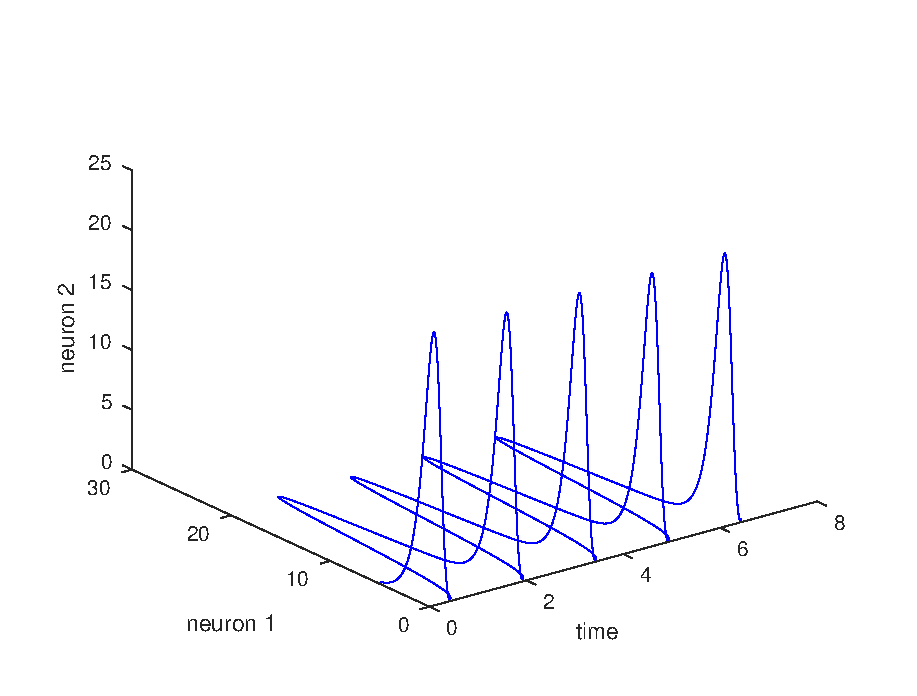
\includegraphics[width=\textwidth]{./images/SimFiringRate-with-time.eps}
           % 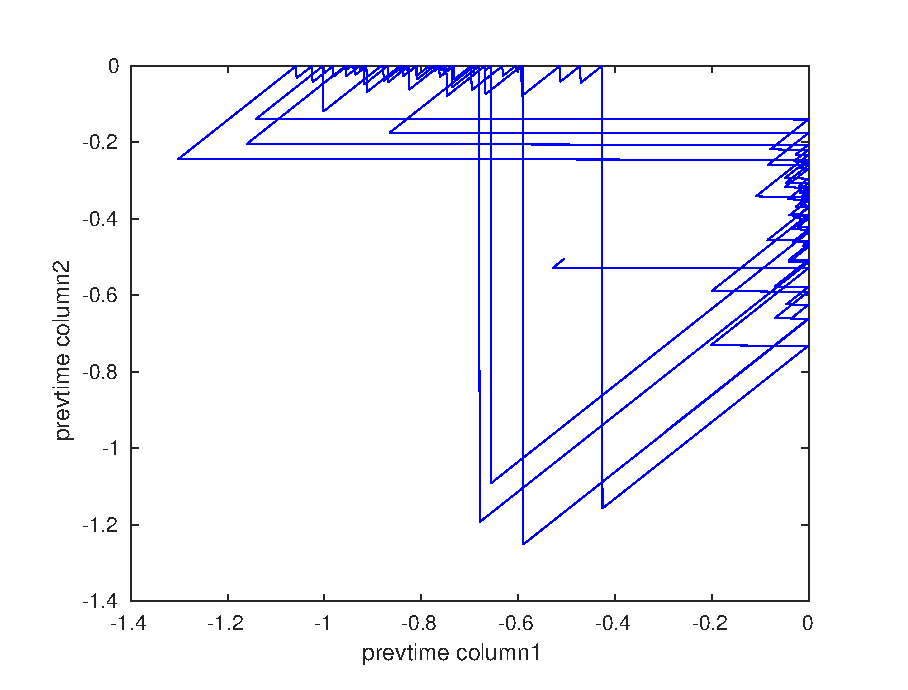
\includegraphics[width=\textwidth]{./images/FinalOralPlots/SyntheticOralPaper/SimPrevtime.eps}
            \caption[]%
            {{\small Simulated firing rate data (FR)}}  
            %{{\small Simulated previous time data (Prevtime)}} 
               
            \label{fig:Prevtime in 3D}
        \end{subfigure}
        \hfill
        % \vskip\baselineskip
        \begin{subfigure}[b]{0.475\textwidth}  
            \centering 
           % \includegraphics[width=\textwidth]{./images/FinalOralPlots/SyntheticOralPaper/SimFiringRate-with-Time.eps}
            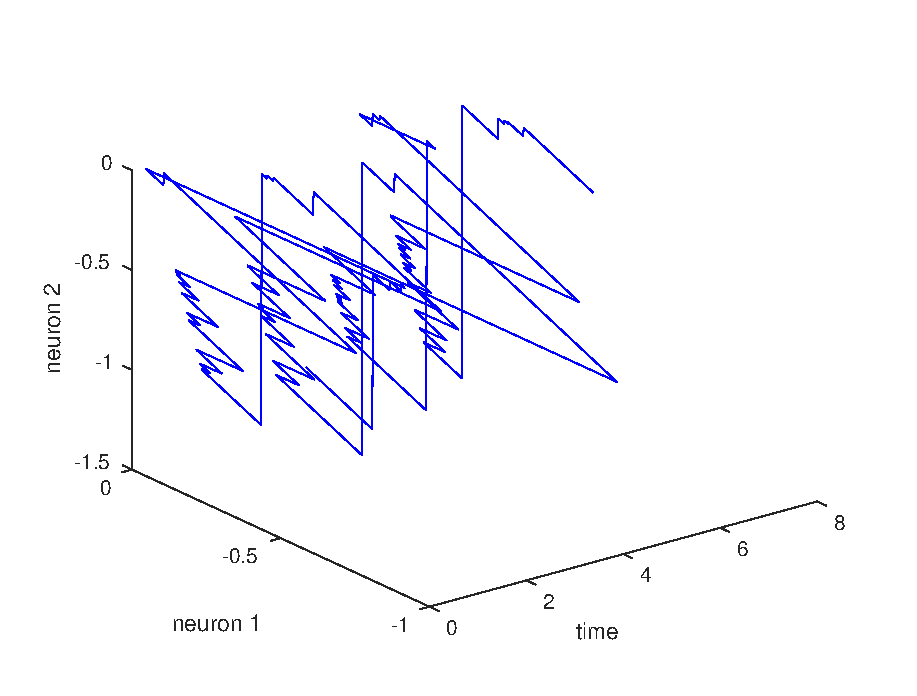
\includegraphics[width=\textwidth]{./images/SimPrevtime_with_time.eps}
            \caption[]%
            {{\small Simulated previous time data (Prevtime)}}  
            %{{\small Simulated firing rate data (FR)}}    
            \label{fig:Sim animal position in 3D}
        \end{subfigure}
        \caption[]%
         {\small  (a) Example of the firing rate of two neurons showing the modulation of the firing rates as the rat completes four and a half laps around a simulated circular track.
         (b) Example of the previous time of two neurons obtained after preprocessing  simulated spike times using  the 
         previous time measure. The pattern produced by the previous time measure is not clear in such a plot.} 
         
         \label{fig:Simulated_datasets}
\end{figure}
        
       
 
        
       \begin{figure}
       \centering
        \begin{subfigure}[b]{0.475\textwidth}   
            \centering 
            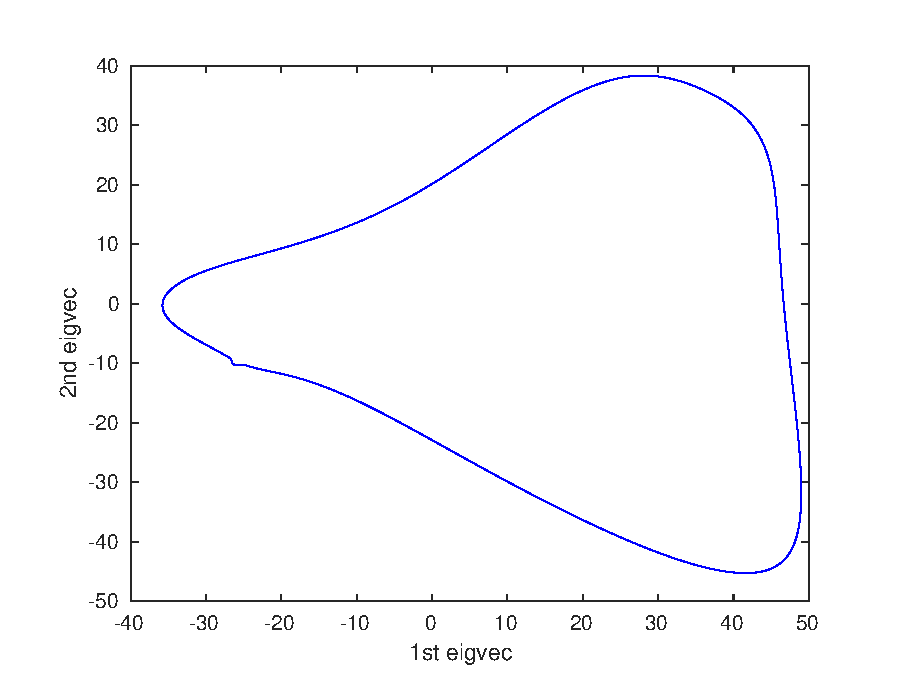
\includegraphics[width=\textwidth]{./images/FinalOralPlots/SyntheticOralPaper/SimFRPCA.eps}
           % 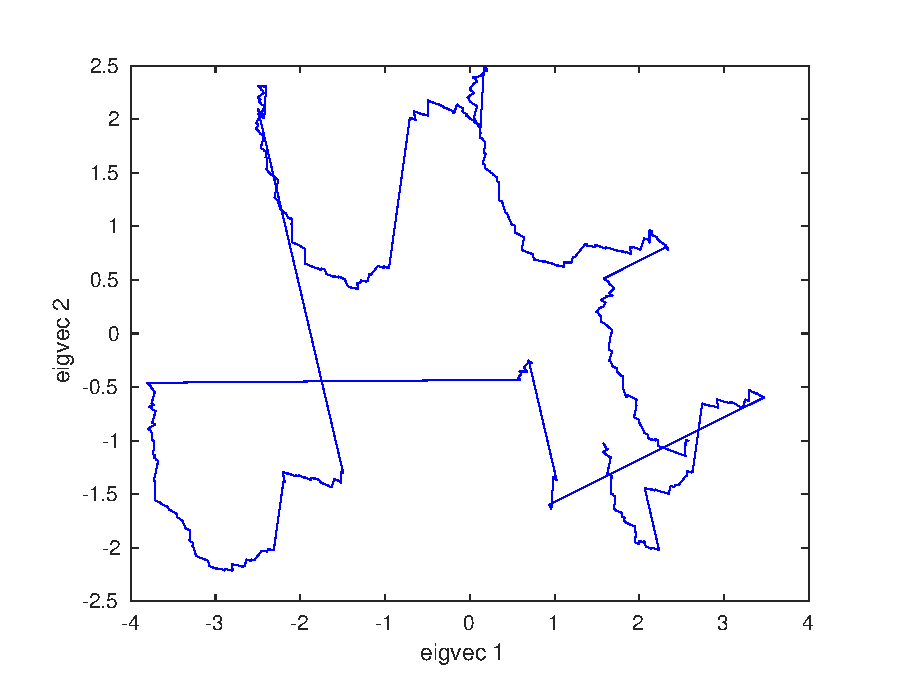
\includegraphics[width=\textwidth]{./images/FinalOralPlots/SyntheticOralPaper/SimPrevtimePCA.eps}
            \caption[]%
             {{\small PCA on FR}}   
            %{{\small PCA on Prevtime}}    
            \label{fig:PCA on Prevtime in 3D}
        \end{subfigure}
        \quad
        \begin{subfigure}[b]{0.475\textwidth}   
            \centering 
            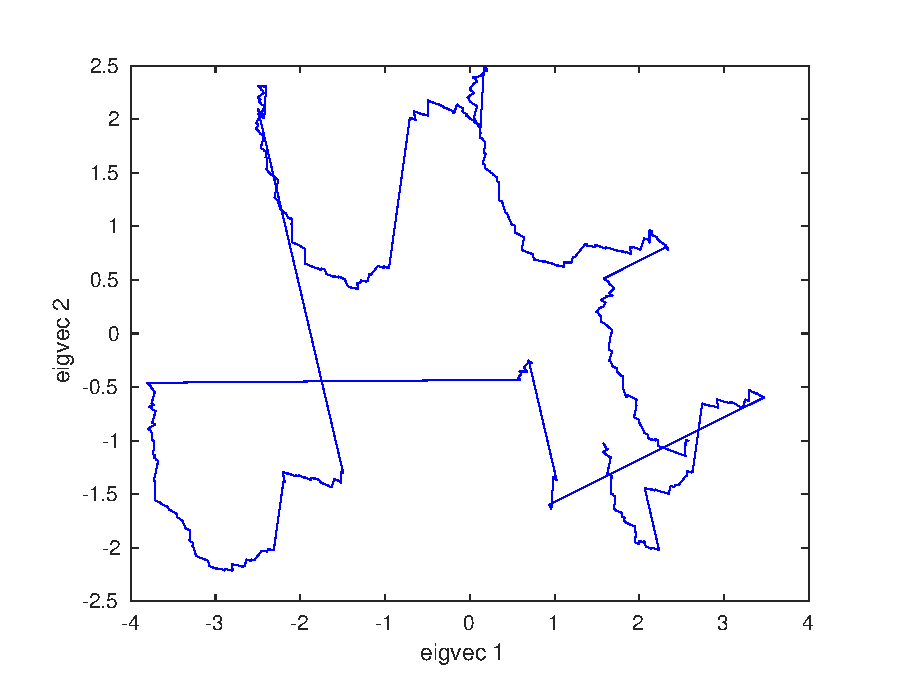
\includegraphics[width=\textwidth]{./images/FinalOralPlots/SyntheticOralPaper/SimPrevtimePCA.eps}
           % 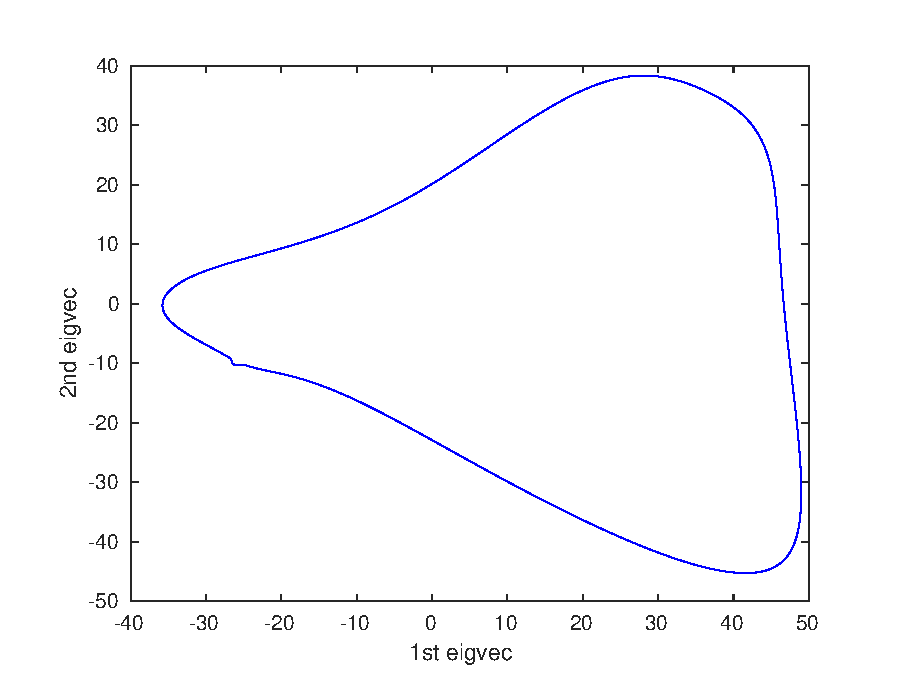
\includegraphics[width=\textwidth]{./images/FinalOralPlots/SyntheticOralPaper/SimFRPCA.eps}
            \caption[]%
             {{\small PCA on Prevtime}}   
           % {{\small PCA on FR}}    
            \label{fig:PCA on prevtime in 2D }
        \end{subfigure}
        \vskip\baselineskip
        \begin{subfigure}[b]{0.475\textwidth}   
            \centering 
             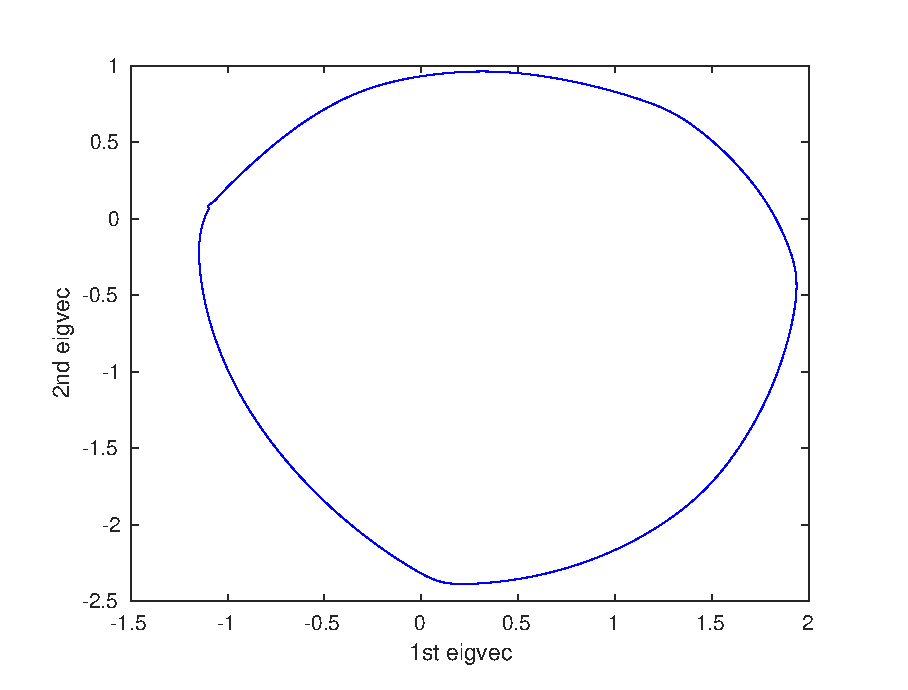
\includegraphics[width=\textwidth]{./images/FinalOralPlots/SyntheticOralPaper/SimFRDML1.eps}
          %  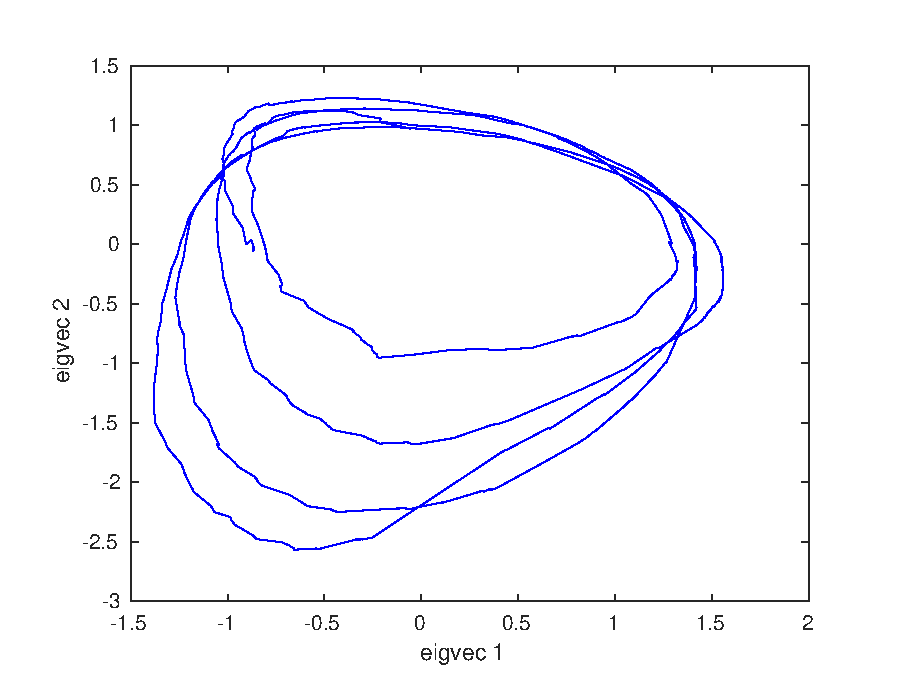
\includegraphics[width=\textwidth]{./images/FinalOralPlots/SyntheticOralPaper/SimPrevtimeDML1.eps}
            \caption[]%
             {{\small Diffusion Maps on FR}}    
            %{{\small Diffusion Maps on Prevtime}}    
            \label{fig:Diffusion maps on Prevtime in 3D}
        \end{subfigure}
        \quad
        \begin{subfigure}[b]{0.475\textwidth}   
            \centering 
             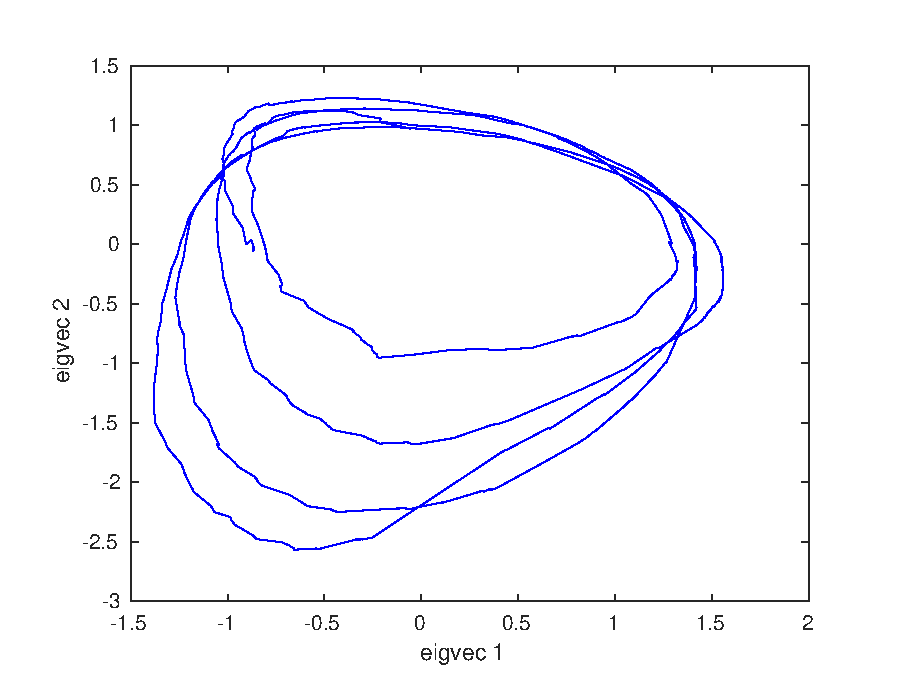
\includegraphics[width=\textwidth]{./images/FinalOralPlots/SyntheticOralPaper/SimPrevtimeDML1.eps}
           % 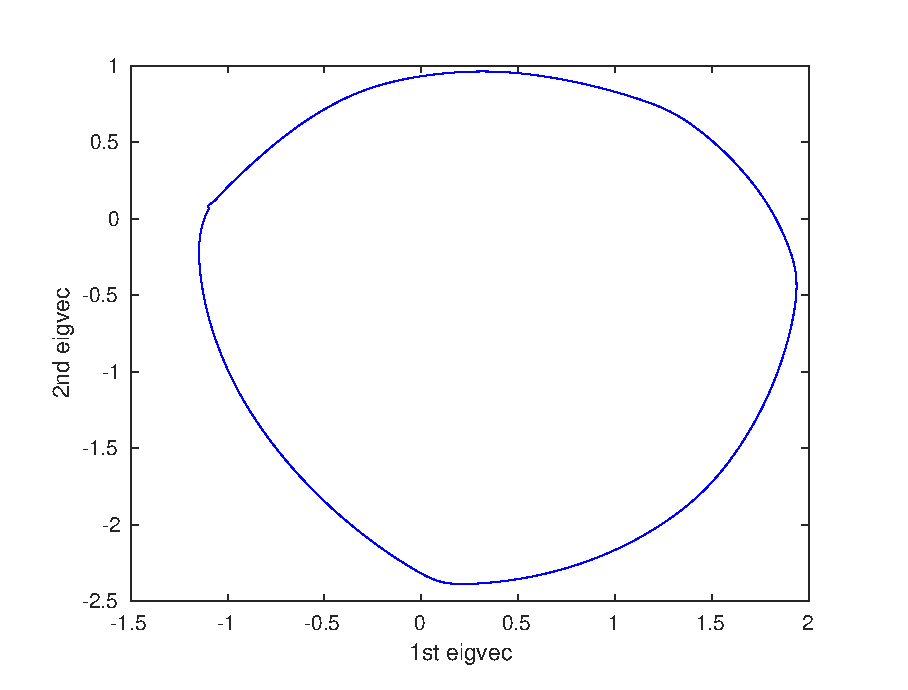
\includegraphics[width=\textwidth]{./images/FinalOralPlots/SyntheticOralPaper/SimFRDML1.eps}
            \caption[]%
            {{\small Diffusion Maps on Prevtime}}  
           % {{\small Diffusion Maps on FR}}    
            \label{fig:Diffusion maps on Prevtime in 3D }
        \end{subfigure}
        \caption[]%
         {\small Performance of PCA (first row) and Diffusion maps (second row) on simulated firing rate data (figure \ref{fig:Simulated_datasets} a),  and  previous  time data (figure \ref{fig:Simulated_datasets} b).
 A single point on any curve  represents the value of the first and second eigen vector at any time t.
(a, c) Each circle  corresponds to the four and a half laps made by the rat as the animal goes around a circular track. All the laps are superimposed on top of each other because the results in the left column are obtained after applying PCA  and Diffusion maps on clean firing rate data (with no noise). 
(b) Example showing that PCA applied to previous time data fails to reveal the four and a half laps taken by the rat around a circular track. 
(d)  Example showing that  Diffusion maps applied to previous time data recovers the four and a half laps taken by the rat around the circular  track. Since the rat's position in space is a circular curve parametrized in time, the top
         two eigen vectors of diffusion maps on previous time data capture the circular motion of the rat.} 
        \label{fig:DiffMaps_PCA_on_Prevtime_FR}
\end{figure}



\subsection{Interpretation of our results}
Analyzing synthetic spike time data preprocessed by the previous time measure captures the animal's position around the simulated circular track while using diffusion maps. We regard this observation as a potentially exciting area for future investigation since previous time data contains less information compared to using clean firing rate data. Even though we are using  synthetic data, these preliminary results show that pre-processing spike times using the previous time  measure should be explored in future analyses of real-world spike train data from the CA1 region of the rat hippocampus. 









%Our first step was to determine what dimensionality reduction algorithms to use.
%We decided to use Laplacian eigmaps \cite{belkin2003laplacian} and Diffusion Maps \cite{coifman2006} which are both non-linear dimensionality reduction algorithms.
%why?----to be addressed later.
%Initially, we smoothed the spike data using an exponential kernel defined by
%
%\[
%  K_{\tau}(t) =
%  \begin{cases}
%                 \frac{1}{\tau} \exp(-\frac{t}{\tau}) & \text{if $t > 0$} \\
%                  0 & \text{elsewhere} 
%  \end{cases}
%\]
%
%\subsection{Observations}
%We found that using Laplacian eigen maps to get an embedding based on the firing rate tried to
%recovered the position of the rat but could not reflect any variations along the path
%e.g the animal could have looked away from the track or run in a ragged fashion around the track.\\
%
%We also found that whenever there were gaps between the receptive fields (cases with no spikes),Laplacian Eigen Maps (LAM) performed poorly.
%This is because the nearest neighbor graph (based on the Euclidean distance used in (LAM) yields several connected components (i.e, the graph is disconnected).
%Since the eigen value decomposition step  in LAM is only applied on the largest connected
%component of the graph, the eigen vectors output by LAM are shorter than the total number of original data points (spike times). Thus the embedding provided by LAM is in accurate in some
%instances due to the "coverage" problem.\\
%
%Diffusion Maps (DM) algorithm tends to run out of memory in case of large instances
%so we were unable to compare the performance of both LAM and DM when using the firing rate.
%This is not true: First redo the analysis on sonet since you need to show that
%previous/next time is an improvement over the traditional firing rate.
%
%\subsection{Remedy for the coverage problem}
%Inspired by David Redish's idea, we decided to create previous and next time vectors which
%give us information even when there is no spike.
%This is the direction which seems promising at the moment since it tends to over come
%the problem of coverage. what is the coverage problem? (see reference on tunning curves).
%We then used the exponential kernel as our metric on the previous and next time data
%to generate a distance metric which is the main input in Diffusion Maps algorithm.
%
%
%
%
















































%\newpage

%%%%%%%%%%%%%%%%%%%%  Firing rate %%%%%%%%%%%%%%%%%%%%%%%%%%%%%%%%%%%%%%%%%%%%%%%%%%


%\begin{figure}[H]
%        \centering
%        \begin{subfigure}[b]{0.475\textwidth}
%            \centering
%            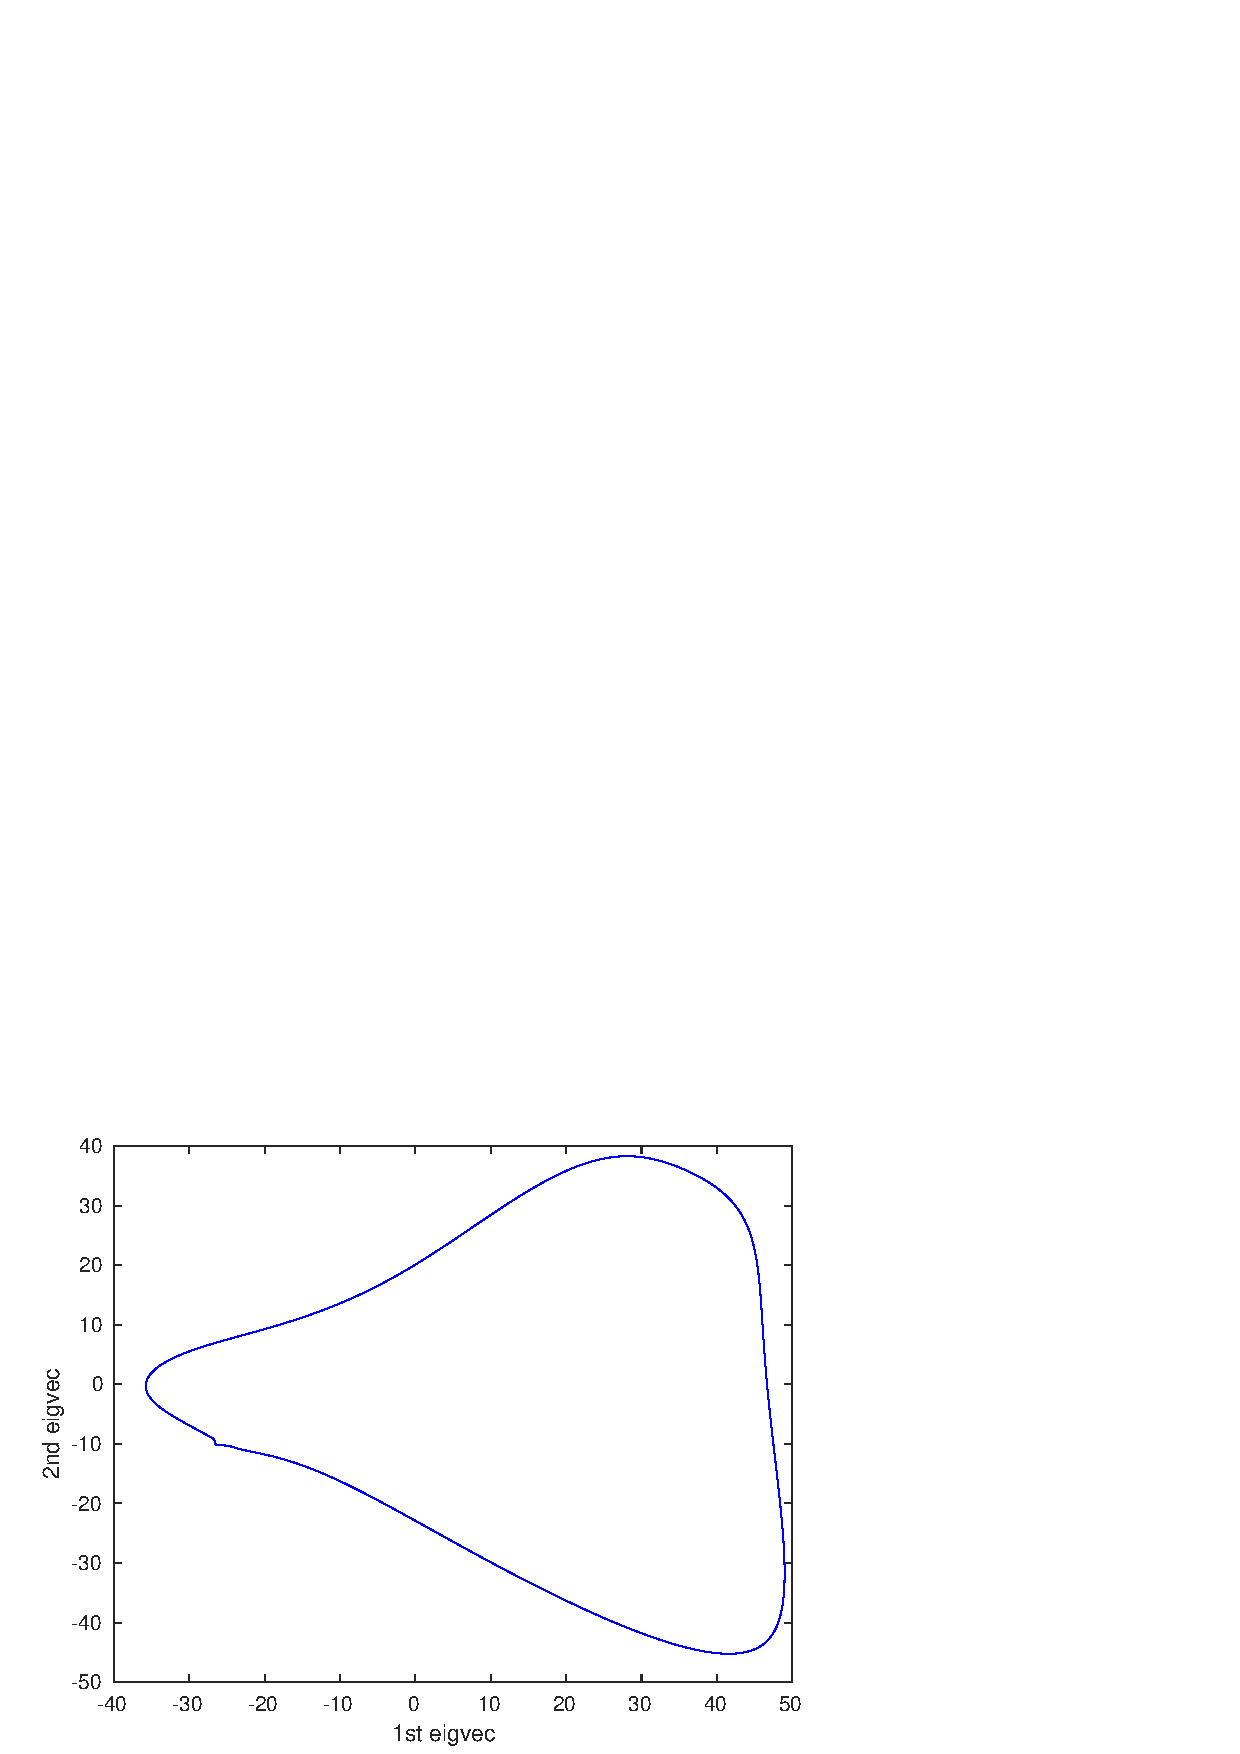
\includegraphics[width=\textwidth]{./images/FinalOralPlots/SyntheticOralPaper/SimFRPCA.pdf}
%            \caption[PCA on FR]%
%            {{\small PCA on FR}}    
%            \label{fig:PCA on FR in 3D}
%        \end{subfigure}
%        \hfill
%        \begin{subfigure}[b]{0.475\textwidth}  
%            \centering 
%            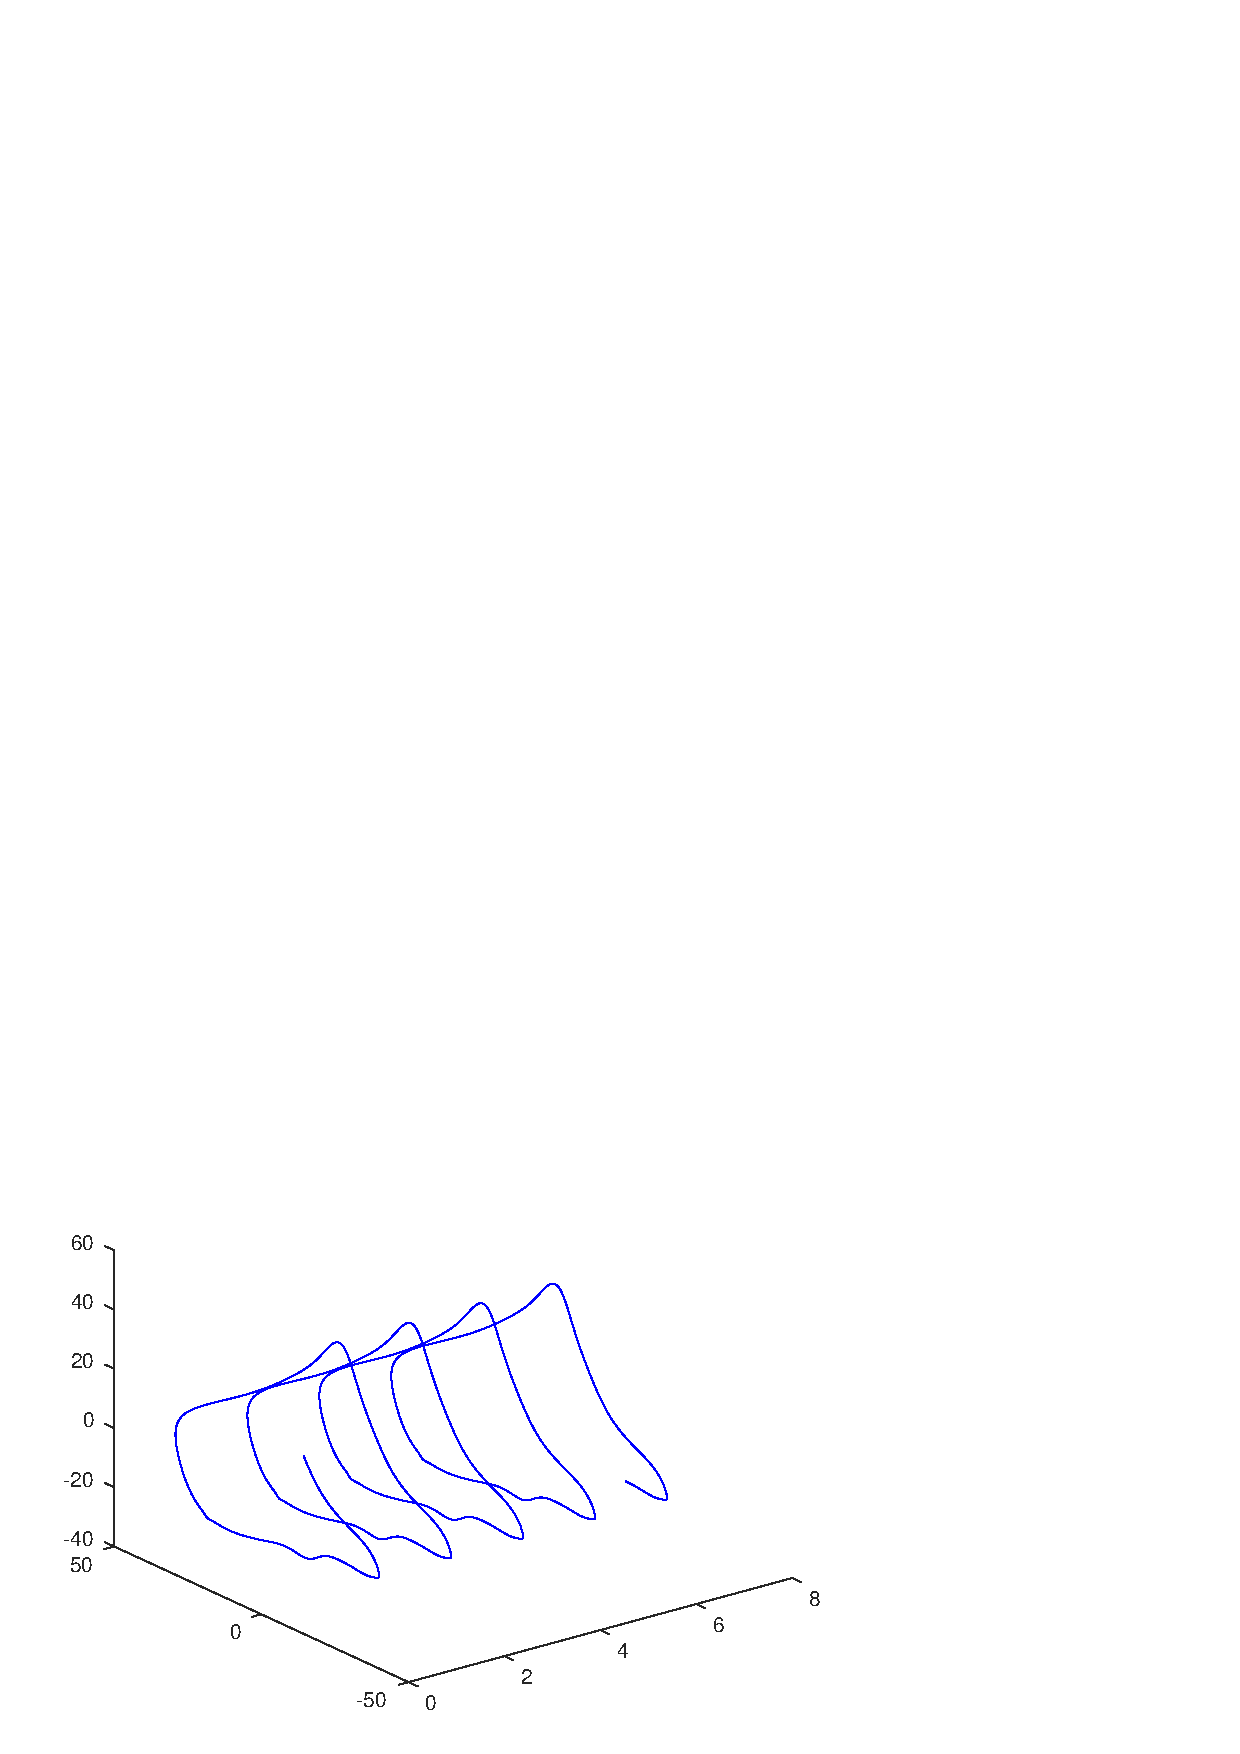
\includegraphics[width=\textwidth]{./images/FinalOralPlots/SyntheticOralPaper/SimFRPCA-with-time.pdf}
%            \caption[]%
%            {{\small PCA on FR}}    
%            \label{fig:PCA on FR in 2D}
%        \end{subfigure}
%        \vskip\baselineskip
%        \begin{subfigure}[b]{0.475\textwidth}   
%            \centering 
%            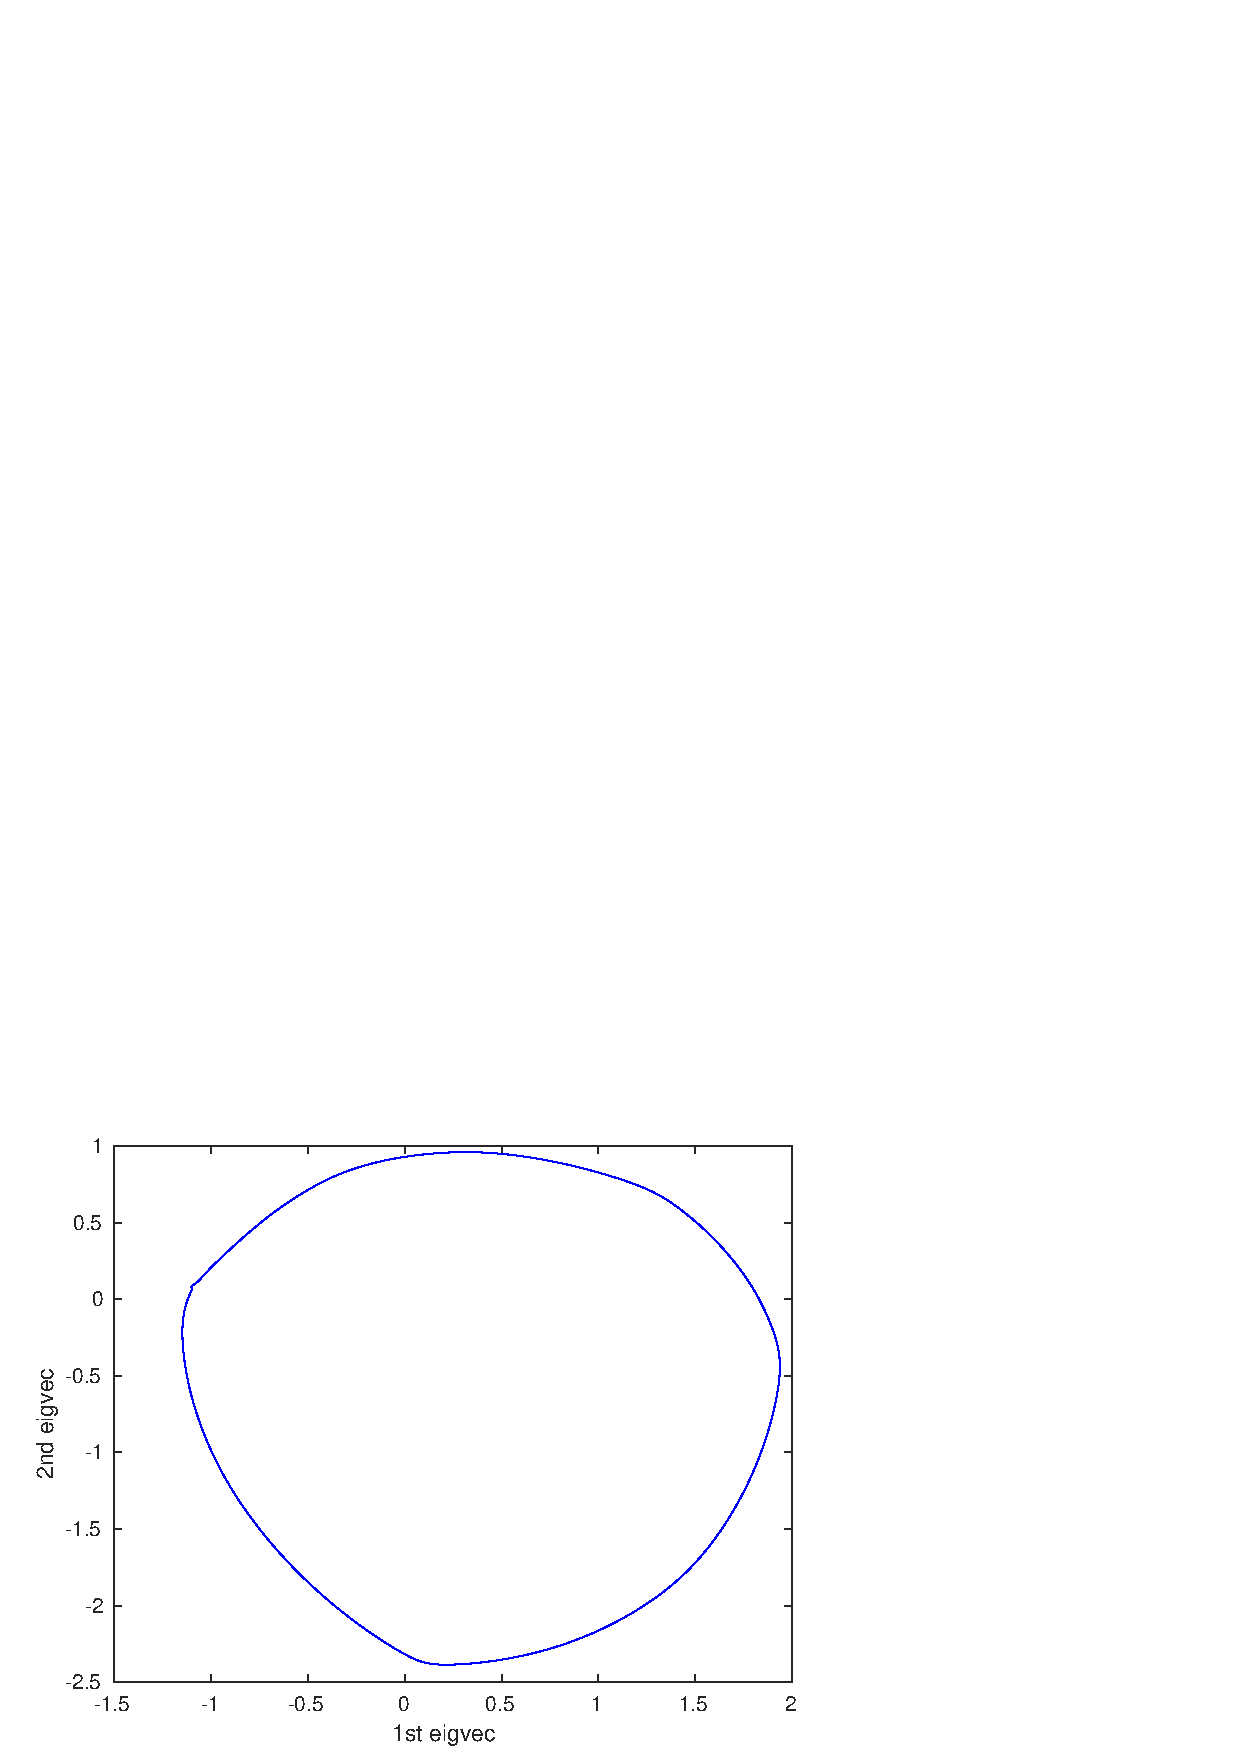
\includegraphics[width=\textwidth]{./images/FinalOralPlots/SyntheticOralPaper/SimFRDML1.pdf}
%            \caption[]%
%            {{\small Diffusion Maps on FR}}    
%            \label{fig:Diffusion maps on FR in 3D}
%        \end{subfigure}
%        \quad
%        \begin{subfigure}[b]{0.475\textwidth}   
%            \centering 
%            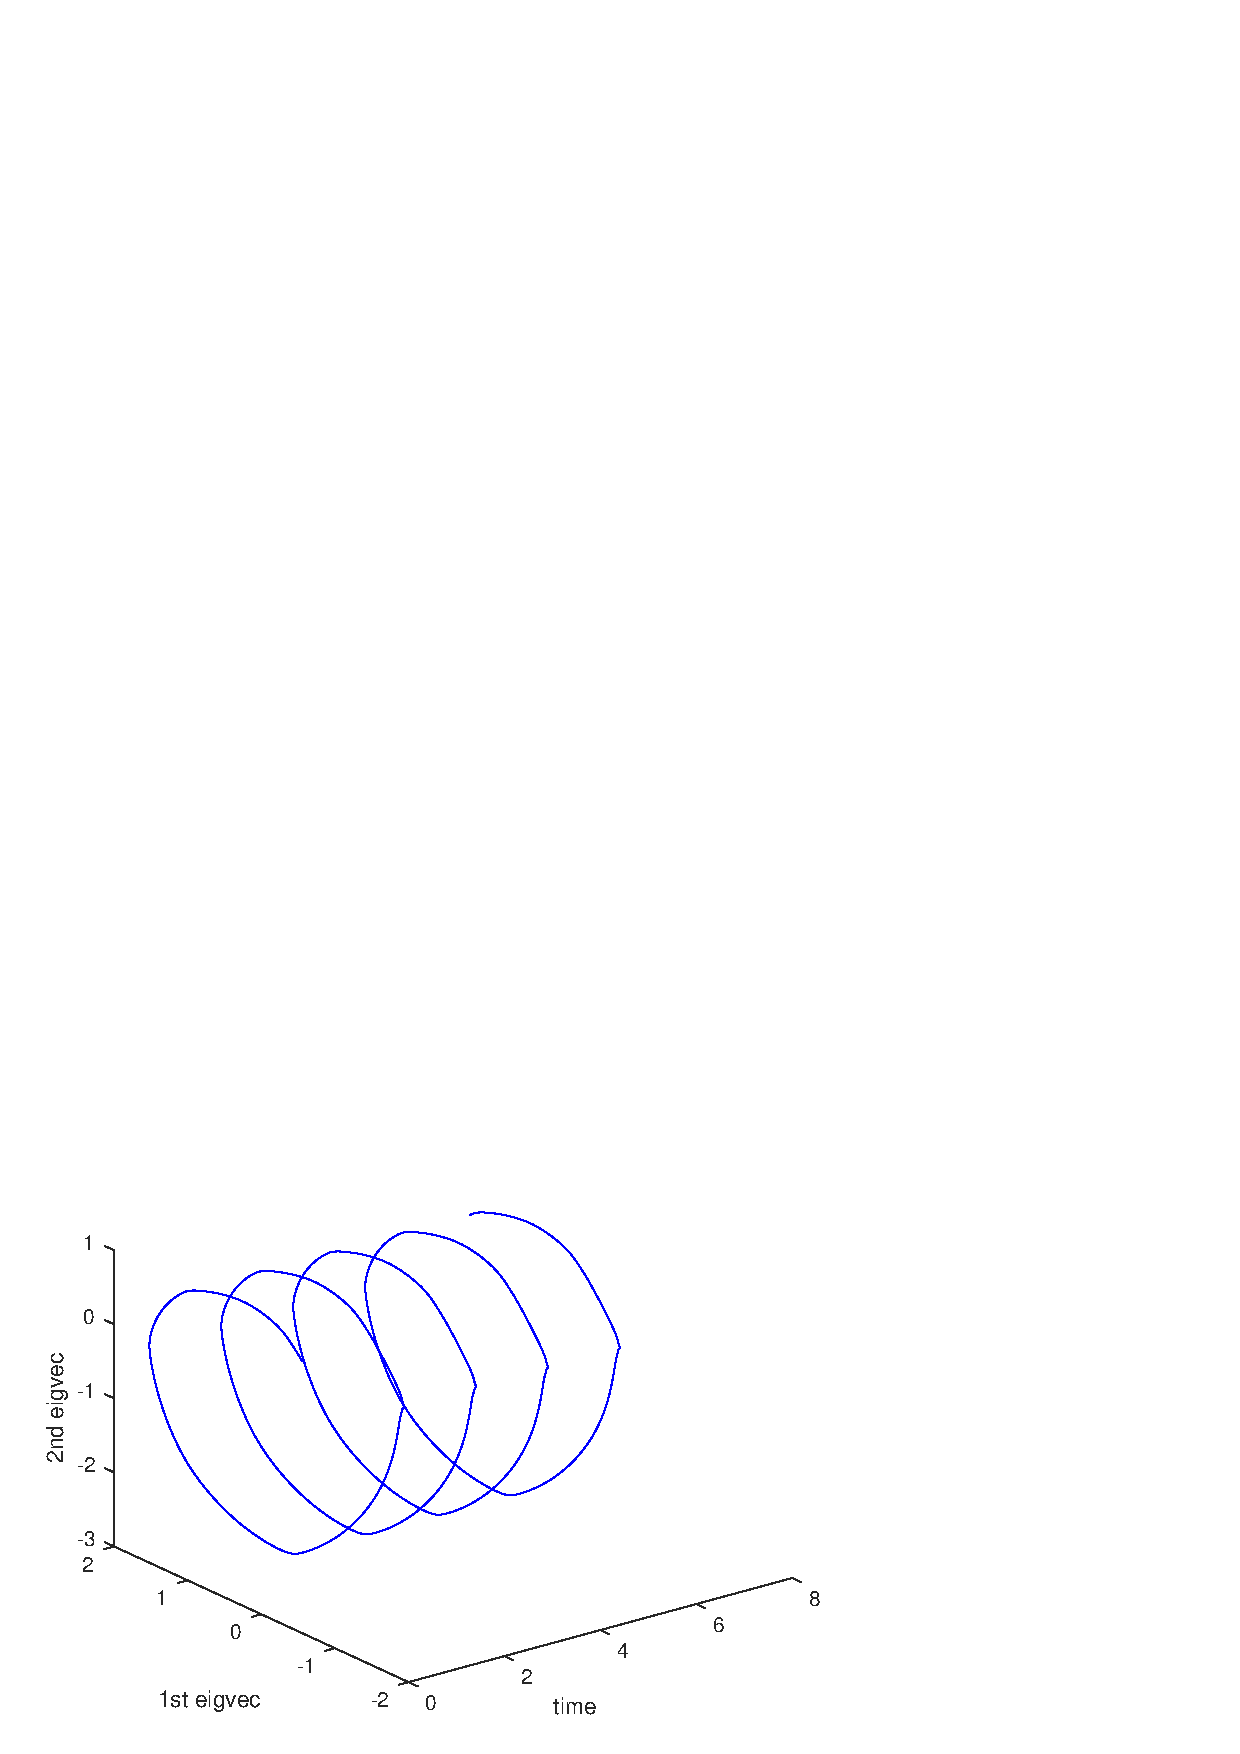
\includegraphics[width=\textwidth]{./images/FinalOralPlots/SyntheticOralPaper/SimFRDML1-with-time.pdf}
%            \caption[]%
%            {{\small Diffusion Maps on FR}}    
%            \label{fig:Diffusion maps on FR in 2D }
%        \end{subfigure}
%        \caption[small Performance of Diffusion maps and PCA on simulated firing rate data ]
%        {\small Performance of Diffusion maps and PCA on simulated firing rate data} 
%        \label{fig:DiffMaps_PCA_on_FR}
%    \end{figure}
%
%


%Next, we show the results of diffusion maps with $l_{1}$ distance 
%and PCA on simulated previous time data (Prevtime). 

%%%%%%%%%%%%%%%%%%%%%%%%%%%% Prevtime and simulated position %%%%%%%%%%%%%%%%%%%%%%%%%%%%%

%\begin{figure}[H]
%        \centering
%        \begin{subfigure}[b]{0.475\textwidth}
%            \centering
%            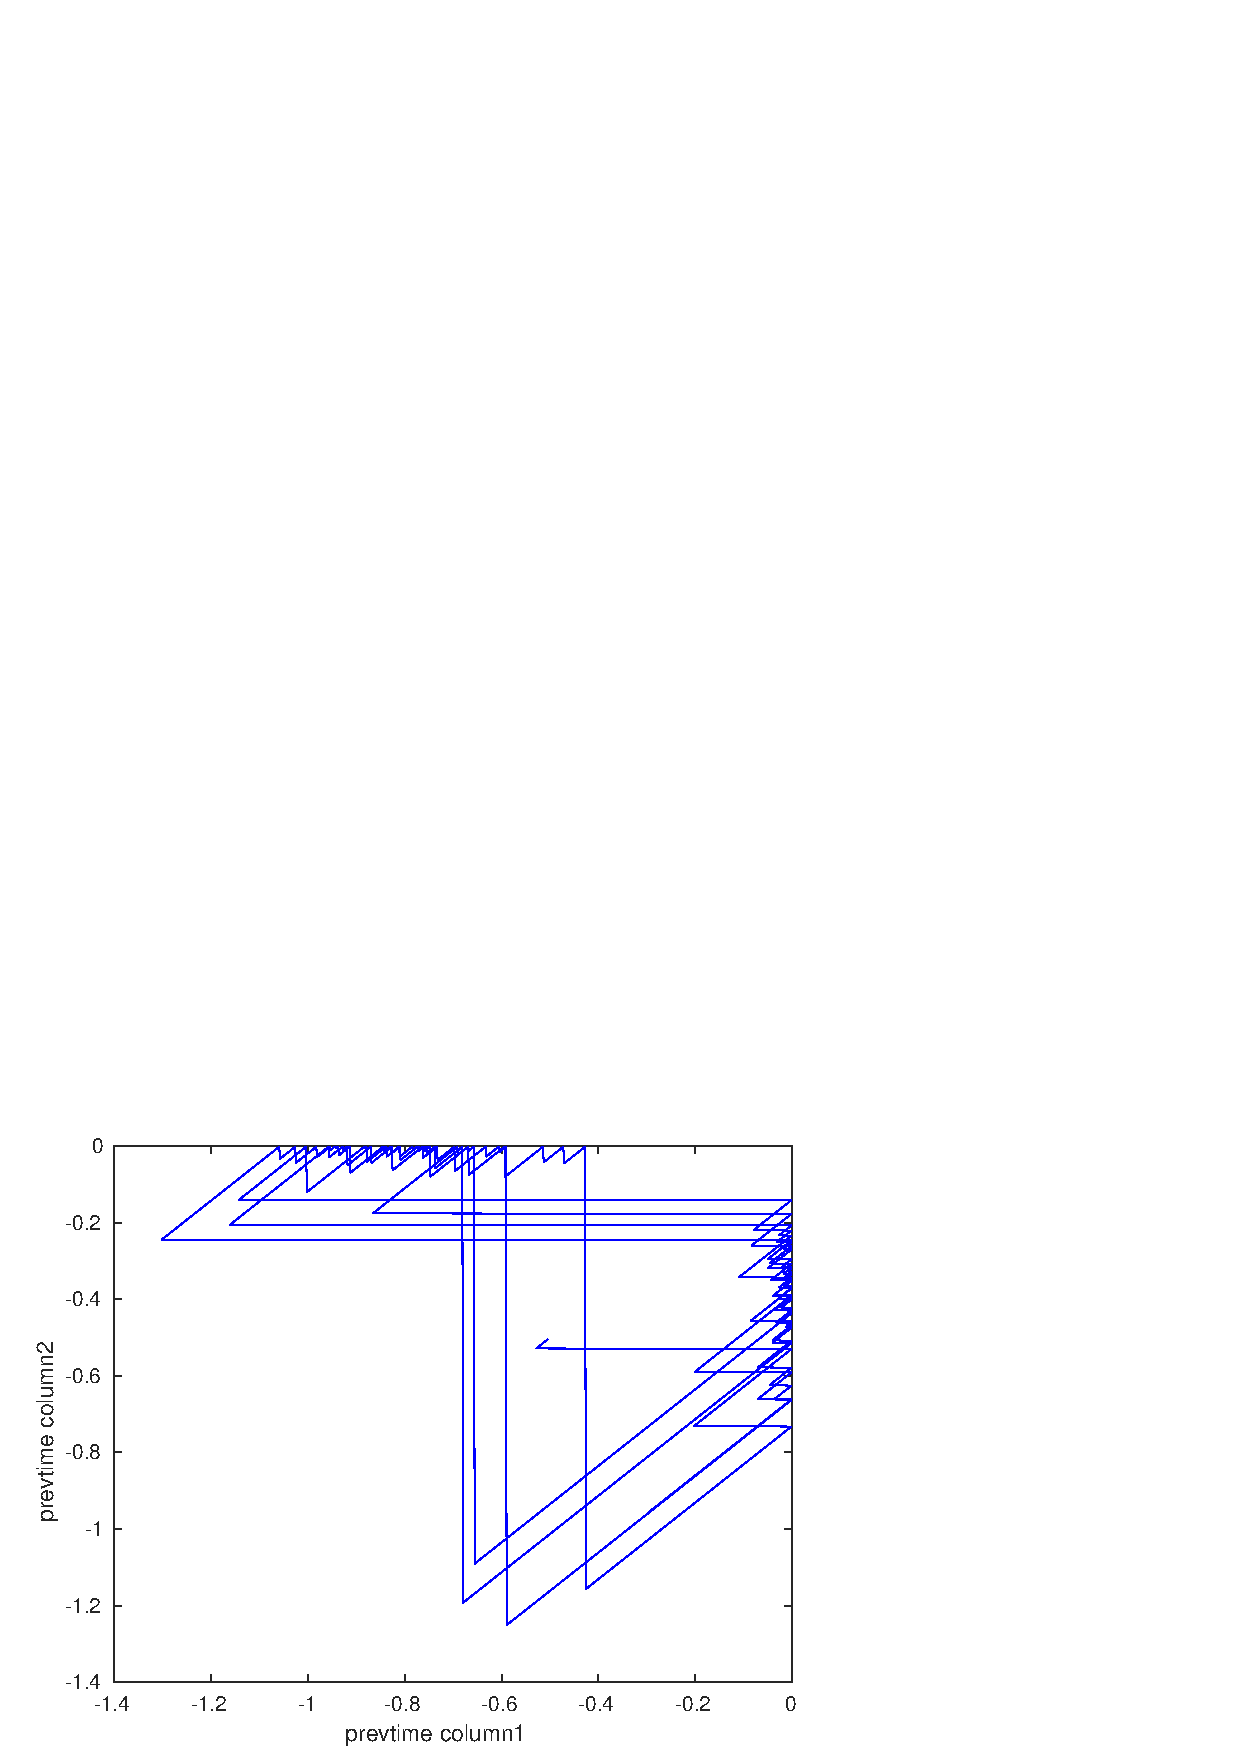
\includegraphics[width=\textwidth]{./images/FinalOralPlots/SyntheticOralPaper/SimPrevtime.pdf}
%            \caption[Simulated Prevtime]%
%            {{\small Simulated Prevtime}}    
%            \label{fig:Prevtime in 3D}
%        \end{subfigure}
%        \hfill
%        \begin{subfigure}[b]{0.475\textwidth}  
%            \centering 
%            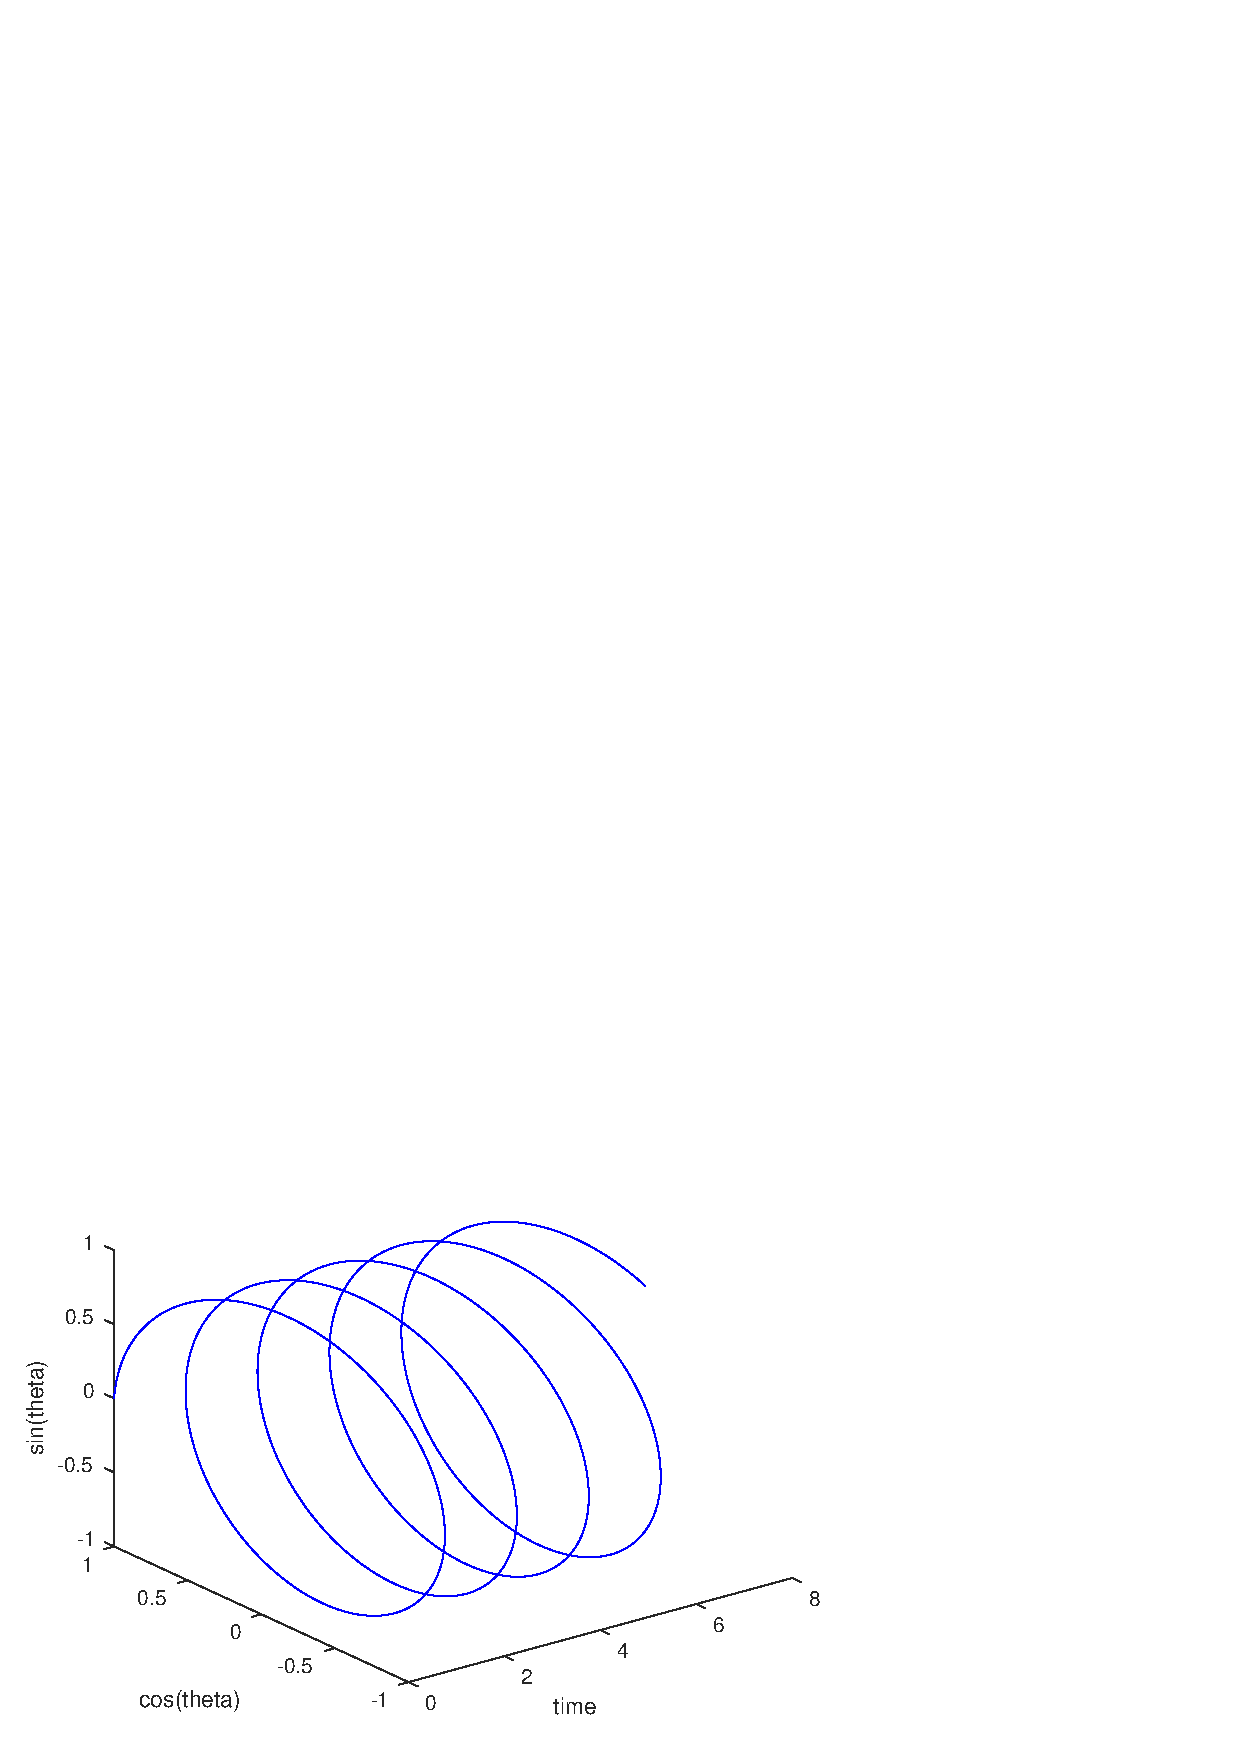
\includegraphics[width=\textwidth]{./images/FinalOralPlots/SyntheticOralPaper/SimRatPosition.pdf}
%            \caption[]%
%            {{\small Simulated animal position}}    
%            \label{fig:Sim animal position in 3D}
%        \end{subfigure}
%        \vskip\baselineskip
%        \begin{subfigure}[b]{0.475\textwidth}   
%            \centering 
%            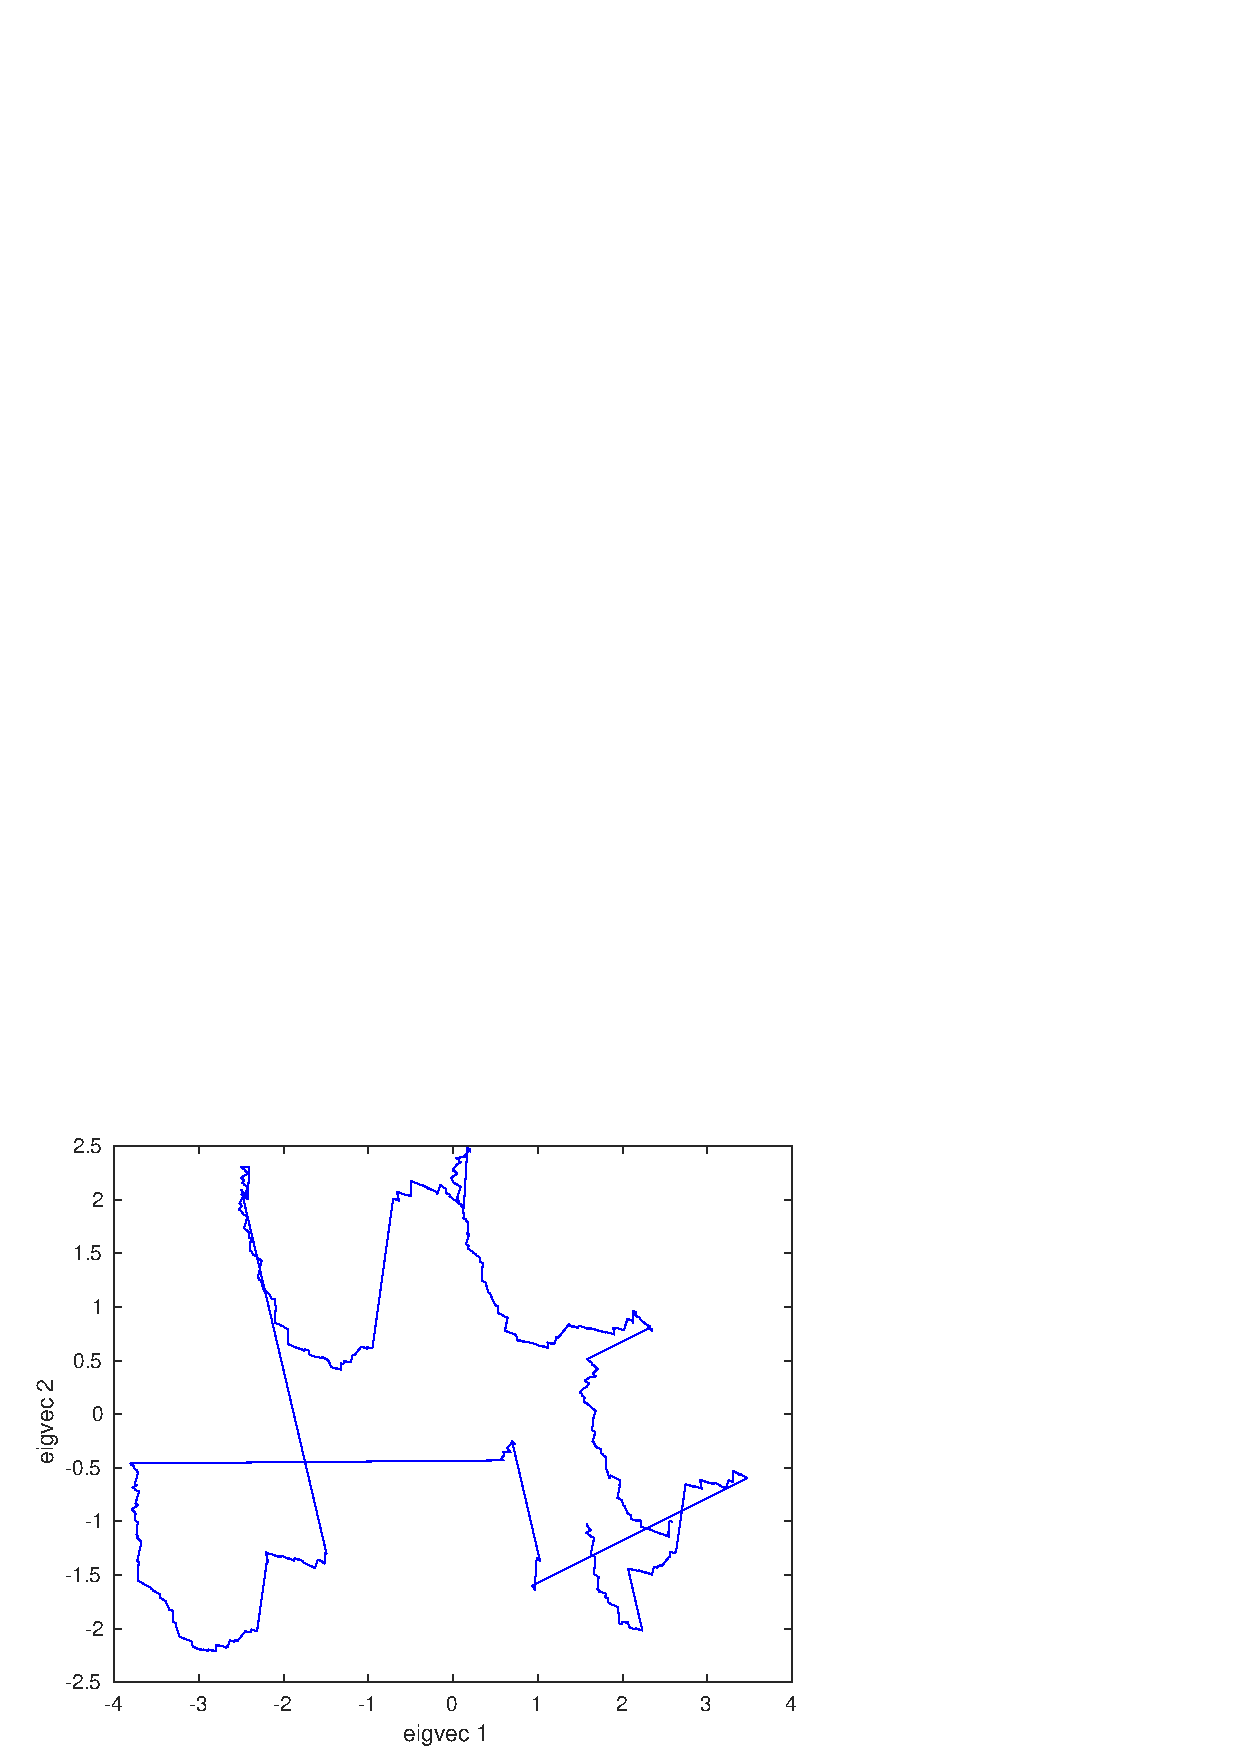
\includegraphics[width=\textwidth]{./images/FinalOralPlots/SyntheticOralPaper/SimPrevtimePCA.pdf}
%            \caption[]%
%            {{\small PCA on Prevtime}}    
%            \label{fig:PCA on Prevtime in 3D}
%        \end{subfigure}
%        \quad
%        \begin{subfigure}[b]{0.475\textwidth}   
%            \centering 
%            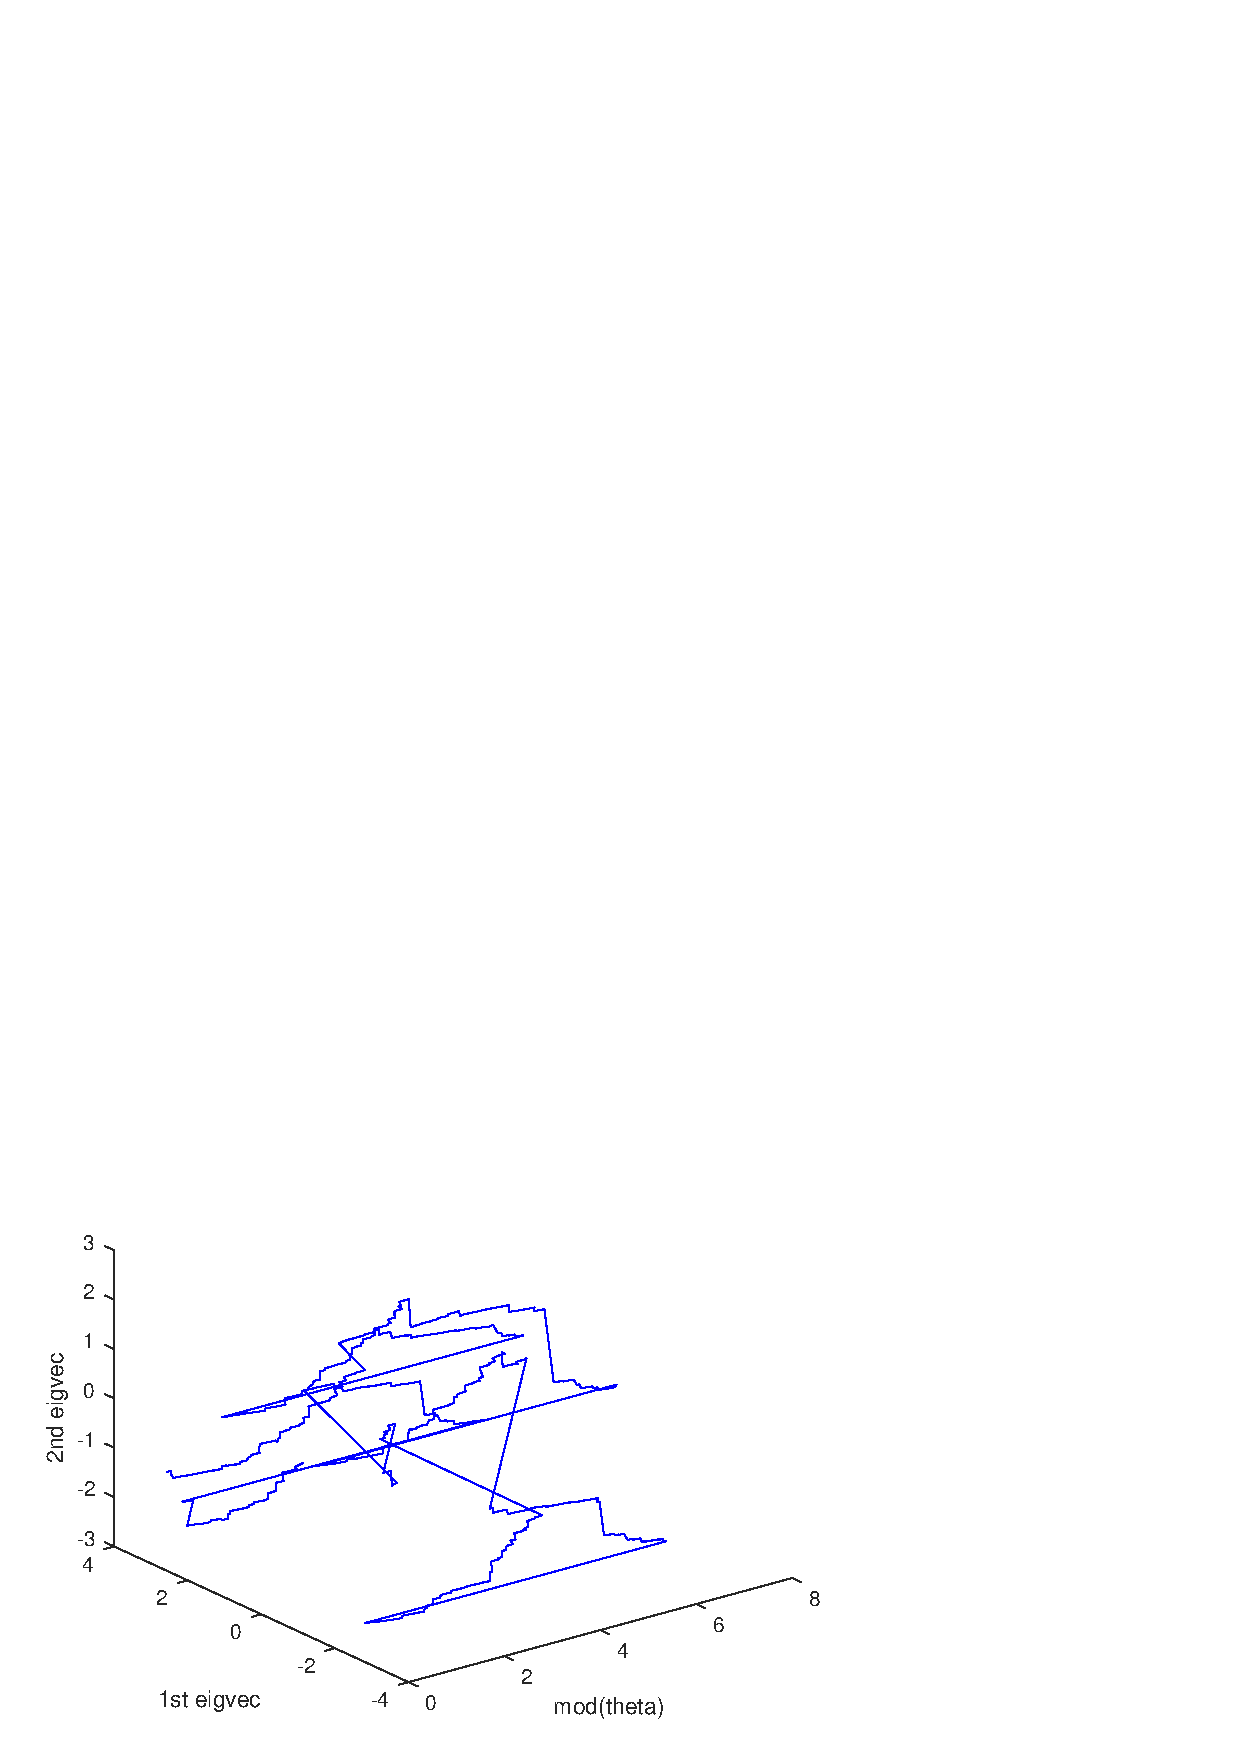
\includegraphics[width=\textwidth]{./images/FinalOralPlots/SyntheticOralPaper/SimPrevtimePCA-with-Position.pdf}
%            \caption[]%
%            {{\small PCA on prevtime}}    
%            \label{fig:PCA on prevtime in 2D }
%        \end{subfigure}
%        \vskip\baselineskip
%        \begin{subfigure}[b]{0.475\textwidth}   
%            \centering 
%            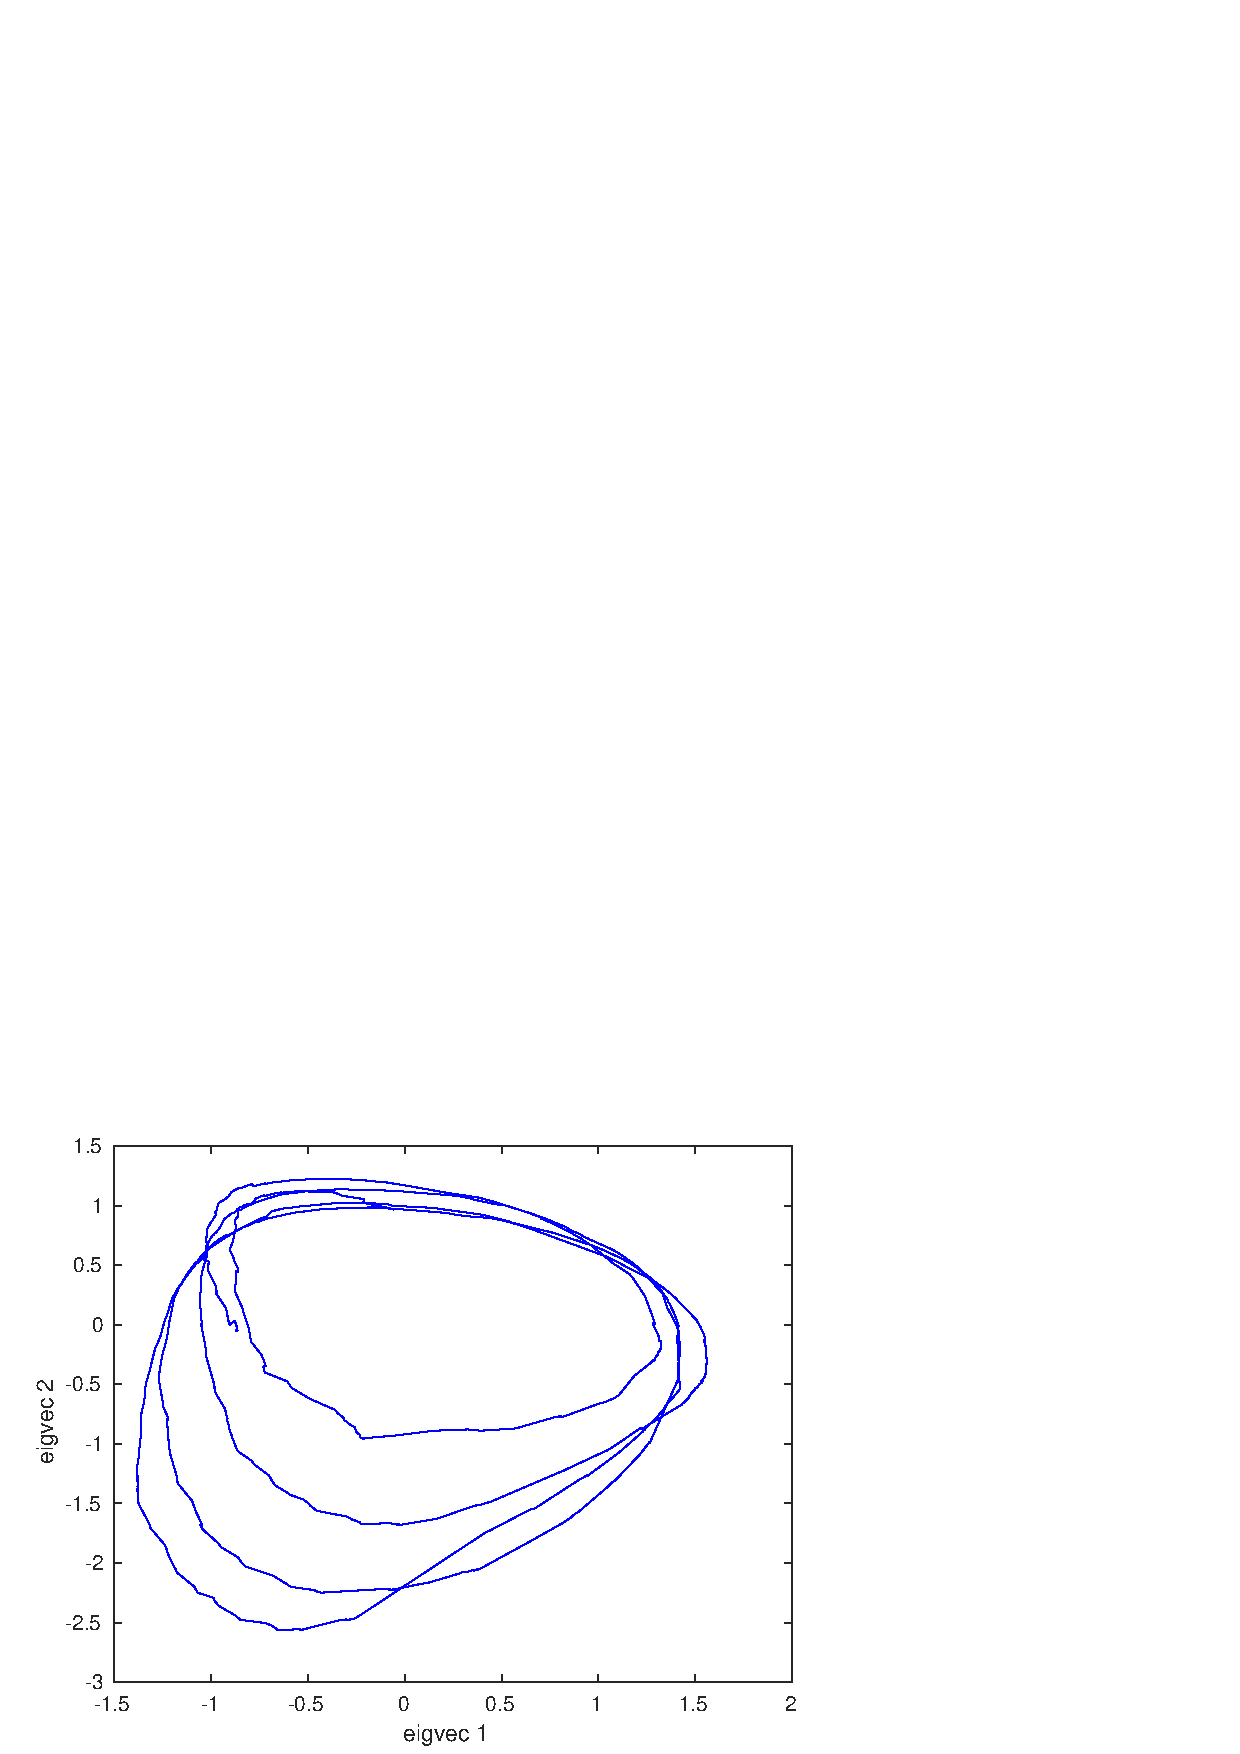
\includegraphics[width=\textwidth]{./images/FinalOralPlots/SyntheticOralPaper/SimPrevtimeDML1.pdf}
%            \caption[]%
%            {{\small Diffusion Maps on Prevtime}}    
%            \label{fig:Diffusion maps on Prevtime in 3D}
%        \end{subfigure}
%        \quad
%        \begin{subfigure}[b]{0.475\textwidth}   
%            \centering 
%            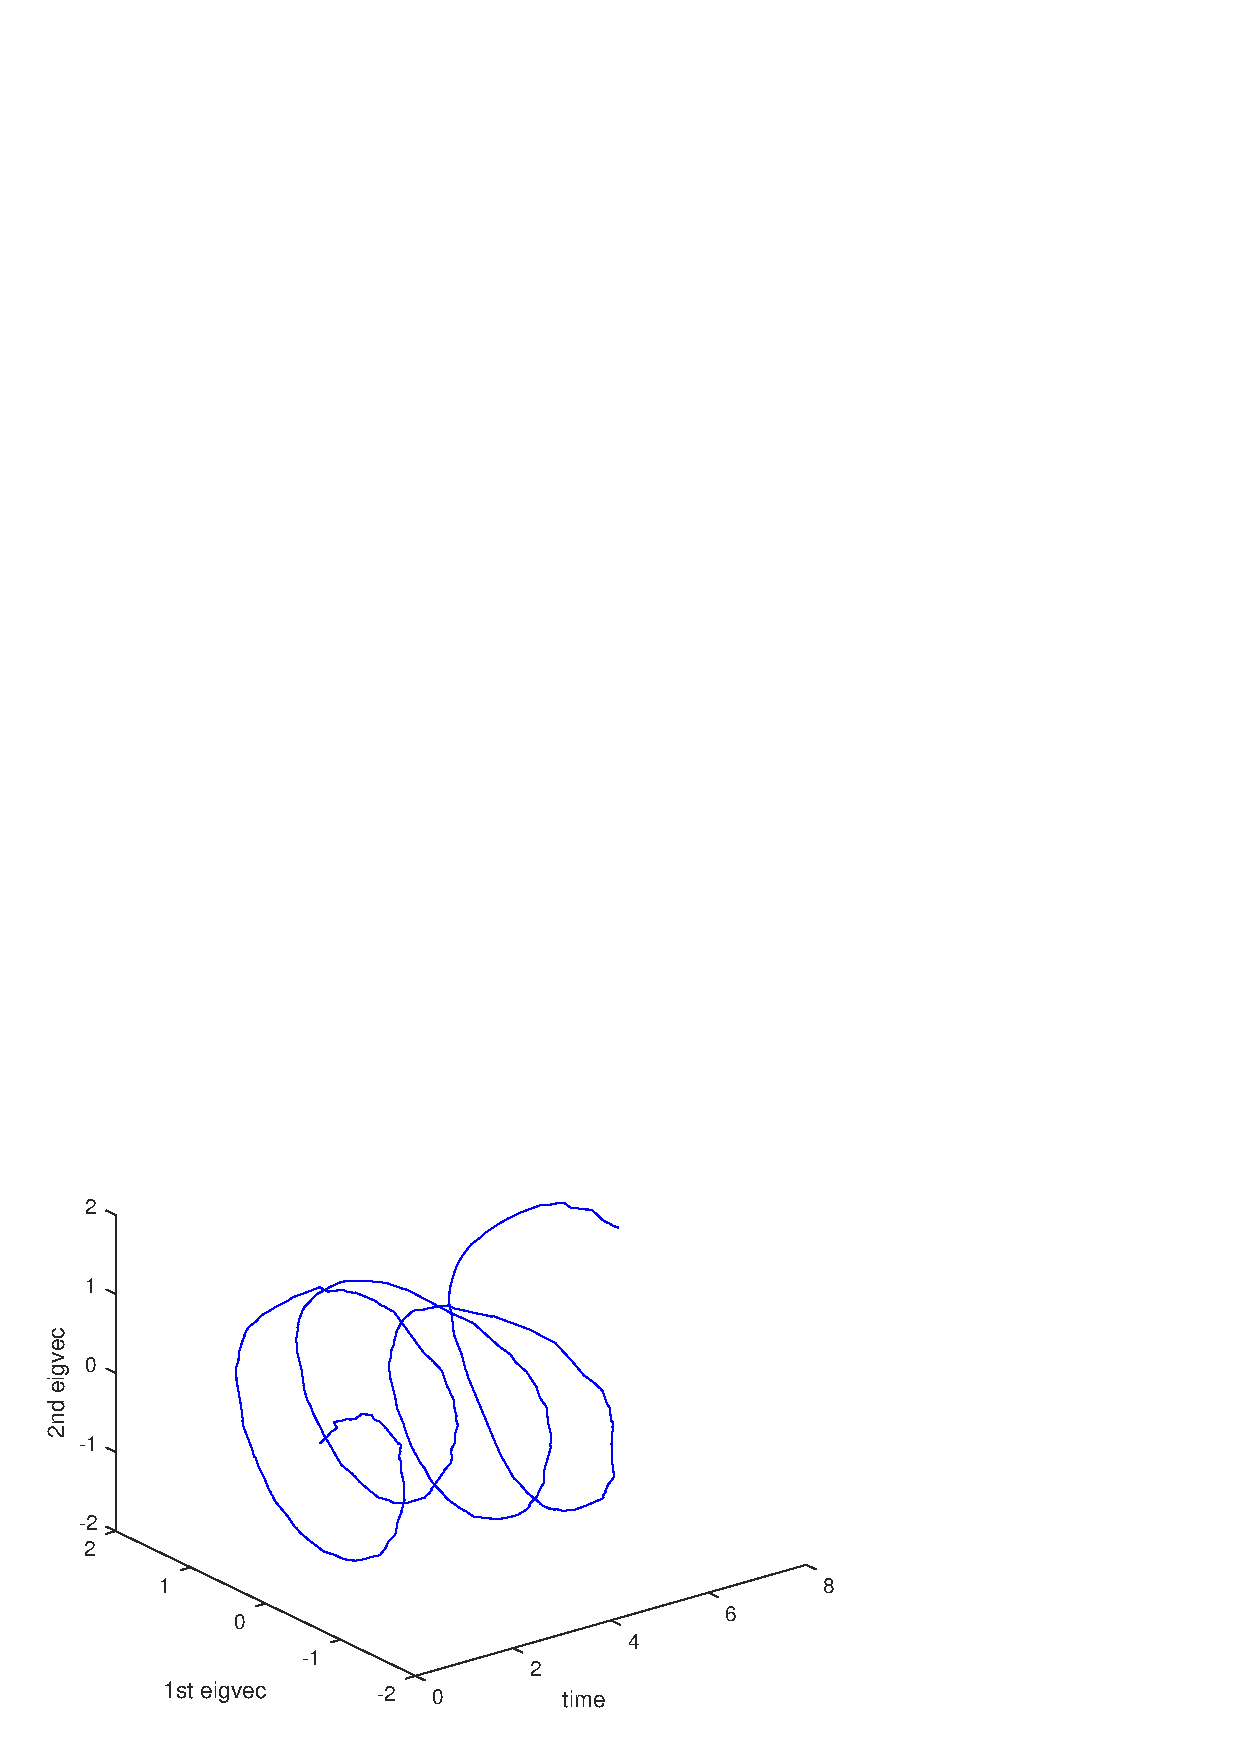
\includegraphics[width=\textwidth]{./images/FinalOralPlots/SyntheticOralPaper/SimPrevtimeDML1-with-Position.pdf}
%            \caption[]%
%            {{\small Diffusion Maps on Prevtime}}    
%            \label{fig:Diffusion maps on Prevtime in 3D }
%        \end{subfigure}
%        \caption[Performance of Diffusion maps and PCA on simulated previous time data ]
%        {\small Performance of Diffusion maps and PCA on simulated previous time data} 
%        \label{fig:DiffMaps_PCA_on_Prevtime}
%\end{figure}
%


















 































































%\begin{itemize}
%\item show the graphs/results package
%\item this is how we're interpreting the results
%\item why does this matter?
%\item what measure of goodness did you use?
%(Fisher Vs Shannon information)

%%==========suggested by Duane============================================
%\item Mention that there are other ways of checking measures of goodness
% e.g the one provided by diffusion maps, Bayesian decoding refer to the nature
% and review artcicle.


%\end{itemize}








%
%
\input{chapters/future_direction}
%
%
%\mychapter{8}{Future work}


%%%%%%%%%%%%%%%% Generate a Bibliography%%%%%%%%%%%%%%%%%%%%%%%%%%%%%%%%%%%%%%%%
%%==== put the bibliography after all sections=====
% but above end document===========================
\pagebreak

%add a bibliography using mendeley

\bibliography{./References/library.bib}

\bibliographystyle{unsrt}


\pagebreak


\appendix
\begin{appendices}
\section{Linear algebra review}\label{SVD}
\subsection{Definitions}


\begin{Def}
An $n\times n$ symmetric matrix $\Bm{A}$ is positive semidefinite (PSD) if the quadratic form
\[
\vect{x} \Bm{A} \vect{x}^{\top} \geq 0,\ \ \text{for all non-zero vectors} \ \ \vect{x} \in \R^{n}
\]

Given any $n\times n$ matrix $\Bm{A}$, the matrices $\Bm{A}\Bm{A}^{\top}$
and $\Bm{A}^{\top}\Bm{A}$ are symmetric PSD.

\end{Def}

\begin{Def}
Let $\R^{n \times m}$ denote the vector space of $n \times m$ matrices with real entries. Given any $n\times m$ matrix $\bm{A}$ with real entries, there exist orthonormal matrices $\bm{U} \in \R^{n \times n}$ and $\bm{V} \in \R^{m \times m}$ such that 
$\bm{\displaystyle A = U \Sigma V^{\top}}$ with $\bm{\Sigma}$ = \text{diag}$(\sigma_{1}, \ldots, \sigma_{k})$ where  k = $\min(n, m)$ and
 $\sigma_{1} \geq \sigma_{2} \geq \ldots \geq \sigma_{k} \geq 0$.
The numbers $\sigma_{i}, 1\leq i\leq n$ are called the singular values of $\bm{A}$. 
\end{Def}


\subsection{Properties of SVD}
Given any $n\times m$ real matrix $A$ of rank $r$, there exist matrices  $\bm{U} \in \R^{n \times r}$ and $\bm{V} \in \R^{r \times r}$ satisfying $\bm{U^{\top}U = V^{\top}V = I}$ such that $\bm{\text{A} = \text{U} \Sigma_{1} \text{V}^{\top}}$ with $\bm{\Sigma}_{1}$ = \text{diag}$(\sigma_{1}, \ldots, \sigma_{r})$ and $\sigma_{1} \geq \sigma_{2} \geq \ldots \geq \sigma_{r} > 0$.
This factorization of $\bm{A}$ is called the truncated SVD of $A$.
The rank of $A$ is equal to the number of non-zero singular values of $A$.
If $\bm{U}$ and $\bm{V}$ are made up of column vectors so that  $\bm{U} = [\vect{u}_1, \ldots, \vect{u}_{r}]$ and $\bm{V} = [\vect{v}_{1}, \ldots, \vect{v}_{r}]$ then $\{ \vect{u}_1, \ldots, \vect{u}_{r} \}$  and $\{\vect{v}_{1}, \ldots, \vect{v}_{r} \}$ are called the left and right singular vectors of $A$ respectively. \\
The matrix $A$ admits the SVD expansion 
\[
A = \sum_{i=1}^{r} \sigma_{i} \vect{u}_{i} \vect{v}_{i}^{\top}.
\]
The real numbers $\{\lambda_{1}, \ldots, \lambda_{r}\}$ where $\lambda_{i} = \sigma_{i}^{2}$ for all i = $1 , \ldots, r$ are the non-zero eigenvalues of both symmetric matrices $\bm{A^{\top}A}$ and $\bm{AA^{\top}}.$ The right singular vectors of $\bm{A}$ are the eigenvectors of $\bm{A^{\top}A}.$ The left singular vectors of $\bm{A}$ are the eigenvectors of $\bm{AA^{\top}}.$ The spectral decomposition of $\bm{A^{\top}A}$ is given by $\bm{A^{\top}A  = V D_{1} V^{\top}}$ and that of  $\bm{AA^{\top}}$ is given by  $\bm{AA^{\top}} = U D_{2} U^{\top}$ where $\bm{U}$ and $\bm{V}$ are the SVD factors upto a sign, $\bm{D}_{1}$ and $\bm{D}_{2}$ are diagonal matrices containing the r singular values of $A$.


\section{Proximity measures}\label{proximity}

\begin{Def}
A proximity measure characterizes how close two objects are, using
either a similarity or dissimilarity measure between them \cite{CoxT2000}.
A similarity measure characterizes how similar two objects are while
a dissimilarity measure or distance characterizes how dissimilar two objects are.
\end{Def}


\begin{Def}\label{distance}
Let $X$ be a set of $n$ objects, $\{x_{1}, \dots, x_{n}\}$, that are not necessarily vectors. A distance, $d$, on $X$, is a real-valued  function
$d: X \times X \rightarrow  \R$ which assigns to each pair of objects, (x$_{i}$, x$_{j}$), a real number, $d_{ij}$, satisfying two conditions, for all $i$ and $j$ from 1 to $n$. 
\begin{itemize}
\item [i)] $d_{ij} \geq 0$ and $d_{ij} = 0$ if and only if $i=j$
\item [ii)] $d_{ij} = d_{ji}$
\end{itemize}
\end{Def}


A metric is a distance function, $d$, which satisfies the triangle inequality:
$d_{jk} \leq d_{ij} + d_{ik}, \ \ \text{for all}\ \ i,j,k$ 


\begin{Def}
A similarity measure $s: X \times X \rightarrow  \R$ is a function which assigns to each pair of objects, (x$_{i}$, x$_{j}$), a real number, $s_{ij}$, such that
for all $i$ and $j$, we have:
\begin{itemize}
\item [i)]   $0 < s_{ij} \leq s_{ii}$ 
\item [ii)]  $s_{ij} = s_{ji}$
\end{itemize}
\end{Def}

The similarity measure, $s_{ij}$, can be obtained from a distance, $d_{ij}$, using any of the three operations: $s_{ij}$ = c - d$_{ij}$ or  d$_{ij}$ = 1/$s_{ij}$ - c, or $d_{ij} = s_{ii} + s_{jj} - 2s_{ij}$, where $c$ is a constant.\\

A matrix of distances between pairs of objects, $D = (d_{ij}$), is called a distance matrix or dissimilarity matrix and that of similarities between pairs of objects, $S = (s_{ij}$), is called a similarity matrix.


\section{Graph Laplacians and their properties} \label{graph laplacians}
\begin{itemize}
\item[1)] The unnormalized graph Laplacian $\Bm{L = D} - \Bm{W}$  of a connected, weighted,
undirected graph $G$, with $n$ vertices is positive semidefinite and hence 
has a basis of $n$ non-negative eigenvalues with corresponding  eigenvectors.
\item[2)] The smallest eigenvalue of $\Bm{L}$ is $\vect{0}$ with corresponding eigenvector $\vect{1}$. 
\item[3)]The second eigenvalue of $\Bm{L}$ is positive if and only if the graph G is connected.
\end{itemize}


There are two other types of graph Laplacians, namely the symmetric normalized
graph Laplacian 
\begin{equation}\label{normalizedLaplacian}
\Bm{L}_{sym} = \Bm{D}^{-\frac{1}{2}} \Bm{L} \Bm{D}^{-\frac{1}{2}} =
\Bm{I} - \Bm{D}^{-\frac{1}{2}} \Bm{W} \Bm{D}^{-\frac{1}{2}}
\end{equation}
and 
the graph Laplacian related to a random walk on a graph which is not symmetric
\begin{equation}\label{RandomWalk}
\Bm{L}_{rw} = \Bm{D}^{-1}\Bm{L} = \Bm{I} - \Bm{D}^{-1}\Bm{W}
\end{equation}
where $\Bm{D}$ is the degree matrix and $\Bm{W}$ is the similarity matrix.\\



\section{Random walk on a graph}\label{random walk}
Let $G=(V,E)$ be a connected, weighted and undirected graph with a set of $n$ vertices, $V = \{v_{1}, \dots, v_{n} \}$.
A stochastic process that jumps from one vertex, $v_{i}$, to another vertex, $v_{j}$, on the graph, $G$, is called a random walk on $G$.
Denote the random walk on $G$ by the set $\{X(t)\}_{t \in \mathbb{N}}$.
A matrix $\Bm{M}$ is called a stochastic transition matrix or a transition probability matrix, if the entries in each row of $\Bm{M}$ are non-negative and add up to one.
We require that the transition probability of jumping from vertex $v_{i}$
to vertex $v_{j}$ on $G$ is proportional to the edge weight, $w_{ij}$, between the two vertices. 
Let $p_{ij} = \text{Prob} \left(X(t+1) = j | X(t) = i \right)$ be the transition probability of jumping from vertex $v_{i}$ to vertex $v_{j}$ in one step. Define $p_{ij}$ by
\begin{equation}
p_{ij}   = \frac{w_{ij}}{d_{i}}
\end{equation}
where, $d_{i}$,  denotes the degree of the $i^{th}$ vertex as in \eqref{degree}, and 
set $\Bm{P} = (p_{ij})$. Since the degree matrix $\Bm{D} = \text{diag}(d_{1}, \ldots, d_{n})$, contains the sum of the $i^{th}$ row of the adjacency matrix, $\Bm{W}$,
we know that the matrix 
\begin{equation}\label{transitmatrix}
\Bm{P} = \Bm{D}^{-1}\Bm{W} 
\end{equation}
is indeed a transition probability matrix. This follows from the fact that $d_{i} > 0$ (because G is connected) and $w_{ij} \geq 0$ since it is a similarity. Moreover, the definition of $\Bm{D}$ implies that the rows of $\Bm{P}$ sum to one. 
$\Bm{P}$ is a probability transition matrix implies that it satisfies
the equation $\Bm{P} \vect{1} = \vect{1}$ where $\vect{1}$ is the constant vector of all ones. Thus 1 is an eigenvalue of $\Bm{P}$ with corresponding constant eigenvector $\vect{1}$.

Observe that $\Bm{P}$ is precisely the random walk graph Laplacian, $\Bm{L}_{rw}$, in equation \eqref{RandomWalk}.
Given that the random walk starts at node $i$, so that $X(0) = i$, the probability
that the random walk is at vertex $v_{j}$ after t steps is given by
\[
\text{Prob}\left( X(t) = j | X(0) = i  \right) = p_{ij}^{t}
\]
Thus the probability distribution of the random walk at time t, given that it started from vertex $v_{i}$ is given by the  $i^{th}$ row of $\Bm{P}^{t}$, i.e.
\begin{equation}\label{pdftime}
\text{Prob}\left( X(t) | X(0) = i  \right) = \vect{1}^{\top}\Bm{P}^{t} = \Bm{P}^{t}(i, :)
\end{equation}
However, we cannot apply spectral decomposition to $\Bm{P}$, because it is
not symmetric hence not PSD.
This requires a normalization using the adjacency matrix, $\Bm{W}$, in order
to get a PSD similarity matrix $\Bm{S}$.

The eigenvalues, $\lambda_{k}$, of $\Bm{P}$ satisfy $\abs{\lambda}_{k} < 1$
for all $k$.

\section{Diffusion maps algorithm}\label{diffusion maps}
The diffusion maps algorithm is given by the following steps.
\begin{itemize}
\item[1)] Given an $n \times n$ distance matrix $D = (d_{ij}$), build a graph $G = (V,E)$ on the data by identifying the each data point
as a vertex $v_{i}$ from the vertex set, $V = \{v_{1}, \ldots, v_{n}\}$, on  $G$.
\item[2)] Compute the similarity matrix or weight matrix, $\bm{W} = (w_{ij})$, between the vertices $v_{i}$ using weights
\[
w_{ij} = e^{-\dfrac{\text{dist}^{2}(x_{i}, x_{j})}{2\sigma^2}} 
= e^{-\dfrac{d_{ij}^{2}}{2\sigma^2}}
\] 
\item[2a)] The weight matrix, $\Bm{W}$ can be any PSD kernel (similarity) and $d_{ij}$ is any distance appropriate for the data. The bandwidth or tuning parameter, $\sigma$ restricts transitions between points to a $\sqrt{\epsilon}$ neighborhood.
\item[2b)] Classically, the diffusion maps algorithm uses Euclidean distance 
$d_{ij} = \norm{x_{i} - x_{j}}^{2}_{2}$ in the Gaussian kernel above.
\item[3)] Compute degree matrix $\Bm{D} = \text{diag}(d_{1}, \ldots, d_{n})$
where $d_{i}$ is the degree of the $i^{th}$ node.
\item[4)] Define the random walk on the graph by specifying the transition probabilities, defining 
\[
p_{ij} = \frac{w_{ij}}{d_{i}}.
\]
\item[5)] Obtain the random walk graph Laplacian or transition probability
matrix $\Bm{P}$ by defining 
\begin{equation}\label{transit} 
(p_{ij}) = \Bm{P} = \Bm{D}^{-1}\Bm{W}.
\end{equation}

\item[6)] Since $\Bm{P}$ is not symmetric, normalize \eqref{transit}
using $\Bm{D}$ to obtain a PSD similarity matrix S given by
\begin{equation}\label{simPSD}
\Bm{S} = \Bm{D}^{\frac{1}{2}}\Bm{P}\Bm{D}^{\frac{-1}{2}} = \Bm{D}^{-\frac{1}{2}}\Bm{W}\Bm{D}^{\frac{-1}{2}}. 
\end{equation} 

\item[7)] Apply spectral decomposition to $\Bm{S}$ in \eqref{simPSD}, write
\begin{equation}
\Bm{S} = \Bm{V}\bm{\Sigma}\bm{V^{\top}},
\end{equation}
and order the eigenvalues, $\lambda_{1}\geq \lambda_{2} \geq \ldots \geq \lambda_{n}$, where,  
$\bm{\Sigma} = \text{diag}(\lambda_{1}, \ldots, \lambda_{n})$. Write 
$\Bm{S} = [\vect{v}_{1}, \ldots, \vect{v}_{n}].$

\item[8)] From \eqref{simPSD}, write 

\[\Bm{P} = (\Bm{D}^{-\frac{1}{2}}) \Bm{S} (\Bm{D}^{\frac{1}{2}} ) = 
 (\Bm{D}^{-\frac{1}{2}} \Bm{V}) \bm{\Sigma} (\Bm{D}^{\frac{1}{2}} \Bm{V} )^{\top}.
\] 
\item[9)] Let $\bm{\Phi} = \Bm{D}^{-\frac{1}{2}} \Bm{V}  = [\phi_{1}, \ldots, \phi_{n}]$ and 
$\bm{\Psi} = \Bm{D}^{\frac{1}{2}} \Bm{V} = [\psi_{1}, \ldots, \psi_{n}] $
to get  
\[\Bm{P} = \bm{\Phi \Sigma \Psi^{\top}}.
\]
The bases $\bm{\Phi}$ and $\bm{\Psi}$ are a biorthorgonal system, and hence satisfy
$ \bm{\Phi}\bm{\Psi}^{\top} =  \bm{\Phi}^{\top}\bm{\Psi}  = \bm{I}_{n \times n},$
which implies that $\phi_{j}^{\top}\psi_{k} = \delta_{ij}$.
\item[10)] Observe that  $[\phi_{1}, \ldots, \phi_{n}]$ and $[\psi_{1}, \ldots, \psi_{n}]$ are the right and left singular vectors of $\Bm{P}$, respectively.
Hence we can write for any time $t$,
\begin{equation}\label{expansion}
 \bm{P}^{t} = \bm{\Phi \Sigma^{t} \Psi^{\top}} = \displaystyle \sum_{k=1}^{n} \lambda_{k}^{t} \phi_{k} \psi_{k}^{\top}.
\end{equation} 

\item[11)] Equation \eqref{expansion} shows the expansion of $\bm{P}^{t}$ 
in terms of  the basis vectors $\{\psi_{k}\}$, 

thus by the observation in equation \eqref{pdftime}, it follows that the diffusion map for the $i^{th}$ vertex $v_{i}$ is given by

$$ v_{i} \mapsto \bm{P}^{t}(i,:) = \begin{bmatrix}
         \lambda_{1}^{t}\phi_{1}(i)\\
         \lambda_{2}^{t}\phi_{2}(i)\\
         \vdots\\
         \lambda_{n}^{t}\phi_{n}(i)
        \end{bmatrix} .$$
        
\item [12)] Since $\abs{\lambda_{k}} < 1$, for a sufficiently high power of $t$,
most $\lambda_{k}^{t}$ are very small and hence can be discarded.
Also $\Bm{P}\vect{1} = \vect{1}$ implies that the first constant vector
yields a trivial solution and can be discarded.
Hence a diffusion map $\phi_{t}$ for a embedding the $i^{th}$ vertex $v_{i}$ of a graph $G$ in  low dimension $p << n$ is the map 
$$\phi_{t}(v_{i}) = \begin{bmatrix}
         \lambda_{2}^{t}\phi_{1}(i)\\
         \lambda_{3}^{t}\phi_{2}(i)\\
         \vdots\\
         \lambda_{p+1}^{t}\phi_{p+1}(i)
        \end{bmatrix} .$$
        
        
%\item[13)] The diffusion distance between two probability distributions of random
%walks on a graph after t steps is related to Euclidean distance as follows:
%For any vertices $v_{k}$ and $v_{m}$ on the graph, we have that

\end{itemize}
%
%
%\begin{equation}\label{diffusionDistance}
%\norm{\phi_{t}(v_k) - \phi_{t}(v_m)}_{2}^{2} = 
%\displaystyle \sum_{j=1}^{n} \frac{1}{d_{i}} 
%[ \text{Prob}\left( X(t) = j | X(0) = k \right) -  \text{Prob}\left( X(t) = j | X(0) = m \right) ]^{2}
%\end{equation}
%
%where $d_{i}$ are the degrees of the vertices.\\









\end{appendices}

\end{document}
